\documentclass[10pt,dvipsnames,enabledeprecatedfontcommands]{scrartcl}
\usepackage{lmodern}
\usepackage{amssymb,amsmath}
\usepackage{ifxetex,ifluatex}
\usepackage{fixltx2e} % provides \textsubscript
\ifnum 0\ifxetex 1\fi\ifluatex 1\fi=0 % if pdftex
  \usepackage[T1]{fontenc}
  \usepackage[utf8]{inputenc}
\else % if luatex or xelatex
  \ifxetex
    \usepackage{mathspec}
  \else
    \usepackage{fontspec}
  \fi
  \defaultfontfeatures{Ligatures=TeX,Scale=MatchLowercase}
\fi
% use upquote if available, for straight quotes in verbatim environments
\IfFileExists{upquote.sty}{\usepackage{upquote}}{}
% use microtype if available
\IfFileExists{microtype.sty}{%
\usepackage[]{microtype}
\UseMicrotypeSet[protrusion]{basicmath} % disable protrusion for tt fonts
}{}
\PassOptionsToPackage{hyphens}{url} % url is loaded by hyperref
\usepackage[unicode=true]{hyperref}
\PassOptionsToPackage{usenames,dvipsnames}{color} % color is loaded by hyperref
\hypersetup{
            pdftitle={Burdens of Proof - Sample Chapter},
            pdfauthor={Marcello Di Bello and Rafal Urbaniak},
            colorlinks=true,
            linkcolor=Maroon,
            citecolor=Blue,
            urlcolor=blue,
            breaklinks=true}
\urlstyle{same}  % don't use monospace font for urls
\usepackage{graphicx,grffile}
\makeatletter
\def\maxwidth{\ifdim\Gin@nat@width>\linewidth\linewidth\else\Gin@nat@width\fi}
\def\maxheight{\ifdim\Gin@nat@height>\textheight\textheight\else\Gin@nat@height\fi}
\makeatother
% Scale images if necessary, so that they will not overflow the page
% margins by default, and it is still possible to overwrite the defaults
% using explicit options in \includegraphics[width, height, ...]{}
\setkeys{Gin}{width=\maxwidth,height=\maxheight,keepaspectratio}
\IfFileExists{parskip.sty}{%
\usepackage{parskip}
}{% else
\setlength{\parindent}{0pt}
\setlength{\parskip}{6pt plus 2pt minus 1pt}
}
\setlength{\emergencystretch}{3em}  % prevent overfull lines
\providecommand{\tightlist}{%
  \setlength{\itemsep}{0pt}\setlength{\parskip}{0pt}}
\setcounter{secnumdepth}{5}
% Redefines (sub)paragraphs to behave more like sections
\ifx\paragraph\undefined\else
\let\oldparagraph\paragraph
\renewcommand{\paragraph}[1]{\oldparagraph{#1}\mbox{}}
\fi
\ifx\subparagraph\undefined\else
\let\oldsubparagraph\subparagraph
\renewcommand{\subparagraph}[1]{\oldsubparagraph{#1}\mbox{}}
\fi

% set default figure placement to htbp
\makeatletter
\def\fps@figure{htbp}
\makeatother

%\documentclass{article}

% %packages
 \usepackage{booktabs}

\usepackage{multirow}

\usepackage{graphicx}
\usepackage{longtable}
\usepackage{ragged2e}
\usepackage{etex}
%\usepackage{yfonts}
\usepackage{marvosym}
\usepackage[notextcomp]{kpfonts}
\usepackage{nicefrac}
\newcommand*{\QED}{\hfill \footnotesize {\sc Q.e.d.}}
\usepackage{floatrow}

\usepackage[textsize=footnotesize]{todonotes}
%\linespread{1.5}


\setlength{\parindent}{10pt}
\setlength{\parskip}{1pt}


%language
\usepackage{times}
\usepackage{t1enc}
%\usepackage[utf8x]{inputenc}
%\usepackage[polish]{babel}
%\usepackage{polski}




%AMS
\usepackage{amsfonts}
\usepackage{amssymb}
\usepackage{amsthm}
\usepackage{amsmath}
\usepackage{mathtools}

\usepackage{geometry}
 \geometry{a4paper,left=35mm,top=20mm,}


%environments
\newtheorem{fact}{Fact}



%abbreviations
\newcommand{\ra}{\rangle}
\newcommand{\la}{\langle}
\newcommand{\n}{\neg}
\newcommand{\et}{\wedge}
\newcommand{\jt}{\rightarrow}
\newcommand{\ko}[1]{\forall  #1\,}
\newcommand{\ro}{\leftrightarrow}
\newcommand{\exi}[1]{\exists\, {_{#1}}}
\newcommand{\pr}[1]{\mathsf{P}(#1)}
\newcommand{\cost}{\mathsf{cost}}


\newcommand{\odds}{\mathsf{Odds}}
\newcommand{\ind}{\mathsf{Ind}}
\newcommand{\nf}[2]{\nicefrac{#1\,}{#2}}
\newcommand{\R}[1]{\texttt{#1}}
\newcommand{\prr}[1]{\mbox{$\mathtt{P}_{prior}(#1)$}}
\newcommand{\prp}[1]{\mbox{$\mathtt{P}_{posterior}(#1)$}}



\newtheorem{q}{\color{blue}Question}
\newtheorem{lemma}{Lemma}
\newtheorem{theorem}{Theorem}



%technical intermezzo
%---------------------

\newcommand{\intermezzoa}{
	\begin{minipage}[c]{13cm}
	\begin{center}\rule{10cm}{0.4pt}



	\tiny{\sc Optional Content Starts}
	
	\vspace{-1mm}
	
	\rule{10cm}{0.4pt}\end{center}
	\end{minipage}\nopagebreak 
	}


\newcommand{\intermezzob}{\nopagebreak 
	\begin{minipage}[c]{13cm}
	\begin{center}\rule{10cm}{0.4pt}

	\tiny{\sc Optional Content Ends}
	
	\vspace{-1mm}
	
	\rule{10cm}{0.4pt}\end{center}
	\end{minipage}
	}
%--------------------






















\newtheorem*{reply*}{Reply}
\usepackage{enumitem}
\newcommand{\question}[1]{\begin{enumerate}[resume,leftmargin=0cm,labelsep=0cm,align=left]
\item #1
\end{enumerate}}

\usepackage{float}

% \setbeamertemplate{blocks}[rounded][shadow=true]
% \setbeamertemplate{itemize items}[ball]
% \AtBeginPart{}
% \AtBeginSection{}
% \AtBeginSubsection{}
% \AtBeginSubsubsection{}
% \setlength{\emergencystretch}{0em}
% \setlength{\parskip}{0pt}






\usepackage[authoryear]{natbib}

%\bibliographystyle{apalike}

\title{Burdens of Proof - Sample Chapter}
\author{Marcello Di Bello and Rafal Urbaniak}
\date{}

\begin{document}
\maketitle

\section*{SAMPLE CHAPTER PLAN}

In rethinking the sample chapter, we should perhaps stick to a simpler
structure, trying to offer a more focused and compelling argument. Right
now I think we have too many possible accounts under consideration, and
the structure is not very tight or cohesive. It feels more like a
literature review, especially the first few sections.

So here is how I proposed we do it:

\begin{enumerate}

\item Begin by stating the simplest probabilistic account based on a threshold for the 
posterior probability of guilt/liability. The threshold can be variable or not. Add brief description of decision-theoretic ways to fix the threshold. (Perhaps here we can also 
talk about intervals of posterior probabilities or imprecise probabilities.) 


\item Formulate two common theoretical difficulties against ths posterior 
probability threshold view: (a) naked statistical evidence and (b) conjuction.
(We should state these difficilties before we get 
into alternative probabilistic accounts, or else the reader might 
wonder why so many different variants are offerred of probabilistic accounts). 

R: Yes. That's what I thought.


We might also want to add a third difficulty: (c) the problem of priors (if priors cannot be agreed 
upon then the posterior probability threshold is not functionally operative). Dahlman I think has quite a bit of stuff on the problem of priors. 

\item  As a first response to the difficulties, articulate the likelihood ratio account. 
This is the account I favor in my mind paper. Kaplow seems to do something similar. So does Sullivan. So it's a  popular view, worth discusing in its own right. You say that Cheng account is one particular variant of this account, so we can talk about Cheng here, as well.

\item Examine how the likelihood ratio account fares against the two/three difficulties above. One could make an argument (not necessarily a correct one) that the likelihood ratio account can address all the two/three difficulties. So we should say why one might think so, even thought the argument will ultimately fail. I think this will help grab the reader's attention. This is what I have in mind:

4a: the LR approach solves the naked stat problem because LR=1 (Cheng, Sullivan) or L1=unknown (Di Bello). 

4b: the LR approach solves the conjuction problem because -- well this is Dawid's point that we will have to make sense of the best we can

4c: the LR approach solves the priors problem b/c LR do not have priors.


\item Next, poke holes in the likelihood ratio account:

against 4a: you do not believeLR=1 or LR=unknown , so we should  talk about this

against 4b: this is your cool argument against Dawid

against 4c: do you believe the arguemt in 4c? we should talk about this 

In general, we will have to talk to see where we stand. As of now, I tentatively believe that the likelihood ratio account can solve (a) and (c), and you seem to disagree with that. Even if I am right, the account is still not good enough becaue it cannot solve (b).

\item Articulate (or just sketch?) a better probabilistic account overall. 
Use Bayesian networks, narratives, etc. I am not sure if this 
should be another paper. That will depend on how much we'll 
have to say here. 


\end{enumerate}

\tableofcontents

\section{Introduction}\label{introduction}

After the evidence has been presented, examined and cross-examined at
trial, trained judges or lay jurors must reach a decision. In many
countries, the decision criterion is defined by law and consists of a
standard of proof, also called the burden of persuasion. So long as the
evidence against the defendant meets the requisite proof standard, the
defendant should be found liable.

In criminal proceedings, the governing standard is `proof beyond a
reasonable doubt.' If the decision makers are persuaded beyond a
reasonable doubt that the defendant is guilty, they should convict, or
else they should acquit. In civil cases, the standard is typically
`preponderance of the evidence.' The latter is less demanding than the
former, so the same body of evidence may meet the preponderance
standard, but not meet the beyond a reasonable doubt standard. A vivid
example of this difference is the 1995 trial of O.J. Simpson, who was
charged with the murder of his wife. He was acquitted of the criminal
charges, but when the family of the victim brought a lawsuit against
him, they prevailed. O.J.~Simpson did not kill his wife according to the
beyond a reasonable doubt standard, but he did according to the
preponderance standard. An intermediate standard, called `clear and
convincing evidence', is sometimes used for civil proceedings in which
the decision is particularly weighty, for example, a decision whether
someone should be committed to a hospital facility.
\todo{Not sure if it is clear what you mean by this.}

How to define standards of proof---and whether they should be even
defined in the first place---remains contentious (Diamond, 1990;
Horowitz \& Kirkpatrick, 1996; Laudan, 2006; Newman, 1993; Walen, 2015).
Judicial opinions offer different, sometimes conflicting, paraphrases of
what these standards mean. The meaning of `proof beyond a reasonable
doubt' is the most controversial. It has been equated with `moral
certainty' or `abiding conviction' (Commonwealth v. Webster, 59 Mass.
295, 320, 1850) or with `proof of such a convincing character that a
reasonable person would not hesitate to rely and act upon it in the most
important of his own affairs' (US Federal Jury Practice and
Instructions, 12.10, at 354, 4th ed.~1987). But courts have also
cautioned that there is no need to define the term because `jurors know
what is reasonable and are quite familiar with the meaning of doubt' and
attempts to define it only `muddy the water' (U.S. v. Glass, 846 F.2d
386, 1988).

To further complicate things, differences between countries and legal
traditions exist. The tripartite distinction of proof standards---beyond
a reasonable doubt; preponderance; clear and convincing evidence---is
common in Anglo-american jurisprudence. It is not universal, however.
Different countries may use different standards. France, for example,
uses the standard of `intimate conviction' for both civil and criminal
proceedings. Judges deciding cases `must search their conscience in good
faith and silently and thoughtfully ask themselves what impression the
evidence given against the accused and the defence's arguments have made
upon them' (French Code of Criminal Procedure, art.~353). German law is
similar. Germany's Code of Civil Procedure, Sec.~286, states that `it is
for the court to decide, based on its personal conviction, whether a
factual claim is indeed true or not.'

While there are inevitable differences between legal traditions, the
question of how strong the evidence should be to warrant a finding of
civil or criminal liability has universal appeal. Any system of
adjudication whose decisions are informed by evidence will confront this
question in one way or another. Not all legal systems will explicitly
formulate standards of proof for trial decisions. Some legal systems may
specify rules about how evidence should be weighed without formulating
decision criteria such as standards of proof. But even without an
explicit proof standards, the triers of facts, judges or jurors, will
have to decide whether the evidence is sufficient to deem the defendant
legally liable.

\todo{need to revise this once done.} We will not survey the extensive
legal literature and case law about proof standards. We will instead
examine whether or not probability theory can bring conceptual clarity
to an otherwise heterogeneous legal doctrine. This chapter outlines
different probabilistic approaches, formulates the most common
challenges against them, and offers a number of responses from the
perspective of legal probabilism. The legal and philosophical literature
has focused on the theoretical and analytical challanges. We will do the
same here. We will focus on two key theoretical challanges that have
galvanized the philosophical literature: the problem of naked
statistical evidence and the conjunction paradox. One reason to choose
these two in particular is that it would be desirable to be able to
handle basic conceptual difficulties before turning to more complex
issues or attempting to implement probabilistic standards of proof in
trial proceedings.

\section{Probability thresholds}\label{probability-thresholds}

Imagine you are a trier of fact, say a judge or a juror, who is expected
to make a decision about the guilt of a defendant who faces criminal
charges. The defendant denies the accusation. The prosecution presented
evidence to support its accusation, and the defense had the opportunity
to offer counterevidence. As a trier of fact, you are confronted with
the question, does the totality of the evidence presented at trial, all
things considered, warrant a conviction. For instance, the question you
are confronted with might be: does the evidence prove guilt beyond a
reasonable doubt?

\subsection{The basic idea}\label{the-basic-idea}

Legal probabilists have proposed to interpret proof beyond a reasonable
doubt as the requirement that the defendant's probability of guilt,
given the evidence presented at trial, meet a certain threshold (see
Bernoulli, 1713; Dekay, 1996; Kaplan, 1968; Kaye, 1979a; Laplace, 1814;
Laudan, 2006). In other words, so long as the guilt of the defendant is
established with a sufficiently high probability, say 95\%, guilt is
proven beyond a reasonable doubt and the defendant should be convicted.
If the probability of guilt does not reach the requisite threshold, the
defendant should be acquitted. This intepretation can be spelled out
more formally by means of conditional probabilities. That is, a body of
evidence \(E\) establishes guilt \(G\) beyond a reasonable doubt if and
only if \(\pr{G\vert E}\) is above a threshold. From this perspective, a
conviction is justified whenever guilt is sufficiently probable given
the evidence.

This interpretation is, in many respects, plausible. From a legal
standpoint, the requirement that guilt be established with high
probability, still short of 100\%, accords with the principle that proof
beyond a reasonable doubt is the most stringent standard but does not
require---as the Supreme Court of Canada put it---`proof to an absolute
certainty' and thus `it is not proof beyond any doubt' (R v Lifchus,
1997, 3 SCR 320, 335). The plausibility of a probabilistic intepretation
is further attested by the fact that such an intepretation is tacitly
assumed in empirical studies about people's understanding of proof
beyond a reasonable doubt (Dhami, Lundrigan, \& Mueller-Johnson, 2015).
\todo{This comment somehow disturbs the flow, think about making this nicer.}
This research examines how high decision-makers set the bar for
convictions, say at 80\% or 90\% probability, but does not question the
assumption that standards of proof function as probabilistic thresholds
of some kind.

Reliance on probability is even more explicit in the standard
`preponderance of the evidence'---also called `balance of
probabilities'---which governs decisions in civil disputes. This
standard can be interpreted as the requirement that the plaintiff---the
party making the complaint against the defendant in a civil
case---establish its version of the facts with greater than 50\%
probability. The 50\% threshold, as opposed to a more stringent
threshold of 95\% for criminal cases, reflects the fact that
preponderance is less demanding than proof beyond a reasonable doubt.
The intermediate standard `clear and convincing evidence' is more
stringent than the preponderance standard but not as stringent as the
beyond a reasonable doubt standard. Since it lies in between the other
two, it can be interpreted as the requirement that the plaintiff
establishes her versions of the facts with, say, 75-80\% probability.

\subsection{Mixed reactions from legal
practitioners}\label{mixed-reactions-from-legal-practitioners}

When appellate courts have examined the question whether standards of
proof can be quantified using probabilities, they have often answered in
the negative. One of the clearest opposition to quantification was
formulated by Germany's Supreme Court, the Federal Court of Justice, in
the case of Anna Anderson who claimed to be a descendant of the Tsar
family. In 1967, the Regional Court of Hamburg ruled that Anderson
failed to present sufficient evidence to establish that she was Grand
Duchess Anastasia Nikolayevna, the youngest daughter of Tsar Nicholas
II, who allegedly escaped the murder of the Tsar family by the
Bolsheviks in 1918. (In fact, DNA testing later demonstrated that Anna
Anderson had no relationship with the Tsar family.) Anderson appealed to
Germany's Federal Court, complaining that the Regional Court had set too
demanding a proof standard. Siding with the lower court, the Federal
Court made clear that `{[}t{]}he law does not presuppose a belief free
of all doubts', thus recognizing the inevitable fallibility of trial
decisions. The Court warned, however, that it would be `wrong' to think
that a trial decision could rest on `a probability bordering on
certainty' (Federal Court of Justice, February 17, 1970; III ZR 139/67).

This decision is all the more interesting as it applies to a civil case.
It semes as though the German court did not think trial decisions could
rest on a probability, not even in a civil case. Turnign from civil to
criminal cases, Buchak (2014) has argued that an attribution of criminal
culpability is an ascription of blame which requires a full belief in
someone's guilt. One is left wondering, however. If a high probability
of guilt short of 100\% isn't enough but absolute certainty cannot be
required either, how else could the standard of proof be met? The
question becomes more pressing in civil cases if we replace `guilt' with
`civil liability'. Anticipating this worry, Germany's Federal Court in
the Anderson case endorsed a conception of proof standards that
acknowledged the inveitable fallibility of trial decisions while at the
same time maintaining the need for certainty. The Federal Court wrote
that a judge's decision must satisfy `a degree of certainty which is
useful for practical life and which makes the doubts silent without
completely excluding them' (Federal Court of Justice, February 17, 1970;
III ZR 139/67).

The words of Germany's Federal Court echo dillemmas that bedeviled early
theorists of probability and evidence law. When Jacob Bernoulli---one of
the pionerres of probability theory---discusses the requirement for a
criminal conviction in his \textit{Ars Conjectandi} (1713), he writes
that `it might be determined whether 99/100 of probability suffices or
whether 999/1000 is required' (part IV). This is one of the earliest
suggestions that the criminal standard of proof be equated to a
threshold probability of guilt. A few decades later, the Italian legal
penologist Cesare Beccaria in his celebrated treatise
\textit{On Crimes and Punishments} (1764) remarks that the certainty
needed to convict is `nothing but a probability, though a probability of
such a sort to be called certainty' (chapter~14). This suggestive
yet---admittedly---quite elusive remark indicates that the standard of
decision in criminal trials should be a blend of probability and
certainty. But what this blend of probability and certainity should
amount to is unclear. At best, it leads back to the unhelpful
paraphrases of proof beyond a reasonable doubt such as `moral
certainity' or `abiding conviction.'

However, it would be wrong to assume that all legal practitioners resist
a probabilistic interpretation of standards of proof. Some actually find
it quite plausible, even obvious. For example, here is Justice Harlan of
the United State Supreme Court:

\begin{quote}
\dots in a judicial proceeding in which there is a dispute about the facts of some earlier event, the factfinder cannot acquire unassailably accurate knowledge of what happened. Instead, all the factfinder can acquire is a belief of what probably happened. The intensity of this belief -- the degree to which a factfinder is convinced that a given act actually occurred -- can, of course, vary. In this regard, a standard of proof represents an attempt to instruct the factfinder concerning the degree of confidence our society thinks he should have in the correctness of factual conclusions for a particular type of adjudication. In re Winship, 397 U.S. 358, 370 (1970).\footnote{This is a landmark decision by the United States Supreme Court 
establishing  that the beyond a reasonable doubt standard must be applied to 
both adults and juvenile defendants.}
\end{quote}

Following this methodological premise, Justice Harlan explicitly
endorses a probabilistic interpretation of standards of proof, using the
expression `degree of confidence' instead of `probability':

\begin{quote}
Although the phrases 'preponderance of the evidence' and 'proof beyond a reasonable doubt' are quantitatively imprecise, they do communicate to the finder of fact different notions concerning the degree of confidence he is expected to have in the correctness of his factual conclusions.
\end{quote}

\subsection{Practical worries}\label{practical-worries}

The remarks by Jastice Harlan notwithstanding, legal practioners seem in
general quite opposed to quantifying standards of proof
probabiistically. This resistance has many causes. One key factor is
certainly the conviction that a probabilistic intepretation of proof
standards is unrealistic insofar as its implementation would face
unsurmountable challenges. How are the probabilities---say the
probability of someone's guilt---going to be quantified
probabilistically? How will the triers of facts apply probabilistic
thresholds?
\todo{I'm not sure if this talk of being automatic isn't too hasty, think about rephrasing.}
Should the application of the threshold be automatic---that is, if the
evidence is above the requisite threshold, find against the defedant
(say, convict in a criminal trial) and otherwise find for the defedant
(say, acquit)? The challenge, in general, is how probabilistic
thresholds can be operationalized as part of trial decisions. This is by
no means clear. Judges and jurors do not weigh evidence in an explicitly
probabilistic manner. They do not seem to explicitly use probability
thresholds ato guide their decisions.

The probabilistic interpretion of proof standards can be broken down
into two separate claims, what we might call the `quantification claim'
and the `threshold claim'. In a criminal trial, these claims would look
as follows:

\begin{quote}
 \textsc{Quantification Claim}: a probabilistic quantification of the defendant's guilt can 
 be given through an appropriate weighing of all the evidence available (that is, of all the evidence against, and of all the evidencein defense of, the accused).
 
 \textsc{Threshold Claim}: an appropriately high threshold guilt probability, say 95\%, 
 should be the decision criterion for criminal convictions.
  \end{quote}

\noindent
Those worried about implementation might reason as follows. If guilt
cannot be quantified probabilistically---for example, in terms of the
conditional probability of \(G\) given the total evidence \(E\)---no
probabilistic threshold could ever be used as a decision criterion.
Since the quantification claim is unfeasible and the threshold claim
rests on the quantification claim, the threshold claim should be
rejected.

One way to answer this objection is to bite the bullet. Legal
probabilists can admit that probabilistic thresholds constitute a
revisionist theory. If they are to be implemented in trial proceedings,
they will require changes. Jurors and judges will have to become
familiar with probabilistic ideas. They will have to evaluate the
strength of the evidence numerically, even for evidence that is not, on
its face, quantitative in nature. But this response will simply
increase\\
the resistance toward a probabilistic intepretation of proof standards.
After all, the likelihood of success of such a program of radical reform
of trial proceedings is uncertain. Fortunately, there is a less radical
way to respond.

\subsection{Idealization}\label{idealization}

Legal probabilists can admit they are not---at least, not yet---engaged
with implementation or trial reform. In fact, the quantification claim
can be interpreted in at least two different ways. One interpretation is
that a quantification of guilt---understood as an actual reasoning
process---can be fairly effectively carried out by the fact-finders. The
quantification claim can also be understood as an idealization or a
regulative ideal. For instance, the authors of a book on probabilistic
inference in forensic science write:

\begin{quote}
the \dots [probabilistic] formalism should primarily be considered as an aid to structure and guide one's inferences under uncertainty, rather than a way to reach precise numerical assessments' (p.\ xv) (CITE TARONI).
\end{quote}

\noindent
Even from a probabilist standpoint, the quantification of guilt can well
be an idealization which has, primarily, a heuristic role.

Just as the quantification claim can be interpreted in two different
ways, the same can be said of the threshold claim. For one thing, we can
interpret it as describing an effective decision procedure, as though
the fact-finders were required to mechanically convict whenever the
defendant's probability of guilt happened to meet the desired
probabilistic threshold. But there is a second, and less mechanistic,
interpretation of the threshold claim. On the second interpretation, the
threshold claim would only describe a way to understand, or theorize
about, the standard of proof or the rule of decision. The second
interpretation of the threshold claim---which fits well with the
`idealization interpretation' of the quantification claim---is less
likely to cause outrage.

Lawrence Tribe, in his famous 1971 article `Trial by Mathematics',
expresses disdain for a trial process that were mechanically governed by
numbers and probabilities. He claims that under this scenario judges and
jurors would forget their humanizing function. He writes:

\begin{quote}
Guided and perhaps \textit{intimidated by the seeming inexorability of numbers}, 
induced by the persuasive force of formulas and the precision of 
decimal points to perceive themselves as performing a largely 
mechanical and automatic role,  \textit{few jurors ... 
could be relied upon to recall, let alone to 
perform, [their] humanizing function}. (CITE TRIBE)
\end{quote}

\noindent
But this worry does not apply if we interpret the threshold claim in a
non-mechanistic way. This is the interpretation we shall adopt for the
purpose of this chapter. To avoid setting the bar for legal probabilism
too high, we will not be concerned with practical issues that would
arise if we wanted to deploy a probabilistic threshold directly. We will
grant that, at least for now, successful deployments of such thresholds
are not viable. For the time being, probabilistic thresholds are best
understood as offerring an theoretical, analytical model of trial
decisions. The fact that this theorethical model cannot be easily
operationalized does not mean the model is pointless. There are multiple
ways in which such a model, even if unfit for direct deployment in trial
proceedings, can offer insight into trial decision-making.

\subsection{Minimizing expected costs}\label{minimizing-expected-costs}

Here is an illustration of the analytic power of the probabilistic
interpretation of proof standards. Standards of proof are usually ranked
from the least demanding (such as preponderance of the evidece) to the
most demanding (such as proof beyond a reasonable doubt). But why think
this way? Can we give a principled justification for the existence of
multiple standards and their the ranking? A common argument is that more
is at stake in a criminal trial than in a civil trial. A mistaken
conviction will injustly deprive the defedant of basic liberties or even
life. Instaed, a mistaken decision in a civil trial would not encroach
upon someone's basic liberties since decisions in civil trials are
mostly about imposing monetary compensation. This argument can be made
precise by pairing probability thresholds with expected utility theory,
a well-establish paradigm of rational decision-making used in psychology
and economic theory. At its simplest, decision theory based on the
maximization of expected utility states that between a number of
alternative courses of action, the one with the highest expected utility
(or with the lowest expected cost) should be preferred. The
decision-theoretic framework is very general and can be applied to a
variety of situations, including civil or criminal trials.

To see how this works, note that trial decisions can be factually
erroneous in two ways. A trial decision can be a false positive---i.e.~a
decision to hold the defendant liable (to convict, in a criminal case)
even though the defedant committed no wrong (or committed no crime). A
trial decision can also be a false negative---i.e.~a decision not to
hold the defendant liable (or to acquit, in a criminal case) even though
the defendant did commit the wrong (or committed the crime). Let
\(\cost(CI)\) and \(\cost(AG)\) be the costs associated with the two
decisional errors that can be made in a criminal trial, convicting an
innocent (\(CI\)) and acquitting a guilty defendant (\(AG\)). Let
\(\pr{G | E}\) and \(\pr{I|E}\) be the guilt probability and the
innocence probability estimated on the basis of the evidence presented
at trial. Given a simple decision-theoretic model, a conviction should
be preferred to an acquittal whenever the expected cost resulting from a
mistaken conviction---namely, \(\pr{I | E } \cdot \cost(CI)\)---is lower
than the expected cost resulting from a mistaken acquittal---namely,
\(\pr{G | E} \cdot \cost(AG)\). That is,

\[ \text{convict provided \,\, }         \frac{\cost(CI)}{\cost(AG)} < \frac{\pr{G | E}}{\pr{I | E }}.\]

\noindent
For the inequality to hold,\footnote{This follows from
  \(\pr{I | E } \cdot \cost(CI) < \pr{G | E} \cdot \cost(AG)\); see
  ({\textbf{???}}). This model assumes, simplistically, that correct
  decisions do not bring any positive utility. More complex models are
  also possible, but the basic idea is the same; see (Dekay, 1996).} the
ratio of posterior probabilities \(\frac{\pr{G | E}}{\pr{I | E }}\)
should exceed the cost ratio \(\frac{cost(CI)}{cost(AG)}\). So long as
the costs can be quantified, the probability threshold can be
determined. For example, consider a cost ratio of nine according to
which a mistaken conviction is nine times as costly as a mistaken
acquittal. The corresponding probability threshold will be 90\%. On this
reading, in order to meet the standard of proof beyond a reasonable
doubt, the prosecution should provide evidence that establishes the
defendant's guilt with at least 90\% probability, or in formulas,
\(\pr{G | E} > 90\%\). The higher the cost ratio, the higher the
requisite threshold. The lower the cost ratio, the lower the requiste
threshold. For example, if the cost ratio is 99, the threshold would be
as high as 99\%, but if the cost ratio is 2, the threshold would only be
75\%.

The same line of argument applies to civil cases. Let a false
attribution of liability \(FL\) be a decision to find the defendant
liable when the defendant committed no civil wrong (analogous to the
conviction of an innocent in a criminal case). Let a false attribution
of non-liability \(FNL\) be a decision not to find the defendant liable
when the defendant did commit the civil wrong (analogous to the
acquittal a factually guilty defendant in a criminal case). Let
\(\pr{L | E}\) and \(\pr{ NL | E}\) be the liability probability and the
non-liability probability guven the total evidence presented at trial.
So long as the objective is to minimize the costs of erroneous
decisions, the rule of decision would be as follows:

\[ \text{find the defendant civilly liable provided \,\, }           \frac{cost(FL)}{cost(PN)} < \frac{\pr{L | E}}{\pr{NL | E }}.\footnote{This follows from $\pr{ NL | E } \cdot cost(FP) <  \pr{L | E} \cdot cost(FNL)$} \]

\noindent
If the cost ratio \(\frac{cost(FP)}{cost(PN)}\) is set to 1, the
threshold for liability judgments should equal 50\%, a common
intepretation of the preponderance standard in civil cases. This means
that \(\pr{L | E}\) should be at least 50\% for a defedant to be found
civilly liable.

The difference between proof standards in civil and criminal cases lies
in the different cost ratios. The cost ratio in civil cases,
\(\frac{cost(FP)}{cost(PN)}\), is typically lower than the cost ratio in
criminal cases, \(\frac{cost(CI)}{cost(AG)}\), because a false positive
in a criminal trial (a mistaken conviction) is considered a much graver
error than a false positive in a civil trial (a mistaken attribution of
civil liability). This difference in the costs ratio can have a
consequentialist or a retributivist justification (Walen, 2015). From
the consequentialist perspective, the loss of personal freedom or even
life can be considered a greater loss than paying an undue monetary
compensation. From a retributivist perspective, the moral wrong that
results from the mistaken conviction of an innocent person can be
regarded as more egregious than the moral wrong that results from the
mistaken attribution of civil liability. This difference in consequences
or moral wrongs can be captured by a higher cost ratio in criminal than
civil cases, \(\frac{cost(FP)}{cost(PN)}\).

While courts are often resistant in allowing a numerical intepretation
of proof standards, they sometimes make remarks that---at least, at the
theoretical level---agree with a probabilistic analysis of standards of
proof. Justice Harlan of the United Suprem Court draws a clear
differencce in the costs between criminal and civil litigation:

\begin{quote}

In a civil suit between two private parties for money damages, for example, we view it as no more serious in general for there to be an erroneous verdict in the defendant's favor than for there to be an erroneous verdict in the plaintiff's favor \dots In a criminal case, on the other hand, we do not view the social disutility of convicting an innocent man as equivalent to the disutility of acquitting someone who is guilty (In Re Winship, 397 U. S. 358, 371).

\end{quote}

To underscore the differences in the cost ratios, Harlan cites an
earlier decision of the United Stated Court:

\begin{quote}
[t]here is always in litigation a margin of error \dots, representing error in factfinding, which both parties must take into account \dots [w]here one party has at stake an interest of transcending value -- as a criminal defendant his liberty -- \dots this margin of error is \textit{reduced} as to him by the process of placing on the other 
party [i.e.\ the prosecutor] the standard of \dots persuading the factfinder at the conclusion of the trial of his guilt beyond a reasonable doubt (357 U.S. 513, 525-26).
\end{quote}

Claims aboutcost ratios, their magnitiuted and differences between
criminal and civil cases, can of of course be contested. Some have
argued, for example, that the standard of proof in criminal cases should
in fact be lower than 90\%, and they have done so by offerring a
different assessment of the cost ratio (CITE LAUDAN). We will not
examine this debate here. Rather, the point for now is that
probabilistic thresholds, when paired with expected utility theory,
provide an analytical framework for a meaningful\\
debate about the different degrees of stringency necessary for decision
criteria---i.e.~legal proof standards---in civil or criminal trials. In
later chapters, we will examine more in detail how a probability-based
analytical framework acan help to theorize about the values that should
inform trial decisions, such as the minimization of expected costs, the
maximization of truth and accuracy, and the fair allocation of the risk
of of error. (REFER HERE TO THESE LATER CHAPTERS)

\section{Theoretical challenges}\label{theoretical-challenges}

Let's take stock. We briefly examine difficulties in implementation for
probabilistic standards of proof and set thsoe aside. But even if
probabilistic thresholds are used solely as analytical tools, legal
probabilist are not yet out of the woods. Even if the practical problems
can be addressed or set aside, theoretical difficulties do remain. We
will focus on two in particular: naked statistical evidence, or proof
paradoxes, and the difficulty about conjunction, also called the
conjunction paradox.

\subsection{The problem of priors}\label{the-problem-of-priors}

\subsection{Naked statistical
evidence}\label{naked-statistical-evidence}

Suppose one hundred, identically dressed prisoners are out in a yard
during recreation. Suddenly, ninety-nine of them assault and kill the
guard on duty. We know that this is what happened from a video
recording, but we do not know the identity of the ninety-nine killers.
After the fact, a prisoner is picked at random and tried. Since he is
one of the prisoners who were in the yard, the probability of his guilt
would be 99\%. But despite the high probability, many have the intuition
that this is not enough to establish guilt beyond a reasonable doubt
({\textbf{???}}, {\textbf{???}}, {\textbf{???}}; Ho, 2008). Hypothetical
scenarios of this sort suggest that a high probability of guilt, while
perhaps necessary, is not sufficient to establish guilt beyond a
reasonable doubt.

A similar hypothetical can constructed for civil cases. Suppose a bus
company, Blue-Bus, operates 90\% of the buses in town on a certain day,
while Red-Bus only 10\%. That day a bus injures a pedestrian. Although
the buses of the two companies can be easily recognized because they are
respectively painted blue and red, the pedestrian who was injured cannot
remember the color of the bus involved in the accident. No other witness
was around. Still, given the statistics about the market shares of the
two companies, it is 90\% probable that a Blue-Bus bus was involved in
the accident. This is a high probability, well above the 50\% threshold.
Yet the 90\% probability that a Blue-Bus bus was involved in the
accident would seem---at least intuitively---insufficient for a judgment
of liability against Blue-Bus. This intuition challenges the idea that
the preponderance standard in civil cases only requires that the
plaintiffi establish the facts with a probability greater than 50\%.

MENTION OTHER EXAMPLES OF NAKED STASTICAL EVIDENCE HERE?

Confronted with these hyptheticals, legal probabilists could push back.
Hypotheticals such as these heavily rely on intuitive judgments, for
example, that the high probability of the prisoners's guilt in the
scenario above does not amount to proof beyond a reasonable doubt. But
suppose we changed the numbers and imagined there were one thousand
prisoners of whom nine hundred and ninety-nine\\
killed the guard. The guilt probability of a prisoner picked at random
would be 99.9\%. Even in this situation, many would insist that guilt
has not been proven beyond a reasonable doubt despite the extremely high
probability of guilt. But others might say that when the guilt
probability reaches such extreme values, values as high as 99.9\% or
higher, people's intuitive resistance to convicting should subside
(Roth, 2010).

A more general problem is that intuitions in such hypothetical scenarios
are removed from real cases and thus are unreliable as a guide to
theorize about the standard of proof ({\textbf{???}}, {\textbf{???}};
Lempert, 1986).

Another reason to be suspicious of these hypotheticals is that they seem
to track biases in human reasoning. Say an eyewitness was present during
the accident and testified that a Blue-Bus bus was involved.
Intuitively, the testimony would be considered enough to rule against
Blue-Bus, at least provided the witness survived cross-examination. We
exhibit, in other words, an intuitive preference for judgments of
liability based on testimonial evidence compared to judgments based on
statistical evidence. This preference has been experimentally verified
({\textbf{???}}; Niedermeier, Kerr, \& Messeé, 1999, Arkes,
Shoots-Reinhard, \& Mayes (2012)) and seems to exist beyond the law
(Ebert, Smith, \& Durbach, 2018; Friedman \& Turri, 2015; Sykes \&
Johnson, 1999). But the latter are no more prone to error than the
former, and in fact, they may well be less prone to error. So are we
really justified in exhibiting this intuitive preference for eyewitness
testimony?

These reservations notwhithstanding, the puzzles about naked statistical
evidence cannot be easily dismissed. Puzzles about statistical evidence
in legal proof have been around for a while ({\textbf{???}},
{\textbf{???}}; Kaye, 1979b; Thomson, 1986), and philosophers and legal
scholars have shown a renewed interest in naked statistical evidence and
the puzzles that it raises in both criminal and civil cases
({\textbf{???}}, {\textbf{???}}, {\textbf{???}}; Di Bello, 2019a; Enoch,
Spectre, \& Fisher, 2012; Ho, 2008; Moss, 2018; Nunn, 2015; Pardo, 2018;
Pritchard, 2015: Blome-Tillmann (2015); Pundik, 2017; Roth, 2010; Smith,
2018; Stein, 2005; Wasserman, 1991). Given the growing interest in the
topic, legal probabilism cannot be a defensible theoretical position
without offering a story about naked statistical evidence.

\subsection{Conjuction paradox}\label{conjuction-paradox}

The \emph{Difficulty About Conjunction} (DAC) proceeds as follows. Say
we focus on a civil suit where a plaintiff is required to prove their
case on the balance of probability, which for the sake of argument we
construe as passing the 0.5 probability
threshold.\footnote{This is a natural choice given that the plaintiff is supposed to show that their claim is more probable than the defendant's. The assumption is not essential. DAC can be deployed against any $\neq 1$ guilt probability threshold.}
Suppose the plaintiff's claim to be proven based on total evidence \(E\)
is composed of two elements, \(A\) and \(B\), independent conditionally
on
\(E\).\footnote{These assumptions, again, are not  too essential. In fact, the difficulties become more severe as the number of elements grows, and, extreme cases aside, do not tend to disappear if the elements are dependent.}
The question is, what exactly is the plaintiff supposed to establish? It
seems we have two possible readings:

\begin{center}
\begin{tabular}
{@{}ll@{}}
\toprule
\textbf{Requirement 1}  &    $\pr{A\et B\vert E}>0.5$ \\ 
\textbf{Requirement 2} &    $\pr{A\vert E}>0.5$ and $\pr{B\vert E}>0.5$\\   
\bottomrule
\end{tabular}
\end{center}

\textbf{Requirement 1} says that the plaintiff should show that their
\emph{whole} claim is more likely than its negation. There are strong
intuitions that this is what they should do. But the problem is, this
requirement is not equivalent to \textbf{Requirement 2}. In fact, if we
need \(\pr{A\et B\vert E}=\pr{A\vert E}\times\pr{B\vert E}>0.5\) (the
identity being justified by the independence assumption), satisfying
\textbf{Requirement 2} is not sufficient for this purpose. For instance,
if \(\pr{A\vert E}=\pr{B\vert E}=0.51\),
\(\pr{A\vert E}\times \pr{B\vert E}\approx 0.26\), and so the
plaintiff's claim as a whole still fails to be established. This means
that requiring the proof of \(A\et B\) on the balance of probability
puts an importantly higher requirement on the separate probabilities of
the conjuncts.

Moreover, what is required exactly for one of them depends on what has
been achieved for the other. If I already established that
\(\pr{A\vert E}=0.8\), I need \(\pr{B\vert E}\geq 0.635\) to end up with
\(\pr{A\et B\vert E}\geq 0.51\). If, however, \(\pr{A\vert E}=0.6\), I
need \(\pr{B\vert E}\geq 0.85\) to reach the same threshold. This would
mean that standards of proof for a given claim could vary depending on
how well a different claim has been argued for and on whether it is a
part of a more complex claim that one is defending, and this does not
seem very intuitive. At least, this goes strongly against the equal
treatment requirement mentioned already in the introduction.

Should we then abandon \textbf{Requirement 1} and remain content with
\textbf{Requirement 2}? {[}Cohen1977The-probable-an: 66{]} convincingly
argues that we should not. Not evaluating a complex civil case as a
whole is the opposite of what the courts themselves normally do. There
are good reasons to think that every common law system subscribes to a
sort of conjunction principle, which states that if \(A\) and \(B\) are
established on the balance of probabilities, then so is \(A\et B\).

So, on one hand, if we take our decision standard from
\textbf{Requirement 2}, our acceptance standard will not involve closure
under conjunction, and might lead to conviction in cases where
\(\pr{G\vert E}\) is quite low, just because \(G\) is a conjunction of
elements which separately satisfy the standard of proof -- and this
seems unintuitive. On the other hand, following Cohen, if we take our
decision standard from \textbf{Requirement 1}, we will put seemingly
unnecessarily high requirements sensitive to fairly contingent and
irrelevant facts on the prosecution, and treat various elements to be
proven unevenly. Neither seems desirable.

\section{Likelihood thresholds}\label{likelihood-thresholds}

\subsection{The likelihood strategy}\label{the-likelihood-strategy}

The most natural probabilistic interpretation of proof standards imposes
a threshold on posterior probabilisties. For example, in criminal cases,
the requirement is usually formulated as follows: guilt is proven beyond
a reasonable doubt provoded \(\pr{G | E}\) is above a suitable
threshold, say 95\%. The threshold will be lower in civil trials. This
interpretation is quite flexibile. We should think of it as a family of
inteoretation rather than a interpretation.

The claim that the defendant is guilty can be replaced by a more
fine-grained hypothesis, call it \(H_p\), the hypothesis put foward by
the prosecutor, for example, hypothesis that the defendant killed the
victim with a firearm while bulglarizing\\
the victim's apartment. \(H_p\) can be any hypothesis which, if true,
would entail the defendanat is guilty (according to the governing law).
Hypothesis \(H_p\) is a more precise description of what happaned that
establishes, if true, the defendant's guilt. In defining proof
standards, instead of saying that \(\pr{G | E}\) should be above a
threshold, a probabilistic interpretation could read: guilt is proven
beyond a reasonable doubt provided \(\pr{H_d | E}\) is above a
threshold.

Here is another possible variation. Say the defense offers an
alternative hypothesis about what happened, call \(H_d\). This may be
more common in civil than criminal trial. At any rate, the standard of
proof can be defined comparatively as follows. Given a body of evidence
\(E\) and two competing hypotheses \(H_p\) and \(H_d\), the probability
\(\pr{H_p | E}\) should be significantly higher than \(\pr{H_d | E}\),
or in other words, \(\frac{\pr{H_p | E}}{\pr{H_d | E}}\) should above a
suitably high threshold. If the threshold is for example 2,
\(\pr{H_p | E}\) should be two times \(\pr{H_d | E}\). Note that \(H_p\)
and \(H_d\) need not be one the negation of the other If they are one
the negation of the other, for example, \(G\) and \(I\), then
\(\frac{\pr{G | E}}{\pr{I | E}}>2\) implies that \(\pr{G | E}>75\%\).

What is common to these variations is that they set a threshold that is
based, in one way or another, on the posterior probability given the
evidence, such as \(\pr{G | E}\), \(\pr{H_p | E}\),
\(\frac{\pr{H_p | E}}{\pr{H_d | E}}\) or
\(\frac{\pr{G | E}}{\pr{I | E}}\). But focusing on posterior
probabilities is not the only approach that legal probabilists can
pursue. By Bayes' theorem, the following holds, using \(G\) and \(I\) as
competing hypotheses:

\[ \frac{\pr{G | E}}{\pr{I | E}} = \frac{\pr{E | G}}{\pr{E | I}} \times \frac{\pr{G}}{\pr{I}},\]

or using \(H_p\) and \(H_d\) as competing hypotheses,

\[ \frac{\pr{H_p | E}}{\pr{H_d | E}} = \frac{\pr{E | H_p}}{\pr{E | H_d}} \times \frac{\pr{H_p)}{\Pr(H_d}},\]

or in words

\[ \textit{posterior odds} = \textit{likelihood ratio} \times \textit{prior odds}.\]

A difficult problem is to assign numbers to the prior probabiliteis such
as \(\pr{G}\) or \(\pr{H_p}\), or priors odds such as
\(\frac{\pr{G}}{\pr{I}}\) or \(\frac{\pr{H_p}}{\pr{H_d}}\).

DISCUSS DIFFICULTIES ABOUT ASSIGNING PRIORS! WHERE? CAN WE USE IMPRECISE
PROBABILKITIES T TALK ABOUT PRIORS -- I.E. LOW PRIORS = TOTAL IGNORANCE
= VERY IMPRECISE (LARGE INTERVAL) PRIORS? THE PROBLME WITH THIS WOULD BE
THAT THERE IS NO UPDSATING POSSIBLE. ALL UPDATING WOULD STILL GET BACK
TO THE STARTING POINT. DO YOU HAVE AN ANSWER TO THAT? WOULD BE
INTERETSING TO DISCUSS THIS!

Given these difficulties, both practical and theoretical, one option is
to dispense with priors altogether. This is not implausible. Legal
disputes in both criminal and civil trials should be decided on the
basis of the evidence presented by the litigants. But it is the
likelihood ratio -- not the prior ratio -- that offers the best measure
of the overall strength of the evidece presented. So it is all too
natural to focus on likekihood ratios and leave the priors out of the
picture. If this is the right, the question is, how would a
probabilistic interpretation of standards of proof based on the
likelihood rato look like? At its simplest, this stratgey will look as
follows. Recall our discussion of expected utility theory:

\[ \text{convict provided}           \frac{\cost(CI)}{\cost(AG)} < \frac{\pr{H_p | E}}{\pr{H_d | E }}, \]

which is equivalent to

\[ \text{convict provided}           \frac{\cost(CI)}{\cost(AG)} < \frac{\pr{E | H_p}}{\pr{E | H_d}} \times \frac{\pr{H_p)}{\Pr(H_d}}.\]

By rearraing the terms,

\[ \text{convict provided}  \frac{\pr{E | H_p}}{\pr{E | H_d}} > \frac{\pr{H_d)}{\Pr(H_p}} \times     \frac{\cost(CI)}{\cost(AG)} .\]

Then, on this intepretation, the likelihood ratio should be above a
suitable threshold that is a function of the cost ratio and the prior
ratio. The outstanding question is how this threshold is to be
determined.

\subsection{Cheng}\label{cheng}

Here is one way to think about the decision thresholds in terms of
likelihoods, stemming from (Cheng, 2012). The idea is to conceptualize
juridical decisions in analogy to statistical hypothesis testing. We
have two hypotheses under consideration: defendant's \(H_\Delta\) and
plaintiff's \(H_\Pi\), and we are to pick one: \(D_\Delta\) stands for
the decision for \(H_\Delta\) and \(D_\Pi\) is the decision that
\(H_\Pi\). On this approach, rather than directly evaluating the
probability of \(H_\Pi\) given the evidence and comparing it to a
threshold, we compare the support that the evidence provides for these
hypotheses, and decide for the one for which the evidence provides
better support.

Cheng motivates this approach by the following considerations. Suppose
that if the decision is correct, no costs result, but incorrect
decisions have their price. Let us say that if the defendant is right
and we find against them, the cost is \(c_1\), and if the plaintiff is
right and we find against them, the cost is \(c_2\):

\begin{center}
\begin{tabular}
{@{}llll@{}}
\toprule
& & \multicolumn{2}{c}{Decision}\\
& &  $D_\Delta$ & $D_\Pi$ \\
\cmidrule{3-4}
\multirow{2}{*}{Truth} &  $H_\Delta$    & $0$    & $c_1$\\
                       &  $H_\Pi$       &  $c_2$   & $0$ \\ 
\bottomrule
\end{tabular}
\end{center}

Intuitively, it seems that we want a decision rule which minimizes the
expected cost. Say that given our total evidence \(E\) the relevant
conditional probabilities are:

\vspace{-6mm}

\begin{align*}
p_\Delta &= \pr{H_\Delta \vert E} \\
p_\Pi & = \pr{H_\Pi \vert E}
\end{align*}

\noindent The expected costs for deciding that \(H_\Delta\) and
\(H_\Pi\), respectively, are:

\begin{align*}
E(D_\Delta) & = p_\Delta 0 + p_\Pi c_2 = c_2p_\Pi\\
E(D_\Pi) & = p_\Delta c_1 + p_\Pi 0 = c_1 p_\Delta
\end{align*}

\noindent For this reason, on these assumptions, we would like to choose
\(H_\Pi\) just in case \(E(D_\Pi) < E(D_\Delta)\). This condition is
equivalent to:

\vspace{-6mm}

\begin{align}
\nonumber c_1p_\Delta &< c_2p_\Pi \\
\nonumber c_1 & < \frac{c_2p_\Pi}{p_\Delta}\\
\label{eq:cheng_frac1}\frac{c_1}{c_2} & < \frac{p_\Pi}{p_\Delta}
\end{align}

\noindent Cheng (2012) (1261) insists:

\begin{quote}
At the same time, in a civil trial, the legal system expresses no preference between finding erroneously for the plaintiff (false positives) and finding erroneously for the defendant (false negatives). The costs $c_1$ and $c_2$ are thus equal\dots
\end{quote}

\noindent If we grant this assumption, \(c_1=c_2\),
\eqref{eq:cheng_frac1} reduces to:

\vspace{-6mm}

\begin{align}
\nonumber 1 &< \frac{p_\Pi}{p_\Delta} \\
\label{eq:cheng_comp1} p_\Pi &> p_\Delta 
\end{align}

\noindent That is, in standard civil litigation we are to find for the
plaintiff just in case \(H_\Pi\) is more probable given the evidence
than \(H_\Delta\), which seems
plausible.\footnote{Notice that this instruction is somewhat more general than the usual suggestion of the preponderance standard in civil litigation,  according to which the court should find for the plaintiff just in case $\pr{H_\Pi\vert E} >0.5$. This threshold, however, results from \eqref{eq:cheng_comp1} if it so happens that $H_\Delta$ is $\n H_\Pi$, that is, if the defendant's claim is simply the negation of the plaintiff's thesis.  By no means, Cheng argues, this is always the case.}
Let's call this decision standard
\textbf{Relative Legal Probabilism (RLP)}.\footnote{We were not aware of any particular name for Cheng's model so we came up with this one. We're not particularly attached to it, and it is not standard terminology.}

Here is a slightly different perspective, due to Dawid (1987), that also
suggests that juridical decisions should be likelihood-based. The focus
is on witnesses for the sake of simplicity. Imagine the plaintiff
produces two independent witnesses: \(W_A\) attesting to \(A\), and
\(W_B\) attesting to \(B\). Say the witnesses are regarded as \(70\%\)
reliable and \(A\) and \(B\) are probabilistically independent, so we
infer \(\pr{A}=\pr{B}=0.7\) and \(\pr{A\et B}=0.7^2=0.49\).

But, Dawid argues, this is misleading, because to reach this result we
misrepresented the reliability of the witnesses: \(70\%\) reliability of
a witness, he continues, does not mean that if the witness testifies
that \(A\), we should believe that \(\pr{A}=0.7\). To see his point,
consider two potential testimonies:

\begin{center}
\begin{tabular}
{@{}ll@{}}
\toprule
  $A_1$ & The sun rose today. \\
   $A_2$ & The sun moved backwards through the sky today.\\
\bottomrule
\end{tabular}
\end{center}

\noindent     Intuitively, after hearing them, we would still take
\(\pr{A_1}\) to be close to 1 and \(\pr{A_2}\) to be close to 0, because
we already have fairly strong convictions about the issues at hand. In
general, how we should revise our beliefs in light of a testimony
depends not only on the reliability of the witness, but also on our
prior
convictions.\footnote{An issue that Dawid does not bring up is the interplay between our priors and our assessment of the reliability of the witnesses. Clearly, our posterior assessment of the credibility of the witness who testified $A_2$ will be lower than that of the other witness.}
And this is as it should be: as indicated by Bayes' Theorem, one and the
same testimony with different priors might lead to different posterior
probabilities.

So far so good. But how should we represent evidence (or testimony)
strength then? Well, one pretty standard way to go is to focus on how
much it contributes to the change in our beliefs in a way independent of
any particular choice of prior beliefs. Let \(a\) be the event that the
witness testified that \(A\). It is useful to think about the problem in
terms of \emph{odds, conditional odds (O)} and
\emph{likelihood ratios (LR)}:

\begin{align*} O(A)  & = \frac{\pr{A}}{\pr{\n A}}\\
 O(A\vert a) &= \frac{\pr{A\vert a}}{\pr{\n A \vert a}}  \\
 LR(a\vert A) &= \frac{\pr{a\vert A}}{\pr{a\vert \n A}}. 
\end{align*}

Suppose our prior beliefs and background knowledge, before hearing a
testimony, are captured by the prior probability measure
\(\prr{\cdot}\), and the only thing that we learn is \(a\). We're
interested in what our \emph{posterior} probability measure,
\(\prp{\cdot}\), and posterior odds should then be. If we're to proceed
with Bayesian updating, we should have:

\vspace{-6mm}

\begin{align*}
 \frac{\prp{A}}{\prp{\n A}} & = \frac{\prr{A\vert a}}{\prr{\n A\vert a}}
 =
 \frac{\prr{a\vert A}}{\prr{a\vert \n A}}
 \times
 \frac{\prr{A}}{\prr{\n A}}
  \end{align*}

that is,

\vspace{-6mm}

\begin{align}
 \label{bayesodss2}
 O_{posterior}(A)& = O_{prior}(A\vert a) = \!\!\!\!\!  \!\!\!\!\!  \!\! \!\!  \underbrace{LR_{prior}(a\vert A)}_{\mbox{\footnotesize conditional likelihood ratio}}  \!\!\!\!\!   \!\!\!\!\!  \!\! \!\!   \times  O_{prior}(A)
 \end{align}

The conditional likelihood ratio seems to be a much more direct measure
of the value of \(a\), independent of our priors regarding \(A\) itself.
In general, the posterior probability of an event will equal to the
witness's reliability in the sense introduced above only if the prior is
\(1/2\).\footnote{Dawid gives no general argument, but it is not too hard to  give one. Let $rel(a)=\pr{a\vert A}=\pr{\n a\vert \n A}$. We have in the background $\pr{a\vert \n A}=1-\pr{\n a\vert \n A}=1-rel(a)$.
 We want to find the condition under which $\pr{A\vert a} = \pr{a\vert A}$. Set $\pr{A}=p$ and  start with Bayes' Theorem and the law of total probability, and go from there:
 \begin{align*}
 \pr{A\vert a}& = \pr{a\vert A}\\
 \frac{\pr{a\vert A}p}{\pr{a\vert A}p+\pr{a\vert \n A}(1-p)} &= \pr{a\vert A} \\
 \pr{a\vert A}p & = \pr{a\vert A}[\pr{a\vert A}p+\pr{a\vert \n A}(1-p)]\\
 p & = \pr{a\vert A}p + \pr{a\vert \n A} - \pr{a\vert \n A}p\\
 p &= rel(a) p + 1-rel(a)- (1-rel(a))p\\
 p & = rel(a)p +1 - rel(a) -p +rel(a)p \\
 2p & =  2rel(a)p + 1 - rel(a)  \\
 2p - 2 rel(a)p & = 1-rel(a)\\
 2p(1-rel(a)) &= 1-rel(a)\\
 2p & = 1
 \end{align*}

\noindent  First we multiplied both sides by the denominator. Then we divided both sides by $\pr{a\vert A}$ and multiplied on the right side. Then we used our background notation and information. Next, we manipulated the right-hand side algebraically and  moved  $-p$ to the left-hand side. Move $2rel(a)p$ to the left and manipulate the result algebraically to get to the last line.}

Quite independently, a similar approach to juridical decisions has been
proposed by Kaplow (2014) -- we'll call it
\textbf{decision-theoretic legal probabilism (DTLP)}. It turns out that
Cheng's suggestion is a particular case of this more general approach.
Let \(LR(E)=\pr{E\vert H_\Pi}/\pr{E\vert H_\Delta}\). In whole
generality, DTLP invites us to convict just in case \(LR(E)>LR^\star\),
where \(LR^\star\) is some critical value of the likelihood ratio.

Say we want to formulate the usual preponderance rule: convict iff
\(\pr{H_\Pi\vert E}>0.5\), that is, iff
\(\frac{\pr{H_\Pi\vert E}}{\pr{H_\Delta\vert E}}>1\). By Bayes' Theorem
we have:

\vspace{-6mm}

\begin{align*}
\frac{\pr{H_\Pi\vert E}}{\pr{H_\Delta\vert E}} =  \frac{\pr{H_\Pi}}{\pr{H_\Delta}}\times \frac{\pr{E\vert H_\Pi}}{\pr{E\vert H_\Delta}} &>1 \Leftrightarrow\\
  \Leftrightarrow \frac{\pr{E\vert H_\Pi}}{\pr{E\vert H_\Delta}} &> \frac{\pr{H_\Delta}}{\pr{H_\Pi}} 
 \end{align*}

\noindent So, as expected, \(LR^\star\) is not unique and depends on
priors. Analogous reformulations are available for thresholds other than
\(0.5\).

Kaplow's point is not that we can reformulate threshold decision rules
in terms of priors-sensitive likelihood ratio thresholds. Rather, he
insists, when we make a decision, we should factor in its consequences.
Let \(G\) represent potential gain from correct conviction, and \(L\)
stand for the potential loss resulting from mistaken conviction. Taking
them into account, Kaplow suggests, we should convict if and only if:

\vspace{-6mm}

\begin{align}
\label{eq:Kaplow_decision}
\pr{H_\Pi\vert E}\times G > \pr{H_\Delta\vert E}\times L
\end{align}

\noindent Now, \eqref{eq:Kaplow_decision} is equivalent to:

\vspace{-6mm}

\begin{align}
\nonumber
\frac{\pr{H_\Pi \vert E}}{\pr{H_\Delta \vert E}} & > \frac{L}{G}\\
\nonumber
\frac{\pr{H_\Pi}}{\pr{H_\Delta}} \times \frac{\pr{E\vert H_\Pi}}{\pr{E\vert H_\Delta}} &> \frac{L}{G}\\
\nonumber
\frac{\pr{E\vert H_\Pi}}{\pr{E\vert H_\Delta}}  & > \frac{\pr{H_\Delta}}{\pr{H_\Pi}} \times \frac{L}{G}\\
\label{eq:Kaplow_decision2} LR(E)  & > \frac{\pr{H_\Delta}}{\pr{H_\Pi}} \times \frac{L}{G}
\end{align}

\noindent This is the general format of Kaplow's decision standard.

\subsection{Likelihood and DAC}\label{likelihood-and-dac}

But how does our preference for the likelihood ratio as a measure of
evidence strength relate to DAC? Let's go through Dawid's reasoning.

A sensible way to probabilistically interpret the \(70\%\) reliability
of a witness who testifies that \(A\) is to take it to consist in the
fact that the probability of a positive testimony if \(A\) is the case,
just as the probability of a negative testimony (that is, testimony that
\(A\) is false) if \(A\) isn't the case, is
0.7:\footnote{In general setting, these are called the \emph{sensitivity} and \emph{specificity} of a test (respectively), and they don't have to be equal. For instance, a degenerate test for an illness which always responds positively, diagnoses everyone as ill, and so has sensitivity 1, but specificity 0.}
\[\prr{a\vert A}=\prr{\n a\vert\n  A}=0.7.\]
\noindent   \(\prr{a\vert \n A}=1- \prr{\n a\vert \n A}=0.3\), and so
the same information is encoded in the appropriate likelihood ratio:
\[LR_{prior}(a\vert A )=\frac{\prr{a\vert A}}{\prr{a\vert \n A}}= \frac{0.7}{0.3}\]

Let's say that \(a\) \emph{provides (positive) support} for \(A\) in
case \[O_{posterior}(A)=O_{prior}(A\vert a)> O_{prior}(A)\]
\noindent  that is, a testimony \(a\) supports \(A\) just in case the
posterior odds of \(A\) given \(a\) are greater than the prior odds of
\(A\) (this happens just in case \(\prp{A}>\prr{A}\)). By
\eqref{bayesodss2}, this will be the case if and only if
\(LR_{prior}(a\vert A)>1\).

One question that Dawid addresses is this: assuming reliability of
witnesses \(0.7\), and assuming that \(a\) and \(b\), taken separately,
provide positive support for their respective claims, does it follow
that \(a \et b\) provides positive support for \(A\et B\)?

Assuming the independence of the witnesses, this will hold in
non-degenerate cases that do not involve extreme probabilities, on the
assumption of independence of \(a\) and \(b\) conditional on all
combinations: \(A\et B\), \(A\et \n B\), \(\n A \et B\) and
\(\n A \et \n B\).\footnote{Dawid only talks about the independence of witnesses without reference to  conditional independence. Conditional independence does not follow from independence, and it is the former that is needed here (also, four non-equivalent different versions of it).}\(^,\)\textasciitilde{}\footnote{In terms of notation and derivation in the optional content that will follow, the claim holds  if and only if $28 > 28 p_{11}-12p_{00}$.  This inequality is not  true for all admissible values of $p_{11}$ and $p_{00}$. If $p_{11}=1$ and $p_{00}=0$, the sides are equal. However, this is a rather degenerate example. Normally, we are  interested in cases where $p_{11}< 1$. And indeed, on this assumption, the inequality holds.}

Let us see why the above claim holds. The calculations are my
reconstruction and are not due to Dawid. The reader might be annoyed
with me working out the mundane details of Dawid's claims, but it turns
out that in the case of Dawid's strategy, the devil is in the details.
The independence of witnesses gives us:

\begin{align*}
 \pr{a \et b \vert A\et B}& =0.7^2=0.49\\
 \pr{a \et b \vert A\et \n B}& =  0.7\times 0.3=0.21\\
 \pr{a \et b \vert \n A\et B}& =  0.3\times 0.7=0.21\\
 \pr{a \et b \vert \n A\et \n B}& =  0.3\times 0.3=0.09
 \end{align*}

Without assuming \(A\) and \(B\) to be independent, let the
probabilities of \(A\et B\), \(\n A\et B\), \(A\et \n B\),
\(\n A\et \n B\) be \(p_{11}, p_{01}, p_{10}, p_{00}\). First, let's see
what \(\pr{a\et b}\) boils down to.

By the law of total probability we have:

\begin{align}\label{eq:total_lower}
 \pr{a\et b} & = 
                     \pr{a\et b \vert A \et B}\pr{A\et B} + \\ &  \nonumber
                     +\pr{a\et b \vert A \et \n B}\pr{A\et \n B} \\ &  \nonumber
 + \pr{a\et b \vert \n A \et B}\pr{\n A\et B} + \\ & \nonumber
                     + \pr{a\et b \vert \n A \et \n B}\pr{\n A\et \n B}
 \end{align}

\noindent which, when we substitute our values and constants, results
in:

\begin{align*}
                     & = 0.49p_{11}+0.21(p_{10}+p_{01})+0.09p_{00}
 \end{align*}

Now, note that because \(p_{ii}\)s add up to one, we have
\(p_{10}+p_{01}=1-p_{00}-p_{11}\). Let us continue.

\begin{align*}
    & = 0.49p_{11}+0.21(1-p_{00}-p_{11})+0.09p_{00} \\
                     & = 0.21+0.28p_{11}-0.12p_{00}
 \end{align*}

Next, we ask what the posterior of \(A\et B\) given \(a\et b\) is (in
the last line, we also multiply the numerator and the denominator by
100).

\begin{align*}
 \pr{A\et B\vert a \et b} & =
         \frac{\pr{a\et b \vert A \et B}\pr{A\et B}}
             {\pr{a\et b}}\\
         & =
                     \frac{49p_{11}}
                           {21+28p_{11}-12p_{00}} 
         \end{align*}

In this particular case, then, our question whether
\(\pr{A\et B\vert a\et b}>\pr{A\et B}\) boils down to asking whether
\[\frac{49p_{11}}{21+28p_{11}-12p_{00}}> p_{11}\] that is, whether
\(28 > 28 p_{11}-12p_{00}\) (just divide both sides by \(p_{11}\),
multiply by the denominator, and manipulate algebraically).

Dawid continues working with particular choices of values and provides
neither a general statement of the fact that the above considerations
instantiate nor a proof of it. In the middle of the paper he says:

\begin{quote}
 Even under prior dependence, the combined support is always positive, in the sense that the posterior probability of the case always exceeds its prior probability\dots When the problem is analysed carefully, the `paradox' evaporates [pp. 95-7]\end{quote}

\noindent where he still means the case with the particular values that
he has given, but he seems to suggest that the claim generalizes to a
large array of cases.

The paper does not contain a precise statement making the conditions
required explicit and, \emph{a fortriori}, does not contain a proof of
it. Given the example above and Dawid's informal reading, let us develop
a more precise statement of the claim and a proof thereof.

\begin{fact}\label{ther:increase}
Suppose that  $rel(a),rel(b)>0.5$ and witnesses are independent conditional on all Boolean combinations of $A$ and $B$  (in a sense to be specified), and that none of the Boolean combinations of $A$ and $B$ has an extreme probability (of 0 or 1). It follows that  $\pr{A\et B \vert a\et b}>\pr{A\et B}$. (Independence of $A$ and $B$ is not required.)
\end{fact}

Roughly, the theorem says that if independent and reliable witnesses
provide positive support of their separate claims, their joint testimony
provides positive support of the conjunction of their claims.

Let us see why the claim holds. First, we introduce an abbreviation for
witness reliability:

\begin{align*}\mathbf{a} &=rel(a)=\pr{a\vert A}=\pr{\n a\vert \n A}>0.5\\ 
\mathbf{b} &=rel(b)=\pr{b\vert B}=\pr{\n b\vert \n A}>0.5
\end{align*}

Our independence assumption means:

\begin{align*}
\pr{a\et b \vert A\et B}  &= \mathbf{ab}\\
\pr{a\et b \vert A\et \n B} & = \mathbf{a(1-b)}\\
\pr{a\et b \vert \n A\et B}  & = \mathbf{(1-a)b}\\
\pr{a\et b \vert \n A\et \n  B}  & = \mathbf{(1-a)(1-b)}
\end{align*}

\vspace{-2mm}

Abbreviate the probabilities the way we already did:

\begin{center}
\begin{tabular}{ll}
$\pr{A\et B} = p_{11}$ & $\pr{A\et \n B} = p_{10}$\\
$\pr{\n A \et B} = p_{01}$ & $\pr{\n A \et \n B}=p_{00}$
\end{tabular}
\end{center}

Our assumptions entail \(0\neq p_{ij}\neq 1\) for \(i,j\in \{0,1\}\)
and:

\begin{align}\label{eq:sumupto1}
p_{11}+p_{10}+p_{01}+p_{00}&=1
\end{align}

\noindent So, we can use this with \eqref{eq:total_lower} to get:

\begin{align}\label{eq:aetb}
\pr{a\et b} & =  \mathbf{ab}p_{11} + \mathbf{a(1-b)}p_{10}+\mathbf{(1-a)b}p_{01} + \mathbf{(1-a)(1-b)}p_{00}\\ \nonumber
& = p_{11}\mathbf{ab} + p_{10}(\mathbf{a}-\mathbf{ab}) + p_{01}(\mathbf{b}-\mathbf{ab})+p_{00}(1-\mathbf{b}-\mathbf{a}+\mathbf{ab})
\end{align}

Let's now work out what the posterior of \(A\et B\) will be, starting
with an application of the Bayes' Theorem:

\begin{align} \nonumber
\pr{A\et B \vert a\et b} & = \frac{\pr{a\et b \vert A \et B}\pr{A\et B}}{\pr{a\et b}}
\\ \label{eq:boiled}
& = \frac{\mathbf{ab}p_{11}}{p_{11}\mathbf{ab} + p_{10}(\mathbf{a}-\mathbf{ab}) + p_{01}(\mathbf{b}-\mathbf{ab})+p_{00}(1-\mathbf{b}-\mathbf{a}+\mathbf{ab})}
\end{align}

To answer our question we therefore have to compare the content of
\eqref{eq:boiled} to \(p_{11}\) and our claim holds just in case:

\begin{align*}
\frac{\mathbf{ab}p_{11}}{p_{11}\mathbf{ab} + p_{10}(\mathbf{a}-\mathbf{ab}) + p_{01}(\mathbf{b}-\mathbf{ab})+p_{00}(1-\mathbf{b}-\mathbf{a}+\mathbf{ab})} &> p_{11}
\end{align*}\begin{align*}
 \frac{\mathbf{ab}}{p_{11}\mathbf{ab} + p_{10}(\mathbf{a}-\mathbf{ab}) + p_{01}(\mathbf{b}-\mathbf{ab})+p_{00}(1-\mathbf{b}-\mathbf{a}+\mathbf{ab})} & > 1\end{align*}

\begin{align}  
 \label{eq:goal}
p_{11}\mathbf{ab} + p_{10}(\mathbf{a}-\mathbf{ab}) + p_{01}(\mathbf{b}-\mathbf{ab})+p_{00}(1-\mathbf{b}-\mathbf{a}+\mathbf{ab}) & < \mathbf{ab}
\end{align}

Proving \eqref{eq:goal} is therefore our goal for now. This is achieved
by the following
reasoning:\footnote{Thanks to Pawel Pawlowski for working on this proof with me.}

\hspace{-7mm} \resizebox{13.5cm}{!}{
\begin{tabular}{llr}
 1. & $\mathbf{b}>0.5,\,\,\, \mathbf{a}>0.5$ & \mbox{assumption}\\
 2. & $2\mathbf{b}>1,\,\,\, 2\mathbf{a}> 1$ & \mbox{from 1.}\\
 3. & $2\mathbf{ab}>\mathbf{a},\,\,\, 2\mathbf{ab}>\mathbf{b}$ & \mbox{multiplying by $\mathbf{a}$ and $\mathbf{b}$ respectively}\\
 4.  & $p_{10}2\mathbf{ab}>p_{10}\mathbf{a}$,\,\,\, $p_{01}2\mathbf{ab}>p_{01}\mathbf{b}$ & \mbox{multiplying by $p_{10}$ and $p_{01}$ respectively}\\
 5.  & $p_{10}2\mathbf{ab} +  p_{01}2\mathbf{ab} > p_{10}\mathbf{a} + p_{01}\mathbf{b}$ & \mbox{adding by sides, 3., 4.}\\
 6. & $1- \mathbf{b}- \mathbf{a} <0$ & \mbox{from 1.}\\
 7. & $p_{00}(1-\mathbf{b}-\mathbf{a})<0$ & \mbox{From 6., because $p_{00}>0$}\\
  8.  &  $p_{10}2\mathbf{ab} +  p_{01}2\mathbf{ab} > p_{10}\mathbf{a} + p_{01}\mathbf{b} + p_{00}(1-\mathbf{b}-\mathbf{a})$ & \mbox{from 5. and 7.}\\
  9.  & $p_{10}\mathbf{ab} + p_{10}\mathbf{ab} + p_{01}\mathbf{ab} + p_{01}\mathbf{ab} + p_{00}\mathbf{ab} - p_{00}\mathbf{ab}> p_{10}\mathbf{a} + p_{01}\mathbf{b} + p_{00}(1-\mathbf{b}-\mathbf{a})$ & \mbox{8., rewriting left-hand side}\\
  10.  & $p_{10}\mathbf{ab} + p_{01}\mathbf{ab}  + p_{00}\mathbf{ab} > - p_{10}\mathbf{ab}  -  p_{01}\mathbf{ab} + p_{00}\mathbf{ab} +  p_{10}\mathbf{a} + p_{01}\mathbf{b} + p_{00}(1-\mathbf{b}-\mathbf{a})$ &  \mbox{9., moving from left to right}\\
11. & $\mathbf{ab}(p_{10}+p_{01}+p_{00})> p_{10}(\mathbf{a}-\mathbf{ab})+p_{01}(\mathbf{b}-\mathbf{ab})+p_{00}(1-\mathbf{b}-\mathbf{a}+\mathbf{ab})$ & \mbox{10., algebraic manipulation}\\
12. & $\mathbf{ab}(1-p_{11})> p_{10}(\mathbf{a}-\mathbf{ab})+p_{01}(\mathbf{b}-\mathbf{ab})+p_{00}(1-\mathbf{b}-\mathbf{a}+\mathbf{ab})$ & \mbox{11. and equation \eqref{eq:sumupto1}}\\
13. & $\mathbf{ab}- \mathbf{ab}p_{11}> p_{10}(\mathbf{a}-\mathbf{ab})+p_{01}(\mathbf{b}-\mathbf{ab})+p_{00}(1-\mathbf{b}-\mathbf{a}+\mathbf{ab})$ & \mbox{12., algebraic manipulation}\\
14. & $\mathbf{ab}> \mathbf{ab}p_{11}+ p_{10}(\mathbf{a}-\mathbf{ab})+p_{01}(\mathbf{b}-\mathbf{ab})+p_{00}(1-\mathbf{b}-\mathbf{a}+\mathbf{ab})$ & \mbox{13., moving from left to right}\\
\end{tabular}} \%\textbackslash{}end\{adjustbox\}

\vspace{1mm}

The last line is what we have been after.

\intermezzob

Now that we have as a theorem an explication of what Dawid informally
suggested, let's see whether it helps the probabilist handling of DAC.

\subsection{Kaplow}\label{kaplow}

On RLP, at least in certain cases, the decision rule leads us to
\eqref{eq:Cheng:compar2}, which tells us to decide the case based on
whether the likelihood ratio is greater than 1.

\footnote{Again, the name of the view is by no means standard, it is  just a term I coined to refer to various types of legal probabilism in a fairly uniform manner.}
While Kaplow did not discuss DAC or the gatecrasher paradox, it is only
fair to evaluate Kaplow's proposal from the perspective of these
difficulties.

Add here stuff from Marcello's Mind paper about the prisoner
hypothetical. Then, discuss Rafal's critique of the likelihood ratio
threshold and see where we end up.

\subsection{p-value (Cheng?)}\label{p-value-cheng}

\section{Challenges (again)}\label{challenges-again}

\subsection{Likelihood ratio and the problem of the
priors}\label{likelihood-ratio-and-the-problem-of-the-priors}

\subsection{Dawid's likelihood strategy doesn't
help}\label{dawids-likelihood-strategy-doesnt-help}

Recall that DAC was a problem posed for the decision standard proposed
by TLP, and the real question is how the information resulting from Fact
\ref{ther:increase} can help to avoid that problem. Dawid does not
mention any decision standard, and so addresses quite a different
question, and so it is not clear that `\texttt{the}paradox'
evaporates'', as Dawid suggests.

What Dawid correctly suggests (and we establish in general as Fact
\ref{ther:increase}) is that the support of the conjunction by two
witnesses will be positive as soon as their separate support for the
conjuncts is positive. That is, that the posterior of the conjunction
will be higher that its prior. But the critic of probabilism never
denied that the conjunction of testimonies might raise the probability
of the conjunction if the testimonies taken separately support the
conjuncts taken separately. Such a critic can still insist that Fact
\ref{ther:increase} does nothing to alleviate her concern. After all, at
least \emph{prima facie} it still might be the case that:

\begin{itemize}
\item  the posterior probabilities of the conjuncts are above a given threshold,
\item   the posterior probability of the conjunction is higher than the prior probability of the conjunction,
\item   the posterior probability of the conjunction 
 is still below the threshold.
\end{itemize}

That is, Fact \ref{ther:increase} does not entail that once the
conjuncts satisfy a decision standard, so does the conjunction.

At some point, Dawid makes a general claim that is somewhat stronger
than the one already cited:

\begin{quote} When the problem is analysed carefully, the `paradox' evaporates: suitably measured, the support supplied by the conjunction of several independent testimonies exceeds that supplied by any of its constituents.

  [p. 97]\end{quote}

This is quite a different claim from the content of Fact
\ref{ther:increase}, because previously the joint probability was
claimed only to increase as compared to the prior, and here it is
claimed to increase above the level of the separate increases provided
by separate testimonies. Regarding this issue Dawid elaborates (we still
use the \(p_{ij}\)-notation that we've already introduced):

\begin{quote}
 ``More generally, let $\pr{a\vert A}/\pr{a\vert \n A}=\lambda$, $\pr{b\vert B}/\pr{b\vert \n B}=\mu$, with $\lambda, \mu >0.7$, as might arise, for example, when there are several available testimonies. If the witnesses are
  independent, then \[\pr{A\et B\vert  a\et b} = \lambda \mu p_{11}/(\lambda \mu p_{11} + \lambda p_{10} +\mu p_{01} + p_{00})\] which  increases with
 each of $\lambda$ and $\mu$, and is never less than the larger of $\lambda p_{11}/(1-p_{11}+\lambda p_{11}),
 \mu p_{11} /(1- p_{11} 1 + \mu p_{11})$, the posterior probabilities appropriate to the individual testimonies.'' [p. 95]
 \end{quote}

This claim, however, is false.

\intermezzoa

Let us see why. The quoted passage is a bit dense. It contains four
claims for which no arguments are given in the paper. The first three
are listed below as \eqref{eq:lambdamu}, the fourth is that if the
conditions in \eqref{eq:lambdamu} hold,
\(\pr{A\et B\vert a\et b}>max(\pr{A\vert a},\pr{B\vert b})\). Notice
that \(\lambda=LR(a\vert A)\) and \(\mu=LR(b\vert B)\). Suppose the
first three claims hold, that is:

\begin{align}\label{eq:lambdamu}
 \pr{A\et B\vert  a\et b} &= \lambda \mu p_{11}/(\lambda \mu p_{11} + \lambda p_{10} +\mu p_{01} + p_{00})\\
 \pr{A\vert a} & = \frac{\lambda p_{11}}{1-p_{11}+\lambda p_{11}}\nonumber \\
 \pr{B\vert b} & = \frac{\mu p_{11}}{1-p_{11}+\mu p_{11}} \nonumber 
 \end{align}

\noindent Is it really the case that
\(\pr{A\et B\vert a\et b}>\pr{A\vert a},\pr{B\vert b}\)? It does not
seem so. Let \(\mathbf{a}=\mathbf{b}=0.6\),
\(pr =\la p_{11},p_{10},p_{01},p_{00}\ra=\la 0.1, 0.7, 0.1, 0.1 \ra\).
Then, \(\lambda=\mu=1.5>0.7\) so the assumption is satisfied. Then we
have \(\pr{A}=p_{11}+p_{10}=0.8\), \(\pr{B}=p_{11}+p_{01}=0.2\). We can
also easily compute
\(\pr{a}=\mathbf{a}\pr{A}+(1-\mathbf{a})\pr{\n A}=0.56\) and
\(\pr{b}=\mathbf{b}\pr{B}+(1-\mathbf{b})\pr{\n B}=0.44\). Yet:

\begin{align*}
 \pr{A\vert a} & = \frac{\pr{a\vert A}\pr{A}}{\pr{a}} = \frac{0.6\times 0.8}{0.6\times 0.8 + 0.4\times 0.2}\approx 0.8571 \\
 \pr{B\vert b} & = \frac{\pr{b\vert B}\pr{B}}{\pr{b}} = \frac{0.6\times 0.2}{0.6\times 0.2 + 0.4\times 0.8}\approx 0.272 \\
 \pr{A\et B \vert a \et b} & = \frac{\pr{a\et b\vert A \et B}\pr{A\et B}}{\splitfrac{\pr{a\et b \vert A\et B}\pr{A\et B}+
   \pr{a\et b\vert A\et \n B}\pr{A\et \n B} +}{+ 
 \pr{a\et b \vert \n A \et B}\pr{\n A \et B} + \pr{a\et b \vert \n A \et \n B}\pr{\n A \et \n B}}} \\
 & = \frac{\mathbf{ab}p_{11}}{
   \mathbf{ab}p_{11} + \mathbf{a}(1-\mathbf{b})p_{10} + (1-\mathbf{a})\mathbf{b}p_{01} + (1-\mathbf{a})(1-\mathbf{b})p_{00}
 }  
    \approx 0.147
 \end{align*}

The posterior probability of \(A\et B\) is not only lower than the
larger of the individual posteriors, but also lower than any of them!

So what went wrong in Dawid's calculations in \eqref{eq:lambdamu}? Well,
the first formula is correct. However, let us take a look at what the
second one says (the problem with the third one is pretty much the
same):

\begin{align*}
\pr{A\vert a } & = \frac{\frac{\pr{a\vert A}}{\pr{\n a \vert A}}\times \pr{A\et B}}{\pr{\n (A\et B)}+ \frac{\pr{a\vert A}}{\pr{\n a \vert A}} \times \pr{A\et B}}
\end{align*}

Quite surprisingly, in Dawid's formula for \(\pr{A\vert a}\), the
probability of \(A\et B\) plays a role. To see that it should not take
any \(B\) that excludes \(A\) and the formula will lead to the
conclusion that \emph{always} \(\pr{A\vert a}\) is undefined. The
problem with Dawid's formula is that instead of \(p_{11}=\pr{A\et B}\)
he should have used \(\pr{A}=p_{11}+p_{10}\), in which case the formula
would rather say this:

\begin{align*}
\pr{A\vert a } & = \frac{\frac{\pr{a\vert A}}{\pr{\n a \vert A}}\times \pr{A}}{\pr{\n A}+ \frac{\pr{a\vert A}}{\pr{\n a \vert A}} \times \pr{A}}\\
& = \frac{\frac{\pr{a\vert A}\pr{A}}{\pr{\n a \vert A}}}{\frac{\pr{\n a\vert A}\pr{\n A}}{\pr{\n a\vert A}}+ \frac{\pr{a\vert A}\pr{A}}{\pr{\n a \vert A}}}\\
& = \frac{\pr{a\vert A}\pr{A}}{\pr{\n a\vert A}\pr{\n A} + \pr{a\vert A}\pr{A}}
\end{align*}

Now, on the assumption that witness' sensitivity is equal to their
specificity, we have \(\pr{a\vert \n A}=\pr{\n a \vert A}\) and can
substitute this in the denominator:

\begin{align*} & = \frac{\pr{a\vert A}\pr{A}}{\pr{ a\vert \n A}\pr{\n A} + \pr{a\vert A}\pr{A}}\end{align*}

and this would be a formulation of Bayes' theorem. And indeed with
\(\pr{A}=p_{11}+p_{10}\) the formula works (albeit its adequacy rests on
the identity of \(\pr{a\vert \n A}\) and \(\pr{\n a \vert A}\)), and
yields the result that we already obtained:

\begin{align*}
\pr{A\vert a} &= \frac{\lambda(p_{11}+p_{10})}{1-(p_{11}+p_{10})+\lambda(p_{11}+p_{10})}\\
&= \frac{1.5\times 0.8}{1- 0.8+1.5\times 0.8} \approx 0.8571
\end{align*}

The situation cannot be much improved by taking \(\mathbf{a}\) and
\(\mathbf{b}\) to be high. For instance, if they're both 0.9 and
\(pr=\la0.1, 0.7, 0.1, 0.1 \ra\), the posterior of \(A\) is
\(\approx 0.972\), the posterior of \(B\) is \(\approx 0.692\), and yet
the joint posterior of \(A\et B\) is \(0.525\).

The situation cannot also be improved by saying that at least if the
threshold is 0.5, then as soon as \(\mathbf{a}\) and \(\mathbf{b}\) are
above 0.7 (and, \emph{a fortriori}, so are \(\lambda\) and \(\mu\)), the
individual posteriors being above 0.5 entails the joint posterior being
above 0.5 as well. For instance, for \(\mathbf{a}=0.7\) and
\(\mathbf{b}=0.9\) with \(pr= \la 0.1, 0.3, 0.5, 0.1\ra\), the
individual posteriors of \(A\) and \(B\) are \(\approx 0.608\) and
\(\approx 0.931\) respectively, while the joint posterior of \(A\et B\)
is \(\approx 0.283\).

\intermezzob

The situation cannot be improved by saying that what was meant was
rather that the joint likelihood is going to be at least as high as the
maximum of the individual likelihoods, because quite the opposite is the
case: the joint likelihood is going to be lower than any of the
individual ones.

\intermezzoa

Let us make sure this is the case. We have:

\begin{align*}
 LR(a\vert A) & = \frac{\pr{a\vert A}}{\pr{a\vert \n A}}\\
 &= \frac{\pr{a\vert A}}{\pr{\n a\vert  A}} \\
& =  \frac{\mathbf{a}}{\mathbf{1-a}}.
\end{align*}

where the substitution in the denominator is legitimate only because
witness' sensitivity is identical to their specificity.

With the joint likelihood, the reasoning is just a bit more tricky. We
will need to know what \(\pr{a\et b \vert \n (A\et B)}\) is. There are
three disjoint possible conditions in which the condition holds:
\(A\et \n B, \n A \et B\), and \(\n A \et \n B\). The probabilities of
\(a\et b\) in these three scenarios are respectively
\(\mathbf{a(1-b),(1-a)b,(1-a)(1-b)}\) (again, the assumption of
independence is important), and so on the assumption \(\n(A\et B)\) the
probability of \(a\et b\) is:

\begin{align*}
\pr{a\et b \vert \n (A\et B)} & = 
\mathbf{a}(1-\mathbf{b})+(1-\mathbf{a})\mathbf{b}+(1-\mathbf{a})(1-\mathbf{b})\\ 
& = 
\mathbf{a}(1-\mathbf{b})+(1-\mathbf{a})(\mathbf{b} + 1-\mathbf{b})\\
& = \mathbf{a}(1-\mathbf{b})+(1-\mathbf{a})\\
& = \mathbf{a}-\mathbf{a}\mathbf{b}+1-\mathbf{a} = 1- \mathbf{a}\mathbf{b}
\end{align*}

So, on the assumption of witness independence, we have:

\begin{align*}
LR(a\et b \vert A \et B) & = \frac{\pr{a\et b \vert A \et B}}{\pr{a \et b\vert \n (A \et B)}} \\
& = \frac{\mathbf{ab}}{\mathbf{1-ab}}
\end{align*}

With \(0<\mathbf{a},\mathbf{b}<1\) we have \(\mathbf{ab}<\mathbf{a}\),
\(1-\mathbf{ab}>1-\mathbf{a}\), and consequently:
\[\frac{\mathbf{ab}}{\mathbf{1-ab}} < \frac{\mathbf{a}}{\mathbf{1-a}}\]
which means that the joint likelihood is going to be lower than any of
the individual ones.

\intermezzob

Fact \ref{ther:increase} is so far the most optimistic reading of the
claim that if witnesses are independent and fairly reliable, their
testimonies are going to provide positive support for the
conjunction,\textbackslash{}footnote\{And this is the reading that Dawid
in passing suggests: ``the combined support is always positive, in the
sense that the posterior probability of the case always exceeds its
prior probability.'' (Dawid, 1987: 95) and any stronger reading of
Dawid's suggestions fails. But Fact \ref{ther:increase} is not too
exciting when it comes to answering the original DAC. The original
question focused on the adjudication model according to which the
deciding agents are to evaluate the posterior probability of the whole
case conditional on all evidence, and to convict if it is above a
certain threshold. The problem, generally, is that it might be the case
that the pieces of evidence for particular elements of the claim can
have high likelihood and posterior probabilities of particular elements
can be above the threshold while the posterior joint probability will
still fail to meet the threshold. The fact that the joint posterior will
be higher than the joint prior does not help much. For instance, if
\(\mathbf{a}=\mathbf{b}=0.7\), \(pr=\la 0.1, 0.5, 0.3, 0.1\ra\), the
posterior of \(A\) is \(\approx 0.777\), the posterior of \(B\) is
\(\approx 0.608\) and the joint posterior is \(\approx 0.216\) (yes, it
is higher than the joint prior \(=0.1\), but this does not help the
conjunction to satisfy the decision standard).

To see the extent to which Dawid's strategy is helpful here, perhaps the
following analogy might be useful.\\
Imagine it is winter, the heating does not work in my office and I am
quite cold. I pick up the phone and call maintenance. A rather cheerful
fellow picks up the phone. I tell him what my problem is, and he reacts:

\vspace{1mm}

\begin{tabular}{lp{10cm}}
 --- & Oh, don't worry. \\
 --- & What do you mean? It's cold in here! \\
 --- & No no, everything is fine, don't worry.\\
 --- & It's not fine! I'm cold here! \\
 --- & Look, sir, my notion of it being warm in your office is that the building provides some improvement to what the situation would be if it wasn't there. And you agree that you're definitely warmer than you'd be if your desk was standing outside, don't you? Your, so to speak, posterior warmth is higher than your prior warmth, right? 
 \end{tabular}

\vspace{1mm}

Dawid's discussion is in the vein of the above conversation. In response
to a problem with the adjudication model under consideration Dawid
simply invites us to abandon thinking in terms of it and to abandon
requirements crucial for the model. Instead, he puts forward a fairly
weak notion of support (analogous to a fairly weak sense of the building
providing improvement), according to which, assuming witnesses are
fairly reliable, if separate fairly reliable witnesses provide positive
support to the conjuncts, then their joint testimony provides positive
support for the conjunction.

As far as our assessment of the original adjudication model and dealing
with DAC, this leaves us hanging. Yes, if we abandon the model, DAC does
not worry us anymore. But should we? And if we do, what should we change
it to, if we do not want to be banished from the paradise of
probabilistic methods?

Having said this, let me emphasize that Dawid's paper is important in
the development of the debate, since it shifts focus on the likelihood
ratios, which for various reasons are much better measures of evidential
support provided by particular pieces of evidence than mere posterior
probabilities.

Before we move to another attempt at a probabilistic formulation of the
decision standard, let us introduce the other hero of our story: the
gatecrasher paradox. It is against DAC and this paradox that the next
model will be judged.

\intermezzoa

In fact, Cohen replied to Dawid's paper (Cohen, 1988). His reply,
however, does not have much to do with the workings of Dawid's strategy,
and is rather unusual. Cohen's first point is that the calculations of
posteriors require odds about unique events, whose meaning is usually
given in terms of potential wagers -- and the key criticism here is that
in practice such wagers cannot be decided. This is not a convincing
criticism, because the betting-odds interpretations of subjective
probability do not require that on each occasion the bet should really
be practically decidable. It rather invites one to imagine a possible
situation in which the truth could be found out and asks: how much would
we bet on a certain claim in such a situation? In some cases, this
assumption is false, but there is nothing in principle wrong with
thinking about the consequences of false assumptions.

Second, Cohen says that Dawid's argument works only for testimonial
evidence, not for other types thereof. But this claim is simply false --
just because Dawid used testimonial evidence as an example that he
worked through it by no means follows that the approach cannot be
extended. After all, as long as we can talk about sensitivity and
specificity of a given piece of evidence, everything that Dawid said
about testimonies can be repeated \emph{mutatis mutandis}.

Third, Cohen complaints that Dawid in his example worked with rather
high priors, which according to Cohen would be too high to correspond to
the presumption of innocence. This also is not a very successful
rejoinder. Cohen picked his priors in the example for the ease of
calculations, and the reasoning can be run with lower priors. Moreover,
instead of discussing the conjunction problem, Cohen brings in quite a
different problem: how to probabilistically model the presumption of
innocence, and what priors of guilt should be appropriate? This, indeed,
is an important problem; but it does not have much to do with DAC, and
should be discussed separately.

\subsection{Problems with Cheng's relative
likelihood}\label{problems-with-chengs-relative-likelihood}

How is RLP supposed to handle DAC? Consider an imaginary case, used by
Cheng to discuss this issue. In it, the plaintiff claims that the
defendant was speeding (\(S\)) and that the crash caused her neck injury
(\(C\)). Thus, \(H_\Pi\) is \(S\et C\). Suppose that given total
evidence \(E\), the conjuncts, taken separately, meet the decision
standard of RLP:

\begin{align}
 \nonumber 
 \frac{\pr{S\vert E}}{\pr{\n S \vert E}} > 1   & & \frac{\pr{C\vert E}}{\pr{\n C \vert E}} > 1
\end{align}

\noindent The question, clearly, is whether
\(\frac{\mathtt{P}(S\et C\vert E)}{H_\Delta \vert E}>1\). But to answer
it, we have to decide what \(H_\Delta\) is. This is the point where
Cheng's remark that \(H_\Delta\) isn't normally simply \(\n H_\Pi\).
Instead, he insists, there are three alternative defense scenarios:
\(H_{\Delta_1}= S\et \n C\), \(H_{\Delta_2}=\n S \et C\), and
\(H_{\Delta_3}=\n S \et \n C\). How does \(H_\Pi\) compare to each of
them? Cheng (assuming independence) argues:

\begin{align}\label{eq:cheng-multiplication}
\frac{\pr{S\et C\vert E}}{\pr{S\et \n C\vert E}} & = \frac{\pr{S\vert E}\pr{C\vert E}}{\pr{S \vert E}\pr{\n C \vert E}}  =\frac{\pr{C\vert E}}{\pr{\n C \vert E}} > 1 \\
\nonumber
\frac{\pr{S\et C\vert E}}{\pr{\n S\et C\vert E}} & = \frac{\pr{S\vert E}\pr{C\vert E}}{\pr{\n S \vert E}\pr{C\vert E}}  = \frac{\pr{S\vert E}}{\pr{\n S \vert E}} > 1 \\
\nonumber
\frac{\pr{S\et C\vert E}}{\pr{\n S\et \n C\vert E}} & = \frac{\pr{S\vert E}\pr{C\vert E}}{\pr{\n S \vert E}\pr{\n C \vert E}}   > 1 
\end{align}

\noindent It seems that whatever the defense story is, it is less
plausible than the plaintiff's claim. So, at least in this case,
whenever elements of a plaintiff's claim satisfy the decision standard
proposed by RLP, then so does their conjunction.

Similarly, RLP is claimed to handle the gatecrasher paradox. It is
useful to think about the problem in terms of odds and likelikoods,
where the \emph{prior odds} (before evidence \(E\)) of \(H_\Pi\) as
compared to \(H_\Delta\), are \(\frac{\pr{H_\Pi}}{\pr{H_\Delta}}\), the
posterior odds of \(H_\Delta\) given \(E\) are
\(\frac{\pr{H_\Pi \vert E}}{\pr{H_\Delta \vert E}}\), and the
corresponding likelihood ratio is
\(\frac{\pr{E\vert H_\Pi}}{\pr{E\vert H_\Delta}}\).

Now, with this notation the \emph{odds form of Bayes' Theorem} tells us
that the posterior odds equal the likelihood ratio multiplied by prior
odds:

\begin{align*}
\frac{\pr{H_\Pi \vert E}}{\pr{H_\Delta \vert E}} & = 
\frac{\pr{E\vert H_\Pi}}{\pr{E\vert H_\Delta}} 
\times \frac{\pr{H_\Pi}}{\pr{H_\Delta}}
 \end{align*}

\noindent [@cheng2012reconceptualizing: 1267] insists that in civil
trials the prior probabilities should be equal. Granted this assumption,
prior odds are 1, and we have:

\begin{align}\label{eq:cheng_simple_odds}
\frac{\pr{H_\Pi \vert E}}{\pr{H_\Delta \vert E}} & = 
\frac{\pr{E\vert H_\Pi}}{\pr{E\vert H_\Delta}} 
 \end{align}

This means that our original task of establishing that the left-hand
side is greater than 1 now reduces to establishing that so is the
right-hand side, which means that RLP tells us to convict just in case:

\begin{align}\label{eq:Cheng:compar2}
\pr{E\vert H_\Pi} &> \pr{E\vert H_\Delta}
\end{align}

Thus, \eqref{eq:Cheng:compar2} tells us to convict just in case
\(LR(E)>1\).

Now, in the case of the gatecrasher paradox, our evidence is
statistical. In our variant
\(E\)=\texttt{991\ out\ of\ 1000\ spectators\ gatecrashed\textquotesingle{}\textquotesingle{}.\ Now\ pick\ a\ random\ spectator,\ call\ him\ Tom,\ and\ let\ \$H\_\textbackslash{}Pi\$=}Tom
gatecrashed.'' (Cheng, 2012: 1270) insists:

\begin{quote}
But whether the audience member is a lawful patron or a gatecrasher does not change the probability of observing the evidence presented.
\end{quote}

\noindent So, on his view, in such a case,
\(\pr{E\vert H_\Pi}=\pr{E\vert H_\Delta}\), the posterior odds are, by
\eqref{eq:cheng_simple_odds}, equal to 1, and conviction is unjustified.

There are various issues with how RLP has been deployed to resolve the
difficulties that CLP and TLP run into.\\
First of all, to move from \eqref{eq:cheng_frac1} to
\eqref{eq:cheng_comp1}, Cheng assumes that the costs of wrongful
decision is the same, be it conviction or acquittal. This is by no means
obvious. If a poor elderly lady sues a large company for serious health
damage that it supposedly caused, leaving her penniless if the company
is liable is definitely not on a par with mistakenly making the company
lose a small percent of their funds. Even in cases where such costs are
equal, careful consideration and separate argument is needed. If, for
instance, \(c_1=5c_2\), we are to convict just in case
\(5<\frac{p_\Pi}{p_\Delta}\). This limits the applicability of Cheng's
reasoning about DAC, because his reasoning, if correct (and I will argue
that it is not correct later on), yields only the result that the
relevant posterior odds are greater than 1, not that they are greater
than 5. The difficulty, however, will not have much impact on Cheng's
solution of the gatecrasher paradox, as long as \(c_1\leq c_2\). This is
because his reasoning, if correct (and I will argue that it is not
correct later on), establishes that the relevant posterior odds are
below 1, and so below any higher threshold as well.

Secondly, Cheng's resolution of DAC uses another suspicious assumption.
For \eqref{eq:cheng-multiplication} to be acceptable we need to assume
that the following pairs of events are independent conditionally on
\(E\): \(\la S, C\ra\), \(\la S, \n C\ra\), \(\la \n S, C\ra\),
\(\la \n S, \n C\ra\). Otherwise, Cheng would not be able to replace
conditional probabilities of corresponding conjunctions with the result
of multiplication of conditional probabilities of the conjuncts. But it
is far from obvious that speeding and neck injury are independent. If,
for instance, the evidence makes it certain that if the car was not
speeding, the neck injury was not caused by the accident,
\(\pr{\n S\et C\vert E}=0\), despite the fact that
\(\pr{\n S \vert E}\pr{C\vert E}\) does not have to be \(0\)!

Without independence, the best that we can get, say for the first line
of \eqref{eq:cheng-multiplication}, is:

\begin{align*}
\pr{S\et C\vert E} & = \pr{C\vert E}\pr{S\vert C \et E}\\
\pr{S\et \n C\vert E} & = \pr{\n C\vert E}\pr{S\vert  \n C \et E}
\end{align*}

and even if we know that \(\pr{C\vert E}>\pr{\n C\vert E}\), this tells
us nothing about the comparison of \(\pr{S\et C\vert E}\) and
\(\pr{S\et \n C\vert E}\), because the remaining factors can make up for
the former inequality.

Perhaps even more importantly, much of the heavy lifting here is done by
the strategic splitting of the defense line into multiple scenarios. The
result is rather paradoxical. For suppose \(\pr{H_\Pi\vert E}=0.37\) and
the probability of each of the defense lines given \(E\) is \(0.21\).
This means that \(H_\Pi\) wins with each of the scenarios, so, according
to RLP, we should find for the plaintiff. On the other hand, how eager
are we to convict once we notice that given the evidence, the accusation
is rather false, because \(\pr{\n H_\Pi\vert E}=0.63\)?

The problem generalizes. If, as here, we individualize scenarios by
boolean combinations of elements of a case, the more elements there are,
into more scenarios \(\n H_\Pi\) needs to be divided. This normally
would lead to the probability of each of them being even lower (because
now \(\pr{\n H_\Pi}\) needs to be ``split'' between more different
scenarios). So, if we take this approach seriously, the more elements a
case has, the more at disadvantage the defense is. This is clearly
undesirable.

In the process of solving the gatecrasher paradox, to reach
\eqref{eq:cheng_simple_odds}, Cheng makes another controversial
assumption: that the prior odds should be one, that is, that before any
evidence specific to the case is obtained, \(\pr{H_\Pi}=\pr{H_\Delta}\).
One problem with this assumption is that it is not clear how to square
this with how Cheng handles DAC. For there, he insisted we need to
consider \emph{three different} defense scenarios, which we marked as
\(H_{\Delta_1}, H_{\Delta_2}\) and \(H_{\Delta_3}\). Now, do we take
Cheng's suggestion to be that we should have
\[\pr{H_\Pi}=\pr{H_{\Delta_1}}= \pr{H_{\Delta_2}}=\pr{H_{\Delta_3}}?\]
\noindent Given that the scenarios are jointly exhaustive and pairwise
exclusive this would mean that each of them should have prior
probability \(0.25\) and, in principle that the prior probability of
guilt can be made lower simply by the addition of elements under
consideration. This conclusion seems suboptimal.

If, on the other hand, we read Cheng as saying that we should have
\(\pr{H_\Pi}=\pr{\n H_\Pi}\), the side-effect is that even a slightest
evidence in support of \(H_\Pi\) will make the posterior probability of
\(H_\Pi\) larger than that of \(\n H_\Pi\), and so the plaintiff can win
their case way too easily. Worse still, if \(\pr{\n H_\Pi}\) is to be
divided between multiple defense scenarios against which \(H_\Pi\) is to
be compared, then as soon as this division proceeds in a non-extreme
fashion, the prior of each defense scenario will be lower than the prior
of \(H_\Pi\), and so from the perspective of RLP, the plaintiff does not
have to do anything to win (as long as the defense does not provide
absolving evidence), because his case is won without any evidence
already!

Finally, let us play along and assume that in the gatecrasher scenario
the conviction is justified just in case \eqref{eq:Cheng:compar2} holds.
Cheng insists that it does not, because
\(\pr{E\vert H_\Pi}=\pr{E\vert H_\Delta}\). This supposedly captures the
intuition that whether Tom paid has no impact on the statistics that we
have.

But this is not obvious. Here is one way to think about this. Tom either
paid the entrance fee or did not. Consider these two options, assuming
nothing else about the case changes. If he did pay, then he is among the
9 innocent spectators. But this means that if he had not paid, there
would have been 992 gatecrashers, and so \(E\) would be false (because
it says there was 991 of them). If, on the other hand, Tom in reality
did not pay (and so is among the 991 gatecrashers), then had he paid,
there would have been only 990 gatecrashers and \(E\) would have been
false, again!

So whether conviction is justified and what the relevant ratios are
depends on whether Tom really paid. Cheng's criterion
\eqref{eq:Cheng:compar2} results in the conclusion that Tom should be
penalized if and only if he did not pay. But this does not help us much
when it comes to handling the paradox, because the reason why we needed
to rely on \(E\) was exactly that we did not know whether Tom paid.

If you are not buying into the above argument, here is another way to
state the problem. Say your priors are \(\pr{E}=e\), \(\pr{H_\Pi}=\pi\).
By Bayes' Theorem we have:

\begin{align*}
 \pr{E\vert H_\Pi} & = \frac{\pr{H_\Pi\vert E}e}{\pi}\\
 \pr{E\vert H_\Delta} & = \frac{\pr{H_\Delta\vert E}e}{1-\pi}
 \end{align*}

\noindent Assuming our posteriors are taken from the statistical
evidence, we have \(\pr{H_\Pi\vert E}=0.991\) and
\(\pr{H_\Delta\vert E }=0.009\). So we have:

\begin{align}
 \label{eq:Cheng_lre} LR(E) & = \frac{\pr{H_\Pi\vert E}e}{\pi}\times \frac{1-\pi}{\pr{H_\Delta\vert E}e}\\ \nonumber
 & = \frac{\pr{H_\Pi \vert E} - \pr{H_\Pi\vert E}\pi}{\pr{H_\Delta\vert E}\pi}\\ \nonumber
 & = \frac{0.991-0.991\pi}{0.009\pi}
 \end{align}

\noindent and \(LR(E)\) will be \(>1\) as soon as \(\pi<0.991\). This
means that contrary to what Cheng suggested, in any situation in which
the prior probability of guilt is less than the posterior probability of
guilt, RLP tells us to convict. This, however, does not seem desirable.

\subsection{Problem's with Kaplow's
stuff}\label{problems-with-kaplows-stuff}

Kaplow does not discuss the conceptual difficulties that we are
concerned with, but this will not stop us from asking whether DTLP can
handle them (and answering to the negative). Let us start with DAC.

Say we consider two claims, \(A\) and \(B\). Is it generally the case
that if they separately satisfy the decision rule, then so does
\(A\et B\)? That is, do the assumptions:

\begin{align*}
 \frac{\pr{E\vert A}}{\pr{E\vert \n A}}  & > \frac{\pr{\n A}}{\pr{A}} \times \frac{L}{G}\\
 \frac{\pr{E\vert B}}{\pr{E\vert \n B}}  & > \frac{\pr{\n B}}{\pr{B}} \times \frac{L}{G}
 \end{align*}

\noindent entail

\begin{align*}
 \frac{\pr{E\vert A\et B}}{\pr{E\vert \n (A\et B)}}  & > \frac{\pr{\n (A\et B)}}{
 \pr{A\et B}} \times \frac{L}{G}?
 \end{align*}

Alas, the answer is negative.

\intermezzoa

This can be seen from the following example. Suppose a random digit from
0-9 is drawn; we do not know the result; we are told that the result is
\(<7\) (\(E=\)`the result is \(<7\)'), and we are to decide whether to
accept the following claims:

\begin{center}
 \begin{tabular}{@{}ll@{}}
 \toprule
 $A$ & the result is $<5$. \\
 $B$  & the result is an even number.\\
 $A\et B$ & the result is an even number $<5$. \\
 \bottomrule
 \end{tabular}
 \end{center}

Suppose that \(L=G\) (this is for simplicity only --- nothing hinges on
this, counterexamples for when this condition fails are analogous).
First, notice that \(A\) and \(B\) taken separately satisfy
\eqref{eq:Kaplow_decision2}. \(\pr{A}=\pr{\n A}=0.5\),
\(\pr{\n A}/\pr{A}=1\) \(\pr{E\vert A}=1\), \(\pr{E\vert \n A}=0.4\).
\eqref{eq:Kaplow_decision2} tells us to check:

\begin{align*}
 \frac{\pr{E\vert A}}{\pr{E\vert \n A}}&> \frac{L}{G}\times \frac{\pr{\n A}}{\pr{A}}\\
 \frac{1}{0.4} & > 1
 \end{align*}

\noindent so, following DTLP, we should accept \(A\).\\
For analogous reasons, we should also accept \(B\).
\(\pr{B}=\pr{\n B}=0.5\), \(\pr{\n B}/\pr{B}=1\) \(\pr{E\vert B}=0.8\),
\(\pr{E\vert \n B}=0.6\), so we need to check that indeed:

\begin{align*}
 \frac{\pr{E\vert B}}{\pr{E\vert \n B}}&> \frac{L}{G}\times \frac{\pr{\n B}}{\pr{B}}\\
 \frac{0.8}{0.6} & > 1 
 \end{align*}

But now, \(\pr{A\et B}=0.3\), \(\pr{\n (A \et B)}=0.7\),
\(\pr{\n (A\et B)}/\pr{A\et B}=2\frac{1}{3}\),
\(\pr{E\vert A \et B}=1\), \(\pr{E\vert \n (A\et B)}=4/7\) and it is
false that:

\begin{align*}
 \frac{\pr{E\vert A \et B}}{\pr{E\vert \n (A\et B)}}&> \frac{L}{G}\times \frac{\pr{\n (A \et B)}}{\pr{A \et B}}\\
 \frac{7}{4} & > \frac{7}{3} 
 \end{align*}

The example was easy, but the conjuncts are probabilistically dependent.
One might ask: are there counterexamples that involve claims which are
probabilistically
independent?\footnote{Thanks to Alicja Kowalewska for pressing me on this.}

Consider an experiment in which someone tosses a six-sided die twice.
Let the result of the first toss be \(X\) and the result of the second
one \(Y\). Your evidence is that the results of both tosses are greater
than one (\(E=: X>1 \et Y>1\)). Now, let \(A\) say that \(X<5\) and
\(B\) say that \(Y<5\).

The prior probability of \(A\) is \(2/3\) and the prior probability of
\(\n A\) is \(1/3\) and so \(\frac{\pr{\n A}}{\pr{A}}=0.5\). Further,
\(\pr{E\vert A}=0.625\), \(\pr{E\vert \n A}= 5/6\) and so
\(\frac{\pr{E\vert A}}{\pr{E\vert \n A}}=0.75\) Clearly, \(0.75>0.5\),
so \(A\) satisfies the decision standard. Since the situation with \(B\)
is symmetric, so does \(B\).

Now, \(\pr{A\et B}=(2/3)^2=4/9\) and \(\pr{\n (A\et B)}=5/9\). So
\(\frac{\pr{\n(A\et B)}}{\pr{A\et B}}=5/4\). Out of 16 outcomes for
which \(A\et B\) holds, \(E\) holds in 9, so
\(\pr{E\vert A\et B}=9/16\). Out of 20 remaining outcomes for which
\(A\et B\) fails, \(E\) holds in 16, so \(\pr{E\vert \n (A\et B)}=4/5\).
Thus, \(\frac{\pr{E\vert A\et B}}{\pr{E\vert \n (A\et B)}}=45/64 <5/4\),
so the conjunction does not satisfy the decision standard.

\intermezzob

Let us turn to the gatecrasher paradox.

Suppose \(L=G\) and recall our abbreviations: \(\pr{E}=e\),
\(\pr{H_\Pi}=\pi\). DTLP tells us to convict just in case:

\begin{align*}
 LR(E) &> \frac{1-\pi}{\pi}
 \end{align*}

\noindent From \eqref{eq:Cheng_lre} we already now that

\begin{align*}
 LR(E) & = \frac{0.991-0.991\pi}{0.009\pi}
 \end{align*}

\noindent so we need to see whether there are any \(0<\pi<1\) for
which\\

\begin{align*}
  \frac{0.991-0.991\pi}{0.009\pi} &> \frac{1-\pi}{\pi}
 \end{align*}

\noindent Multiply both sides first by \(009\pi\) and then by \(\pi\):

\begin{align*}
 0.991\pi - 0.991\pi^2 &> 0.09\pi - 0.009\pi^2
 \end{align*}

\noindent Simplify and call the resulting function \(f\):

\begin{align*}
 f(\pi) = - 0.982 \pi^2 + 0.982\pi &>0 
 \end{align*}

\noindent The above condition is satisfied for any \(0<\pi <1\) (\(f\)
has two zeros: \(\pi = 0\) and \(\pi = 1\)). Here is a plot of \(f\):

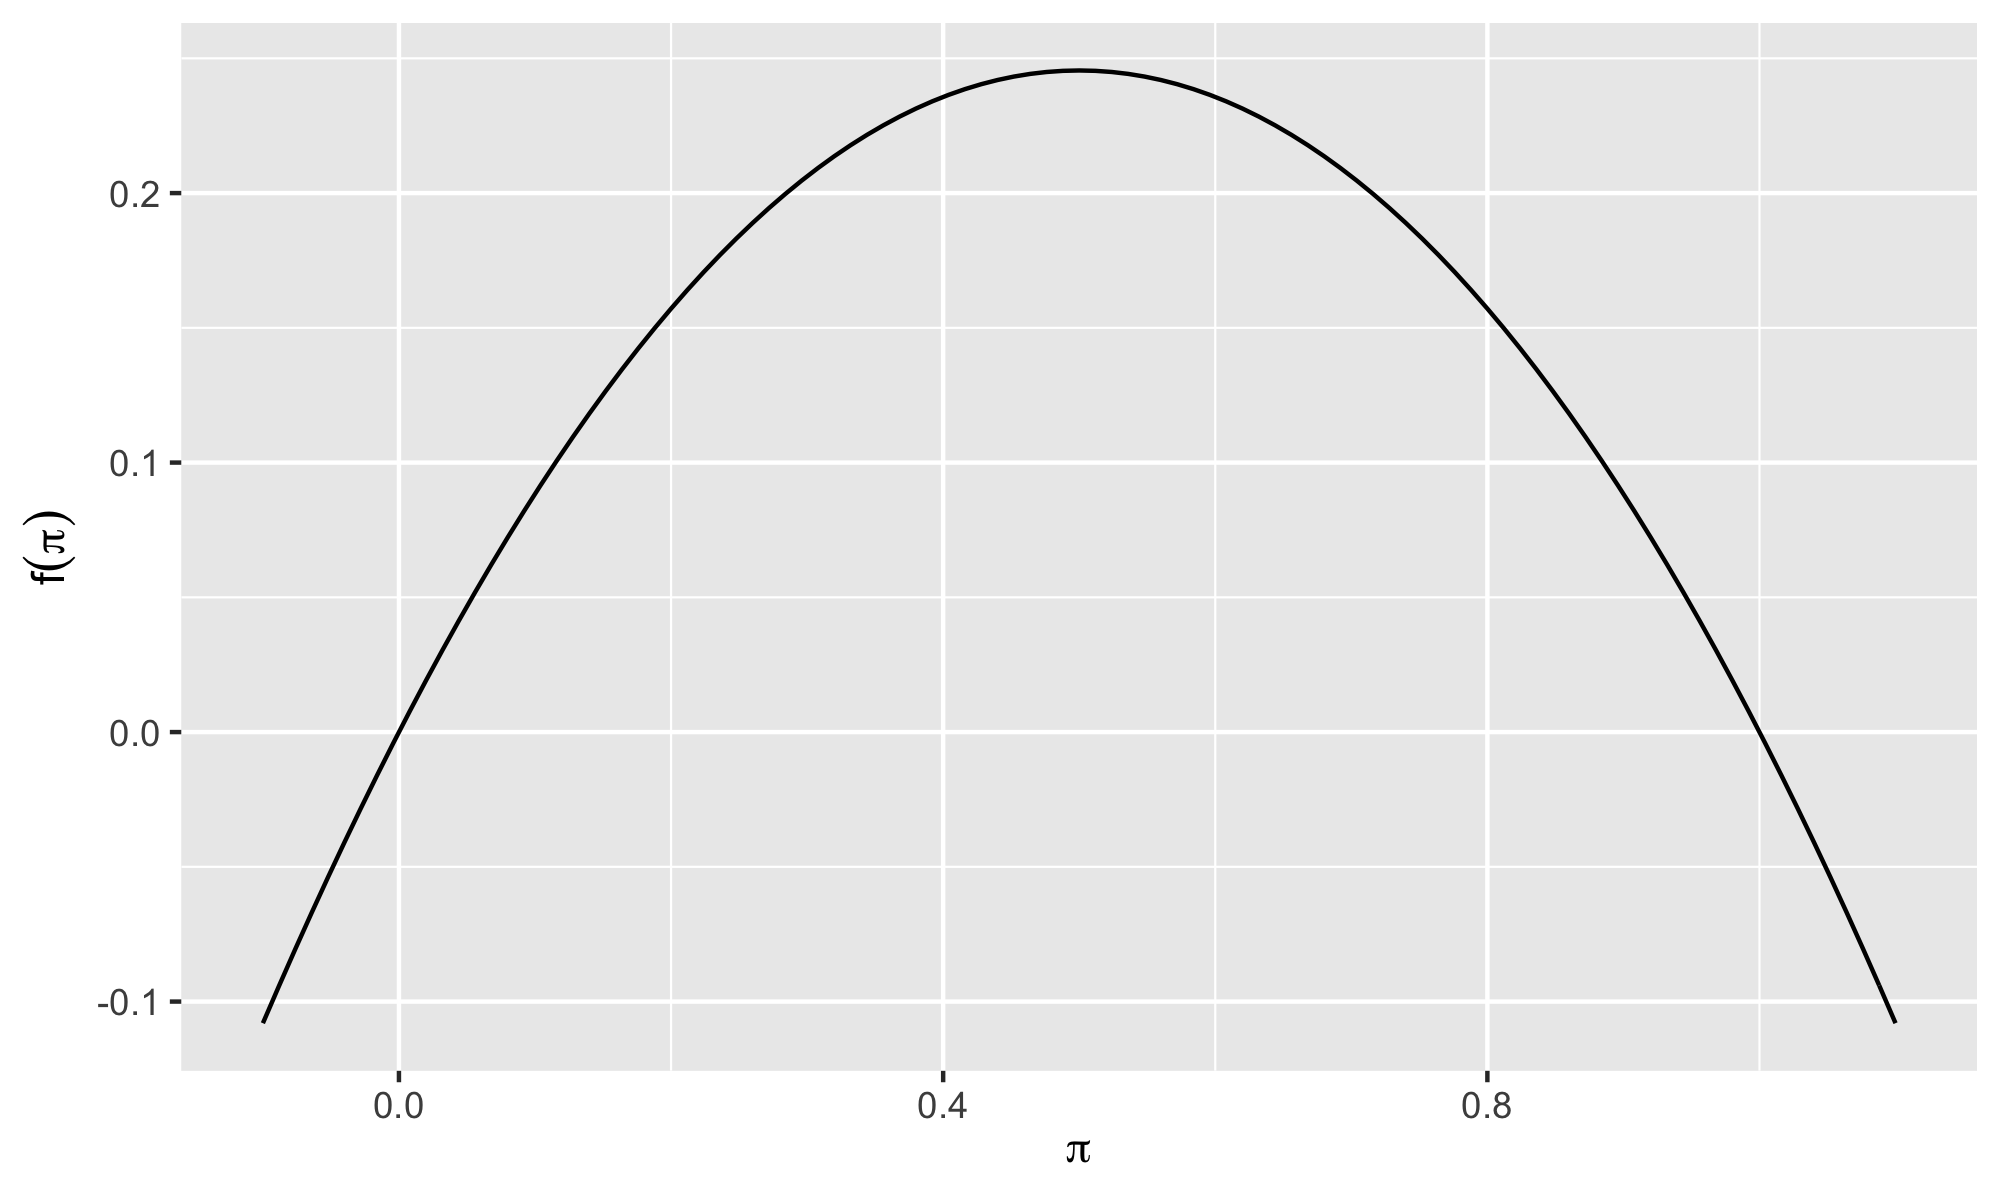
\includegraphics[width=12cm]{f-gate.png}

Similarly, \(LR(E)>1\) for any \(0< \pi <1\). Here is a plot of
\(LR(E)\) against \(\pi\):

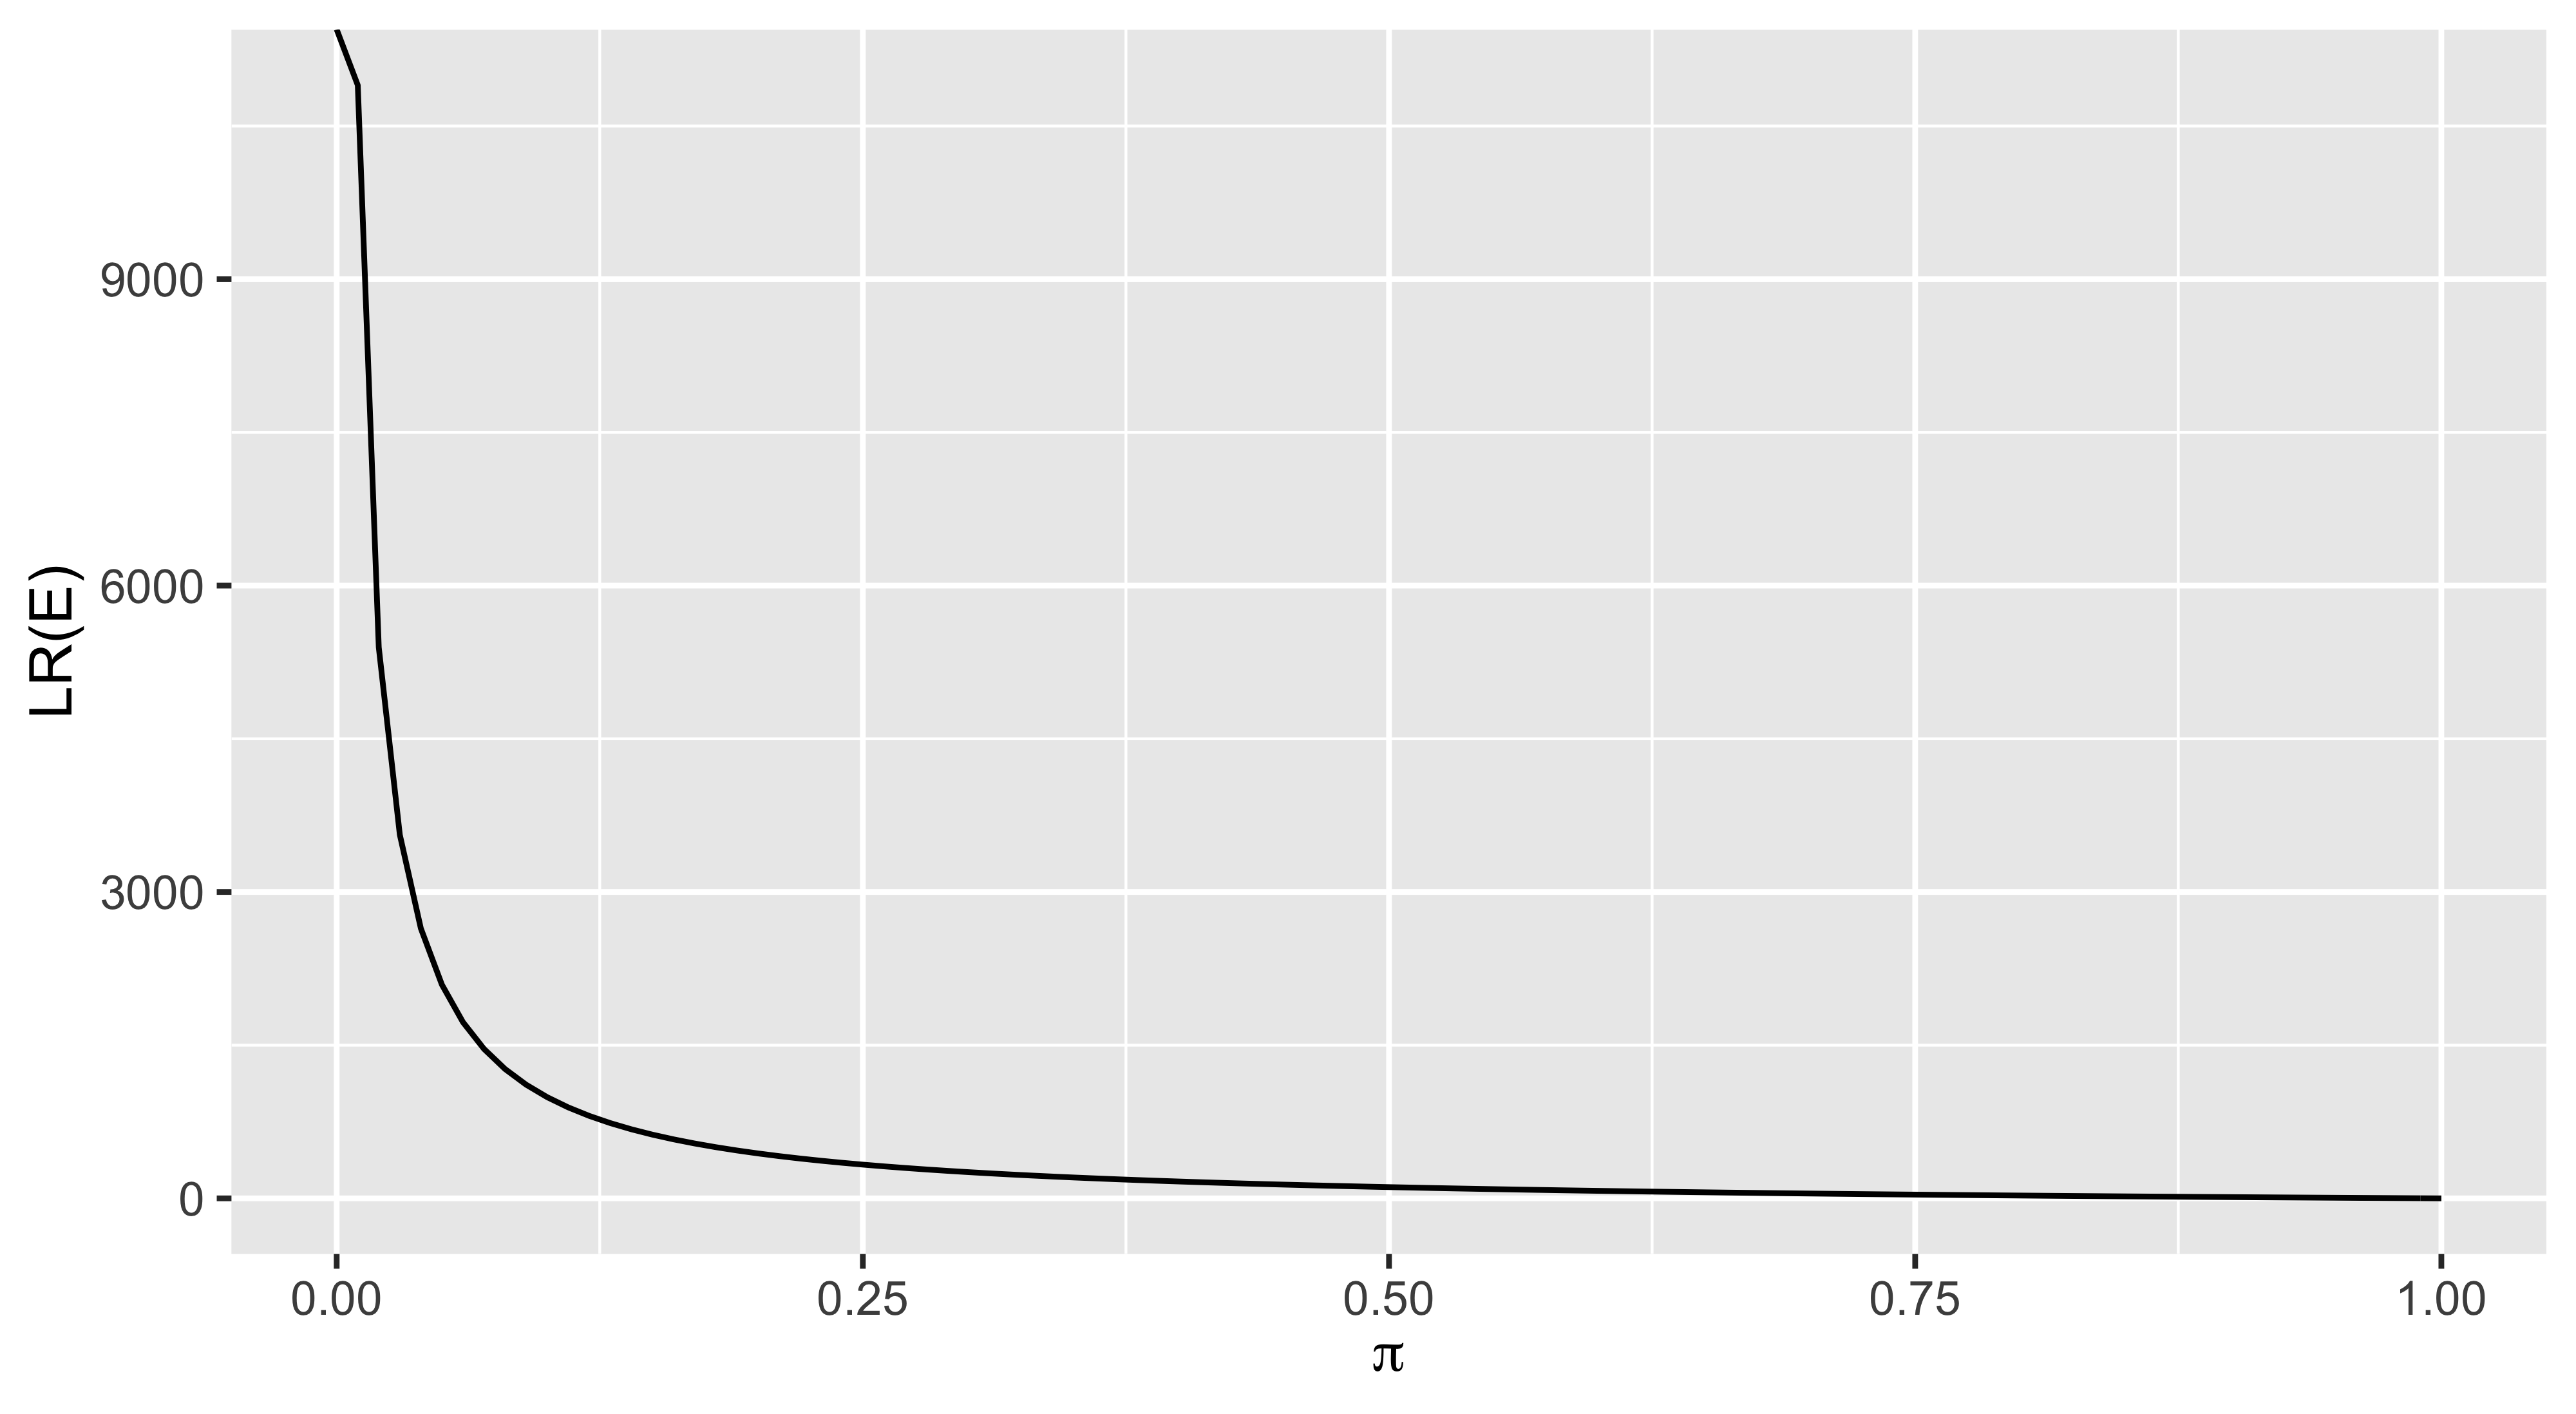
\includegraphics[width=12cm]{lre-gate.png}

\noindent Notice that \(LR(E)\) does not go below 1. This means that for
\(L=G\) in the gatecrasher scenario DTLP wold tell us to convict for any
prior probability of guilt \(\pi\neq 0,1\).

One might ask: is the conclusion very sensitive to the choice of \(L\)
and \(G\)? The answer is, not too much.

\intermezzoa

How sensitive is our analysis to the choice of \(L/G\)? Well, \(LR(E)\)
does not change at all, only the threshold moves. For instance, if
\(L/G=4\), instead of \(f\) we end up with

\begin{align*}
 f'(\pi) = - 0.955 \pi^2 + 0.955\pi &>0 
 \end{align*}

and the function still takes positive values on the interval \((0,1)\).
In fact, the decision won't change until \(L/G\) increases to
\(\approx 111\). Denote \(L/G\) as \(\rho\), and let us start with the
general decision standard, plugging in our calculations for \(LR(E)\):

\begin{align*}
LR(E) &> \frac{\pr{H_\Delta}}{\pr{H_\Pi}} \rho\\
LR(E) &> \frac{1-\pi}{\pi} \rho \\
\frac{0.991-0.991\pi}{0.009\pi} &> \frac{1-\pi}{\pi} \rho\\
\frac{0.991-0.991\pi}{0.009\pi}\frac{\pi}{1-\pi} &>  \rho\\
\frac{0.991\pi-0.991\pi^2}{0.009\pi-0.009\pi^2} &>  \rho\\
\frac{\pi(0.991-0.991\pi)}{\pi(0.009-0.009\pi)} &>  \rho\\
\frac{0.991-0.991\pi}{0.009-0.009\pi} &>  \rho\\
\frac{0.991(1-\pi)}{0.009(1-\pi)} &>  \rho\\
\frac{0.991}{0.009} &>  \rho\\
110.1111 &>  \rho\\
\end{align*}

\intermezzob

So, we conclude, in usual circumstances, DTLP does not handle the
gatecrasher paradox.

\section{Probabilistic Thresholds
Revised}\label{probabilistic-thresholds-revised}

\subsection{Likelihood ratios and naked statistical
evidence}\label{likelihood-ratios-and-naked-statistical-evidence}

\subsection{Conjunction paradox and Bayesian
networks}\label{conjunction-paradox-and-bayesian-networks}

\section{STUFF FROM SEP}\label{stuff-from-sep}

\subsection{Something to use in motivations, early in the
chapter?}\label{something-to-use-in-motivations-early-in-the-chapter}

The fallacies considered so far---base rate, prosecutor's, defense
attorney's fallacy---show how the posterior probability can be
misjudged, upwards or downwards.\\
The posterior probability of a hypothesis given the evidence \%(whose
correct assessment depends on the prior probability) should not be
confused with the strength (or probative value, weight) of the evidence
in favor of the hypothesis. To a rough approximation, the strength of an
item of evidence reflects its impact on the posterior probability given
a prior probability. Suppose the prior probability of \(H\) is extremely
low, say \(\pr(H)=0.01\%\), but taking evidence \(E\) into account
brings this probability up to 35\%, that is, \(\pr(H \vert E)=35\%\).
This is a dramatic upward shift. Even though the posterior probability
of \(H\) given \(E\) is not very high, \(E\) strongly favors \(H\).
Conversely, suppose the prior probability of \(H\) is extremely high,
say \(\pr(H)=99.9\%\), but taking evidence \(E\) into account brings
this probability down to 75\%, that is, \(\pr(H \vert E)=75\%\). This is
a dramatic downward shift. Even though the posterior probability of
\(H\) given \(E\) is still quite high, \(E\) speaks against \(H\).

\%Consider the blood stain example from \ref{sec:fallacies}. The
posterior probability given the match turned out to be an unimpressive
\(17\%\) (assuming a 1\% prior probability). But this does not mean the
match was weak incriminating evidence. After taking it into account, the
posterior probability rose from 1\% (the stipulated prior) to 17\% (the
posterior). The match strongly favored the claim that the defendant was
the source of the traces, but was not not strong enough to make it very
likely. \%Similarly, in the Collins case, the posterior probability
jumped from the \(\nicefrac{1}{6 \ million}\) prior to 70\% after taking
the match into account, still not enough for a conviction but a
remarkable increase nonetheless.

\subsection{Material on Bayes factor, LR and some
examples}\label{material-on-bayes-factor-lr-and-some-examples}

One measure of the strength of evidence is the Bayesian factor
\(\nicefrac{\pr(E \vert H)}{\pr(E)}\). \%The Bayesian factor is a
probabilistic measure of the extent to which the evidence, regardless of
the absolute posterior probability, supports or does not support the
hypothesis. This is an intuitively plausible measure of evidential
strength. Note that by Bayes' theorem \% \%

\begin{align*}\pr(H \vert E) & = \textit{BayesianFactor}(H, E) \times \pr(H),\end{align*}

\% and thus the Bayesian factor is greater than one if and only if the
posterior probability \(\pr(H \vert E)\) is higher than the prior
probability \(\pr(H)\). \%\(\pr(H)<\pr(H\vert E)\), . \%So \(E\)
\textit{positively} supports \(H\) whenever the Bayesian factor is
greater than one. The greater the Bayesian factor (for values above
one), the greater the upward shift from prior to posterior probability,
the more strongly \(E\) positively supports \(H\). \%The posterior
probability of \(H\) given \(E\) could still be low even if the Bayesian
factor is significantly above one. \%Conversely, \%again by Bayes'
theorem, \%the probability of \(H\) given \(E\) is lower than the
probability of \(H\) \%, \(\pr(H)>\pr(H\vert E)\), \%if and only if the
Bayesian factor is less than one. \%So \(E\) \textit{negatively}
supports \(H\) whenever the Bayesian factor is less than one.
Conversely, the smaller the Bayesian factor (for values below one), the
greater the downward shift from prior to posterior probability, the more
strongly \(E\) negativey supports \(H\). If \(\pr(H)=\pr(H\vert E)\) the
evidence has no impact, upwards or downwards, on the prior probability
of \(H\). \%So long as the Bayesian factor is greater than one, the
evidence supports the hypothesis. If it is negative, the evidence
negatively supports the hypothesis. If it equals one, the evidence is
irrelevant.

\%There are important differences between the likelihood \%ratio and the
Bayesian factor as measures of the strength of evidence. \%The
likelihood ratio is alike the Bayesian factor
\(\nicefrac{\pr(E \vert H)}{\pr(E)}\). They are both measures of the
extent to which the evidence favors (or does not favor) a hypothesis of
interest.

The Bayesian factor \(\nicefrac{\pr(E \vert H)}{\pr(E)}\) is an absolute
measure of \(E\)'s support toward \(H\) since it compares the
probability of \(E\) under hypothesis \(H\) against the probability of
\(E\) in general. The denominator is calculated following the law of
total probability: \%

\begin{align*}\pr(E)= \pr(E \vert H) \pr(H)+\pr(E \vert \neg H) \pr(\neg H).\end{align*}

\% The catch-all alternative hypothesis \(\neg H\) can be replaced by a
more fine-grained set of alternatives, say \(H_1, H_2, \dots H_k\),
provided \(H\) and its alternatives cover the entire space of
possibilities. The law of total probability would then read: \%

\begin{align*}
\pr(E) & = \pr(E\vert H)\pr(H) +\sum_{i=1}^k \pr(E\vert H_i)\pr(H_i). 
\end{align*}

\%, just like \(H\) and its negation.

Some might worry that assessing the strength of evidence in this way
would impose too great a cognitive burden, since it would require
sifting through the entire space of possibilities, a seemingly
impossibly task. \%This is is certainly true if \(\pr(E)\) is calculated
by applying the law of total probability. \%But the law of total
probability \%does not mandate how \(\pr(E)\) should be assessed.
Rather, it places a coherence constraint on probability assignments. But
this need not be the case. In some cases, it might be possible to assess
\(\pr(E)\) by considering a more manageable set of alternative
hypotheses, say, only those hypotheses the litigants disagree about. So
long as the hypotheses are justifiably believed to be mutually exclusive
and jointly exhaustive, the reasoning goes through. Suppose \(H\) is the
hypothesis put forward by the prosecutor and \(H_1\) and \(H_2\) are the
only alternative hypotheses that the defense deems plausible. If neither
side finds \(H_3, H_4, \dots, H_k\) worthy of consideration, the prior
probability of these hypotheses can be conveniently set to zero. The law
of total probability would then simplify to a more manageable formula:
\%

\begin{align*}
\pr(E) & = \pr(E\vert H)\pr(H) + \pr(E\vert H_1)\pr(H_1) + \pr(E\vert H_2)\pr(H_2).%
\end{align*}

\% In this way, the litigants would no longer need to sift through the
entire space of possibilities, but only through those that they deemed
worth considering.

\%, just like \(H\) and its negation. \%

\%This need to always be the case, however. \%In fact, what one is
epistemically required to do and why is not determined by the formula.
Sometimes, direct assessment of the prior is easier than reaching it by
LOTP, sometimes not. Moreover, it is never the case that to calculate
\(\pr(E)\) one needs to apply LOTP with respect to all possible lists of
exclusive and exhaustive hypotheses, and considering just one sensible
list for which the appropraite priors and conditional probabilities are
available might be not such a huge burden. Crucialy, LOTP \%and requires
that \(Pr(E)\) depends on weighted sum of \(Pr(E | H)\) for evepossible
hypotheses. This does not mean that, in each and every case, the
asessnment of \%\(\pr(E)\) by looking the entire space of all possible
hypothesis. Sometimes is may even be possible to assess \(\pr(E)\)
upfront. \%Equally well, you can start with establishing \(\pr(E)\)
first---in such a case, LOTP will constraint the interaction of your
conditional probabilities of type \(\pr(E\vert H_i)\) and \(\pr(H_i)\).

The task of assessing the strength of evidence can be simplified even
further. Instead of deploying the Bayesian factor, the strength of
evidence can be assessed by means of the likelihood ratio, a comparative
measure of whether evidence \(E\) supports a hypothesis \(H\) more than
a competing hypothesis \(H'\), in symbols,
\(\nicefrac{\pr(E \vert H)}{\pr(E \vert H')}\). \%a measure of the
probability of the evidence under two hypotheses, \(H\) and \(H'\), .
The likelihood ratio is a comparative measure of whether the evidence
\(E\) supports a hypothesis \(H\) more than a competing hypothesis
\(H'\), where the two hypotheses need not cover the entire space of
possibilities. If the evidence supports \(H\) more than \(H'\), the
ratio would be above one, and if the evidence supports \(H'\) more than
\(H\), the ratio would be below one. The greater the likelihood ratio
(for values above one), the stronger the evidence in favor of \(H\) as
contrasted with \(H'\). The smaller the likelihood ratio (for values
below one), the stronger the evidence in favor of the competing
hypothesis \(H'\) as contrasted with \(H\). The likelihood ratio is a
simpler and more workable measure than the Bayesian factor, since it
does not require one to think about the probability of the evidence in
general, namely \(\pr(E)\). This apparent simplicity, however, can often
give rise to errors in the assessment of the evidence, especially if the
two hypotheses are not chosen carefully (more on this below in
\ref{subsec:chose-h}).

\% \%The likelihood ratio is used in the odd version of \%Bayes's
theorem (see earlier in \ref{sec:odd-bayes}): \%

Experts sometimes testify by offering the likelihood ratio as a measure
of the strength of the evidence. An expert, for instance, may testify
that the blood-staining on the jacket of the defendant is ten times more
likely to be seen if the wearer of the jacket hit the victim
(prosecutor's hypothesis) rather than if he did not (defense's
hypothesis) \citep[p.\ 38]{aitken2010fundamentals}. \%A similar
probabilistic measure of the strength of the evidence is the Bayesian
factor (see discussion in\textasciitilde{}\ref{sec:fallacies}). Experts
are typically advised not to comment on the posterior odds given the
evidence. The relationship between likelihood ratio
\(\nicefrac{\pr(E \vert H)}{\pr(E \vert H')}\) and posterior odds
\(\nicefrac{\pr(H \vert E)}{\pr(H' \vert E)}\) is apparent in the odds
version of Bayes' theorem (see earlier
in\textasciitilde{}\ref{sec:odd-bayes}): \%
\[\frac{\pr(H \vert E)}{\pr(H' \vert E)}= \frac{\pr(E \vert H)}{\pr(E \vert H')}\times \frac{\pr(H)}{\pr(H')}.\]
\% If the likelihood ratio is greater (lower) than one, the posterior
odds will be greater (lower) than the prior odds of \(H\). The
likelihood ratio, then, is a measure of the upward or downward impact of
the evidence on the odds of two hypotheses \(H\) and \(H'\). \%just like
the Bayesian factor is a measure of upward or downward impact of the
evidence on the probability of a hypothesis \(H\).
\%\todo{R: removed the following bit in light of my addition about LOTP and in light of my addition about the prior}
\%The difference is that the Bayesian factor require that \(E\) be
assessed in relation to an exhaustive space of hypotheses, while \%The
likelihood ratio only requires that \(E\) be assessed relative to two
\%hypotheses which need not cover the entire space. \% As Bayes's
theorem makes clear, an assessment of the posterior odds will require a
judgment about the prior odds, and the latter lies beyond the competence
of an expert. A prominent forensic scientist recommends that experts
`not trespass on the province of the jury \%by commenting directly on
the accused's guilt or innocence, \dots and should generally confine
their testimony to presenting the likelihood of their evidence under
competing propositions' \citep[p.\ 42]{aitken2010fundamentals}.

A potential competitor of the likelihood ratio as a measure of
evidentiary strength is an even simpler notion, the probability
\(\pr(E \vert H)\). It is tempting to think that, whenever
\(\pr(E \vert H)\) is low, \(E\) should be strong evidence against
\(H\). \%and in favor of an alternative hypothesis. Consider an example
by \cite{robertson2016interpreting}. In a child abuse case, the
prosecutor offers evidence that a couple's child rocks and that only 3\%
of non-abused children rock,
\(\pr(\textsf{child rocks} \vert \textsf{no abuse})=3\%\). If it is
unlikely that a non-abused child would rock, the fact that this child
rocks might seem strong evidence of abuse. But this reading of the 3\%
figure is mistaken. It could well be that 3\% of abused children rock,
\(\pr(\textsf{child rocks} \vert \textsf{abuse})=3\%\). \%The two
probabilities, \(\pr(\textsf{child rocks} \vert \textsf{abuse})\) and
\(\pr(\textsf{child rocks} \vert \neg \textsf{abuse})\), need not add up
to 100\%, and If rocking is unlikely under either hypothesis---which
means the likelihood ratio
\(\nicefrac{\pr(\textsf{child rocks} \vert \textsf{abuse})}{\pr(\textsf{child rocks} \vert \textsf{no abuse})}\)
equals one---rocking cannot count as evidence of abuse. Thus, in order
to avoid exaggerations of the evidence, it is best to assess the
evidence by means of the likelihood ratio rather the probability of the
evidence given a hypothesis
\citep{Royall1997, triggsCommentWhyEffecta, enfs2015}.

\%This observation applies generally to all forms of evidence, inclusive
of DNA evidence, although it might not always make a practical
difference. \%For suppose an expert testifies that the crime traces
genetically \%match the defendant and that the random match probability
is extremely low, say 1 in 100 million. Is the match strong evidence
that the defendant is the source of the traces? The random match
probability---often interpreted as the probability that someone who is
not the source would coincidentally match,
\(\pr(\textsf{match} \vert \neg \textsf{source})\)---is a common measure
of the strength of a DNA match. The lower this probability, the more
strongly incriminating the match. This is sensible because a low random
match probability suggests it is unlikely two people could share the
same DNA profile. Yet, strictly speaking, a match is strong evidence
that the defendant is the source only if \%the probability that the
person who left the traces (the `source') would match is significantly
greater than the probability that a random person (someone who is not
the source) would also match, or in other words, \%Formally, if
\%\(\pr(\textrm{DNA match} \vert \neg \textsf{source})\) is low, the DNA
match is strong incriminating evidence only if
\(\pr(\textsf{DNA match} \vert \textrm{source})\) is much higher. \%only
if \%the likelihood ratio
\(\nicefrac{\pr(\textsf{DNA match} \vert \textsf{source})}{\pr(\textsf{DNA match} \vert \neg \textsf{source})}\)
is significantly greater than one. A low random match probability just
means that the denominator is low. If the numerator is equally low, the
match would be worthless evidence. \% \% This conceptual point, however,
often does not make a difference in practice. The probability that
someone who is the source would match,
\(\pr(\textsf{match} \vert \textsf{source})\), should be high so long as
the test has a low false negative rate. \%Assuming
\(\pr(\textsf{match} \vert \textsf{source})\) is high, \% That
\(\pr(\textsf{match} \vert \neg \textsf{source})\) is low should be
enough to ensure that the likelihood ratio is significantly above one.
For practical purposes, then, a suitably low random match probability
does count as strong incriminating evidence. But the conceptual point
still stands.

\subsection{Cold-hit}\label{cold-hit}

\todo{I would seriously consider having an extensive section illustrating the utility of LR with the case of cold hits, including the details that were commented out in SEP, I'm pasting this here, we'll discuss it tomorrow.}

\subsection{Cold-hit DNA matches}
 \label{subsec:cold-hit}

To better appreciate the theoretical virtues of likelihood ratios, it is
instructive to look at a case study, DNA evidence, focusing in
particular on so-called cold-hit matches. DNA evidence is one of the
most widely used forms of quantitative evidence currently available.\\
It may be used to corroborate other evidence in a case or as the primary
incriminating evidence. For example, suppose different investigative
leads point to an individual, Mark Smith, as the perpetrator. The
investigators also find several traces at the crime scene left by the
perpetrator. Laboratory analyses show that the genetic profile
associated with the traces matches Smith. In this scenario, the DNA
match corroborates the other evidence against Smith. In contrast,
suppose the police has no other investigative lead except the traces
left at the crime scene. Hoping to find the perpetrator, the police run
the genetic profile associated with the traces through a database of
profiles and find a match, a so-called \textit{cold-hit}. \%---the
individual with the matching profile can face trial and possibly a
conviction. \%When it is presented as evidence of guilt, a DNA match
will often supplement other evidence, such as evidence from police
investigation. \%Consider, for example, the California murder case of
Diana Sylvester. \% There is a rich scholarly debate about cold-hit
matches and how to correctly assess their probative value. Cold-hit DNA
matches have been the focus of intense discussion in recent years. Since
in cold-hit cases there is little or no other evidence, cold-hit matches
are often the primary item of evidence against the defendant. Some
believe that this circumstance weakens the match. Others disagree. This
debate illustrates how probability theory---in particular, the
likelihood ratio---can help to assess the strength of evidence at trial.
What follows examines some of the main arguments.

\%There is a rich scholarly debate about DNA matches and how to
correctly assess their probative value. \%This observation applies
generally to all forms of evidence, inclusive of DNA evidence, although
it might not always make a practical difference.

\paragraph{Random match v. database match}

Suppose an expert testifies that the crime traces genetically match the
defendant and that the random match probability is extremely low, say 1
in 100 million. \%Is the match strong evidence that the defendant is the
source of the traces? The random match probability---often interpreted
as the probability that someone who is not the source would
coincidentally match,
\(\pr(\textsf{match} \vert \neg \textsf{source})\)---is a common measure
of the strength of a DNA match. The lower this probability, the more
strongly incriminating the match. \%The rationale here is that a low
random match probability suggests that it is unlikely that two people
would share the same DNA profile. But, strictly speaking, a match is
strong evidence that the defendant is the source only if \%the
probability that the person who left the traces (the `source') would
match is significantly greater than the probability that a random person
(someone who is not the source) would also match, or in other words,
\%Formally, if \%\(\pr(\textrm{DNA match} \vert \neg \textsf{source})\)
is low, the DNA match is strong incriminating evidence only if
\(\pr(\textsf{DNA match} \vert \textrm{source})\) is much higher. \%only
if the likelihood ratio
\(\nicefrac{\pr(\textsf{DNA match} \vert \textsf{source})}{\pr(\textsf{DNA match} \vert \neg \textsf{source})}\)
is significantly greater than one. A low random match probability just
means that the denominator is low, and if the numerator is equally low,
the match would effectively be worthless evidence. \% This point, albeit
conceptually correct, often does not make a difference in practice.\\
\%Assuming \(\pr(\textsf{match} \vert \textsf{source})\) is high, That
the random match probability is low---that is,
\(\pr(\textsf{match} \vert \neg \textsf{source})\) is low---should be
enough to ensure that the likelihood ratio is significantly above one.
After all, the probability that the individual who is the source would
match, \(\pr(\textsf{match} \vert \textsf{source})\), should be high so
long as the test has a low false negative rate. For practical purposes,
then, a low random match probability does count as strong incriminating
evidence.

When it comes to cold-hit matches, however, further complications
emerge. \%The random match probability is no longer \%an acceptable
measure of the evidentiary value of the DNA match. To see what is at
stake, the Puckett case can serve as an illustration. In 2008, John
Puckett was identified through a database search of 338,000 profiles. He
was the only individual in the database who matched the traces collected
from Diana Sylvester, a victim of rape in 1972. The expert witness
testified that \% this particular pattern of alleles is (conservatively)
expected to Puckett's genetic profile should occur randomly among
Caucasian men with a frequency of 1 in 1.1 million. This would seem
strong evidence against Puckett. \%The ansere would be affirmativewould
be the case with an ordinary DNA match? But the DNA expert for the
defense, Bicka Barlow, pointed out that \%this was a cold-hit case.
besides the cold-hit match the evidence against Puckett was slim. It
included Puckett's previous rape convictions, a \textit{modus operandi}
common to this and previous crimes, and the fact that Puckett was in the
area. Barlow argued that the correct assessment of the cold-hit match
required to multiply 1/1.1 million by the size of the database. Call the
result of this multiplication the \textit{database match probability}.
Multiplying 1/1.1 million by 338,000 gives a database match probability
of roughly 1/3, a rather unimpressive figure. \% a less impressive
number than 1 in 1.1 million. \%\%\%If the random mat chrobability is
1/n and the database has size k, the multiplication would yield
\(1/n\times k\). \%The result of this multiplication is the \%the
Database Match Probability. \%According to this calculation, it was no
longer very unlikely that a person from the database would match. If
someone in the database could match with a probability as high as 1/3,
the cold-hit match should no longer count as strong evidence against
Puckett. At least, this was Barlow's argument.

\%Barlow's assessment of the cold-hit match is by no means
uncontroversial. Some argue it is correct and others that it is
mistaken.

\%\paragraph{NRC II recommendations and their problems}

Barlow followed a 1996 report by the National Research Council called
NRC II \%\todo{R: moved stuff to fn to avoid ambiguity.}
\citep{NRCII1996}. This report was preceded by an earlier report on DNA
evidence called NRC I \citep{NRCI1992}. NRC II recommended that in
cold-hit cases the random match probability \%(RMP) should be multiplied
by the size of the database, yielding the database match probability.
\%, precisely what Barlow did. \%(DMP). \% \%The NRC formed the
Committee on DNA Technology in Forensic Science, which issued its first
report, NRC I, in 1992 . In that report they advised against using cold
hit results as evidence, and insisted that only the frequencies related
to loci not used in the original identification should be presented at
trial. \% \%This recommendation has been criticized by many because it
underestimates the value of cold-hit matches. Presumably, \%As a
consequence, the larger the size of the data, the higher the database
match probability, the lower the strength of the match. This correction
was meant to guard against the heightened risk of mistaken matches for
the innocent people in the database. \%As seen from the debate
surrounding the Diana Sylvester case, one factor that can increase the
confusion is that when we focus on the frequency of matches found in
large databases, extremely low Random Match Probability might seem in
stark contrast with fairly high frequency of matches found. \% For
instance, the Arizona Department of Public Safety searched for matching
profiles in a database comprising 65,000 individuals. The search found
122 pairs of people whose DNA partially matched at 9 out of 13 loci; 20
pairs people who matched at 10 loci; and one pair of people who matches
at 12 loci. So it is not that unlikely to find two people in a database
who share the same genetic profiles. This argument was actually used by
John Puckett's defense attorney in the Diana Sylvester case. \% \%NRC II
offered two arguments in support of its recommendation, both of which
have been criticized by \citet{donnelly1999DNADatabaseSearches}. \%We'll
only look briefly at the key issues. \%One argument (let's call it the
\emph{frequentist} argument) had to do with Database Match Probability
(DMP). The committee compared a database trawl to multiple hypothesis
testing, which is not a good practice in light of classical statistical
methods. NRC II used an analogy. \%NRC explained the idea in terms of
coin tosses: If you toss several different coins at once and all show
heads on the first attempt, this seems strong evidence that the coins
are biased. If, however, you repeat this experiment sufficiently many
times, it is almost certain that at some point all coins will land
heads. \%you will encounter a toss in which all coins show heads. This
outcome should not count as evidence that the coins are biased.
According to NRC II, repeating the coin toss experiment multiple times
is analogous to trying to find a match by searching through a database
of profiles. As the size of the database increases, \%and the number of
attempts at finding a match also increases, it is more likely that
someone in the database who had nothing to do with the crime would
match. \% \%Let \(\gamma\) be the Random Match Probability (RMP). \% \%
\%\paragraph{Shortcomings of the database match probability}

It is unclear how the analogy with coin tossing translates to cold-hit
cases \citep{donnelly1999DNADatabaseSearches}. Searching a larger
database no doubt increases the probability of finding a match at some
point. But judges and jurors should not be concerned with \%the
probability of the statement \%The NRC II recommendation pertained to
the probability of the statement
\texttt{At\ least\ one\ of\ the\ profiles\ in\ the\ database\ \%of\ size\ \$d\$\ \ would\ randomly\ match\ the\ crime\ sample.\textquotesingle{}\ \%Call\ it\ the\ general\ match\ hypothesis.\ \ \%This\ statement\ has\ probability\ \$(d+1)\textbackslash{}times\ p\$,\ where\ \$p\$\ is\ the\ random\ match\ probability\ and\ \$d+1\$\ is\ the\ database\ size.\ \ \textbackslash{}todo\{Is\ this\ right?\ You\ have\ d+1.\ Why?\}\ \%\ \ \%are\ interested\ in\ whether\ a\ particular\ defendant\ is\ the\ source\ of\ the\ crime\ traces.\ \%They\ are\ concerned\ with\ the\ statement}The
profile of the particular defendant on trial would randomly match the
crime sample.`Call this the particular match hypothesis. \%and the
probability of at least one false positive. \%So what is of interest is
the probability of the particular, not the general match hypothesis. \%
This is in line with the general idea that one should update on total
available evidence: the claim that the defendant's profile match entails
but is not entailed by the claim that at least one of the database
profiles match, and so it is the former and not the latter that the
fact-finders should rely on. \% They should be concerned with \%the
probability of the statement `The profile of the defendant on trial
would randomly match the crime sample.' The probability of finding a
match between the defendant and the crime sample does not increase
because other people in the database are tested. In fact, suppose
everyone in the world is recorded in the database. A unique cold-hit
match would then be extremely strong evidence of guilt since everybody
would be excluded as a suspect except one matching individual. Instead,
if the random match probability is multiplied by the size of the
database, the probative value of the match in this case should be quite
low. This is counter-intuitive.\%\\
\%Even without a world database, the NRC II proposal remains problematic
since it sets up a way for defendant to arbitrarily weaken the weight of
cold-hit DNA matches. It is enough to make more tests against more
profiles in more databases. Even if all the additional profiles are
excluded (intuitively, pointing even more clearly to the defendant as
the perpetrator), the NRC II recommendation would require to devalue the
cold-hit match even further. \%
\footnote{The Database Match Probability is not a real probability either. Suppose a given profile frequency is $
\nicefrac{1}{10}$ and one searches for this profile in a database of size 10. Does the  probability of a match  equal $\nicefrac{1}{10}\times 10=1$? Surely not. Assuming the matches are independence, % of $\textrm{no match}$ for the  members of the database, it is
this probability should be
\begin{align*}
1-\pr(\textrm{no match}) & = 1- \left(\nicefrac{9}{10}\right)^{10}\\
& = 1- 0.3486784 \approx 0.65.
\end{align*}} \%Multiplication by database size would be appropriate if
the matches excluded each other and thus were not independent. Suppose I
toss a die, and the database contains \(n=\) three \emph{different}
numbers: \(1, 2\) and \(3\). Then, for each element of the database, the
probability \(p\) of each particular match is \(\nicefrac{1}{6}\), and
the probability of \emph{a} match is
\(\nicefrac{1}{6}+\nicefrac{1}{6}+\nicefrac{1}{6}=\nicefrac{1}{6}\times 3 = n\times p =\nicefrac{1}{2}\).\}

\%I could use the addition between in such a situation each match
excludes other matches. I could still use \(1-\pr(\textrm{no match})\)
to calculate the same probability, but I can't calculate
\(\pr(\textrm{no match})\) by taking it to be
\(\nicefrac{5}{6}\times \nicefrac{5}{6}\times \nicefrac{5}{6} = \nicefrac{5}{6}^3 \approx 0.58\),
because the multiplication here requires independence, which is missing
(if my die result is not a 3, it's more likely to be one of the other
numbers).\}

\%A database that contained everybody however, is \%a far-fetched
possibility. At least, the NRC II recommendation could very well apply
to more limited databases. Leaving coin tossing aside, another analogy
has been used to argue that the evidentiary value of a cold-hit match
should be weakened. The analogy is between searching for a match in a
database and multiple hypothesis testing, which is a dubious research
practice. In classical hypothesis testing, if the probability of type I
error in a single test of a hypothesis is 5\%, this probability will
increase by testing the same hypothesis multiple times. The database
match probability---the argument goes---would correct for the increased
risk of type I error. This analogy with multiple testing, however, is
misplaced. As \citet{balding2002DNDatabaseSearch} points out, multiple
testing consists in testing the \textit{same} hypothesis multiple times
against new evidence. In cold-hit cases, there is no such multiple
testing. \%there is no multiple hypothesis testing involved here.
\%Rather that the hypothesis about the suspect being formulated after
the test, Rather, multiple hypotheses---each concerning a different
individual in the database---are tested only once and then excluded if a
negative match occurs. \%before the search multiple individual
hypotheses about each of potential suspects in the database are
formulated, and each of them is tested once during the search. From this
perspective, the hypothesis that the defendant is the source was one of
the many hypotheses subject to testing. The cold-hit match supports that
hypothesis and rules out the others.

Perhaps, there is a better analogy here
\citep[p.\ 950]{donnelly1999DNADatabaseSearches}. Imagine a biased coin
whose physical appearance is indistinguishable from the fair coins in a
piggy bank. The biased coin is the perpetrator and the piggy bank is the
database containing innocent people. After the biased coin is thrown
into the bank with the other coins, someone picks out a handful of coins
at random and flips each of them twenty times. Each coin lands heads
approximately ten times---except for one coin, which lands heads on all
twenty flips. The fact that other coins seem unbiased makes the claim
that this one is biased\\
better supported since at least one coin in the bank must be biased. \%
\% Contrary to NRC II, \cite{donnelly1999DNADatabaseSearches} argue that
if potential suspects in the database are excluded as sources, this
should increase, not decrease, the probability that the defendant who
matches the crime traces is the source. A cold-hit match, then, is
stronger and not weaker evidence of guilty than ordinary DNA matches.

\paragraph{The likelihood ratio of cold-hit matches}

\%NRC II made another recommendation. They recommended that in cold-hit
cases the likelihood ratio \(R\) associated with the DNA match should be
divided by the size of the database \(d+1\). This recommendation, too,
is questionable. Suppose \(R\) is not too high, say because the
identified profile is common since the crime scene DNA is degraded and
only a few markers could be used. Then, \(d+1\) can be greater than
\(R\), so \(R/(d+1)<1\). The match would then be exculpatory, a very
counter-intuitive result. The recommendation seems mistaken on more
general grounds, as well. If the defendant on trial is the source, the
probability that he would match is practically 1. If he is not, the
probability that he would still match equals the random match
probability. Neither of these probabilities change because other
suspects have been tested in the database search. In fact, if potential
suspects are excluded as potential sources,this should increases, not
decrease, the probability that the defendant who matches the crime
traces is the source.

A more principled way to assess cold-hit matches, one based on the
likelihood ratio, exists. The proposal draws from the literature on the
so-called \emph{island problem}, studied by
\citet{eggleston1978evidence}, \citet{dawid1994island}, and
\citet{dawid1996CoherentAnalysisForensic}. Let the prosecutor's
hypothesis \(H_p\) be
\texttt{The\ suspect\ is\ the\ source\ of\ the\ crime\ traces\textquotesingle{}\ and\ the\ defense\textquotesingle{}s\ hypothesis\ \$H\_d\$\ be}The
suspect is not the source of the crime traces'. Let \(E\) be the DNA
match between the crime stain and the suspect (included in the database)
and \(D\) the information that no one among the \(N-1\) profiles in the
database matches the crime stain. The likelihood ratio associated with
\(E\) and \(D\) should be
\citep{balding1996EvaluatingDNAProfilea, taroni2006bayesian}: \%

\begin{align*}
V & = \frac{\pr(E,D\vert H_p)}{\pr(E,D\vert H_d)}.
\end{align*}

\% Since \(\pr(A\wedge B)=\pr(A\vert B)\pr(B)\), for any statement \(A\)
and \(B\), this ratio can be written as \%

\begin{align*}
V & = \frac{\pr(E\vert H_p,D)}{\pr(E\vert H_d,D)} \times \frac{\pr(D\vert H_p)}{\pr(D\vert H_d)}.
\end{align*}

\% The first ratio \(\nicefrac{\pr(E\vert H_p,D)}{\pr(E\vert H_d,D)}\)
is roughly \(\nicefrac{1}{\gamma}\), where \(\gamma\) is the random
match probability. The second ratio
\(\nicefrac{\pr(D\vert H_p)}{\pr(D\vert H_d)}\)--- call it the
\emph{database search ratio}---requires some more work. Consider first
the denominator \(\pr(D \vert H_d)\). If the suspect is not the source
(\(H_d\)), someone else is, either someone who is in the database or
someone not in the database. Let \(S\) stand for `The source is someone
in the database.' By the law of total probability, \%

\begin{align*}
\pr(D\vert H_d) & = \pr(D\vert S, H_d) \pr(S\vert H_d) + \pr(D\vert \neg S, H_d) \pr(\neg S \vert H_d). 
\end{align*}

\% If the source is someone in the database (\(S\)) and the suspect is
not the source (\(H_d\)), it is very unlikely that no one in the
database would match (\(D\)). \%the probability of \(D\) that no one
other than the suspect would match can be set to zero. So
\(\pr(D\vert S, H_d)\approx 0\). \%The above equality therefore
simplifies to \%

\begin{align*}
\pr(D\vert H_d) & =  \pr(D\vert \neg S, H_d) \pr(\neg S %\vert H_d), 
\end{align*}

The database search ratio would therefore be: \%

\begin{align*}
\frac{\pr(D\vert H_p)}{\pr(D\vert H_d)} & = \frac{\pr(D\vert H_p)}{\pr(D\vert \neg S, H_d) \pr(\neg S \vert H_d)}.
\end{align*}

\% Note that \(\pr(D\vert H_p)=\pr(D\vert \neg S, H_d)\) because whether
the suspect is the source (\(H_p\)) or not (\(H_d\)) does not affect
whether there is a match in a database that does not contain the source
(\(\neg S\)).\% \%and let ---the probability that no person in the
database other than the suspect would match (D), assuming the suspect
was in fact the source---be \(\psi_{N-1}\). \%Notice that
\(\pr(D\vert \neg S, H_d)\) \% is the probability that no one other than
the suspect matches in the database that does not contain the real
source, if the suspect is not the source. But , so this conditional
probability can also be estimated as \(\psi_{N-1}\).
\footnote{If the prior probability that the perpetrator is in the database was high, the calculations would need to be different. But normally, this prior isn't too high.}
Let \(\pr(S | H_d)=\varphi\). The database search ratio then would
reduce to \%

\begin{align*}
\frac{\pr(D\vert H_p)}{\pr(D\vert H_d)} & = \frac{1}{1-\varphi}.
\end{align*}

\% As the database gets larger, \(\varphi\) increases and the database
search ratio also increases. This ratio equals one only if no one in the
database could be the source, that is, \(\varphi=0\).

Since the likelihood ratio \(V\) of the cold-hit match results by
multiplying the likelihood ratio of the DNA match and the database
search ratio, \(V\) will always be greater than the mere likelihood
ratio of the match (except for the unrealistic case in which
\(\varphi=0\)) . Thus, a cold-hit DNA match should count as stronger
evidence than a DNA match of a previously identified suspect.
\citet{dawid1996CoherentAnalysisForensic} study different database
search strategies and consider the possibility that information about
the match is itself uncertain, but the general point remains. Under
reasonable assumptions, ignoring the database search would give a
conservative assessment of the evidentiary strength of the cold-hit
match.\footnote{\citet{donnelly1999DNADatabaseSearches}, with slightly different assumptions, derived the formula $R \times [1+mD/N]$, where $R = 1/\gamma$, $D$ is the database size, $N$ the number of people in population not in database, and $m$ is an optional multiplier reflecting how much more likely persons in the database are though to be the source when compared to the rest of the population. The expression cannot be less than $\gamma$. If no other profile has been tested, $D=0$ and LR is simply the regular DNA match LR. If $N$ is zero, that is, everyone in population is in the database, the result is infinitely large.}

This proposal is able to accommodate different competing intuitions.
First, consider the intuition that as the size of the database grows, it
is more likely that someone in the database would match. This intuition
is captured by the fact that \(\varphi\) increases proportionally to the
size of the database even though this increase does not imply that the
evidential value of the cold-hit match should decrease. Second, there is
intuitive resistance in basing a conviction on a cold-hit match,
although this resistance is less strong in case of an ordinary match
(more on this later in Section \ref{sec:naked}). This preference for
convictions based on an ordinary DNA match seems in tension with the
claim that a cold-hit match is stronger evidence of guilt than an
ordinary match. There is a way to reconcile both sides, however. The key
is to keep in mind that the evidentiary strength---measured by the
likelihood ratio---should not be confused with the posterior probability
of guilt given the evidence. \%Even if a cold-hit match is stronger
evidence of guilty, this fact does not imply that the posterior
probability of the defendant's guilt should be higher. If the cold-hit
match is the only evidence of guilt, the posterior probability of guilt
may well be lower compared to cases in which other evidence, such as
investigative leads, supplements the DNA match. This lower posterior
probability would justify the intuitive resistance towards convictions
in cold-hit cases despite the stronger probative value of cold-hit
matches in themselves.

\%Think about the following scenario: first, you identified the suspect
by some means. Then, it turned out his DNA profile matches the crime
scene stain. Fine. Now, imagine further database search for a database
not containing this suspect finds no matches. Would you think that this
information supports the guilt hypothesis? If your answer is yes, then
you do have the intuition that the lack of matches with other people
(whose profiles, in this particular case, happen to be in a database)
strengthens the evidence.

\%What about the intuition that we'd be uneasy about a conviction based
solely on a cold hit match, much less than about a DNA-match based
conviction of a previously and independently identified suspect? We
think so because now we're thinking about the posterior probability
given total evidence.

As the preceding discussion shows, the likelihood ratio is a fruitful
conceptual framework for assessing the strength of the evidence, even in
complex cases such as cold-hits. One major difficulty, however, is the
choice of the hypotheses \(H\) and \(H'\) that should be compared.
Generally speaking, the hypotheses should in some sense compete with one
another---say, in a criminal trial, \(H\) is the hypothesis put forward
by the prosecution and \(H'\) is the hypothesis put forward by the
defense. \%\todo{slightly modified the last sentence} Presumably, the
two hypotheses should be something that the two parties disagree about.
But this minimal constraint offers too little guidance and leaves open
the possibility for manipulations and misinterpretations of the
evidence. What follows outlines some of the main arguments in the
literature on this topic.

\paragraph{Ad hoc hypotheses and Barry George}

Consider a stylized DNA evidence case. Suppose the prosecutor puts
forward the hypothesis that the suspect left the traces found at the
crime scene. This hypothesis is well supported by laboratory analyses
showing that the defendant genetically matches the traces. The defense,
however, responds by putting forward the following \textit{ad hoc}
hypothesis: `The crime stain was left by some unknown person who
happened to have the same genotype as the suspect.' Since the
probability of the DNA match given either hypothesis is 1, the
likelihood ratio equals 1 \citep{evett2000MoreHierarchyPropositions}.
The problem generalizes. For any item of evidence and any given
prosecutor's hypothesis \(H\), there is an \textit{ad hoc} competing
hypothesis \(H^*\) such that
\(\nicefrac{\pr(E \vert H)}{\pr(E \vert H^*)}=1\). Hypothesis \(H^*\) is
a just-so hypothesis, one that is selected only because it explains the
evidence just as well as hypothesis \(H\) does \citep{mayo2018}. \% If
no further constraints are placed on the choice of the competing
hypotheses---it would seem---no evidence could ever incriminate a
defendant. This is unsettling. \%But this conclusion need not be so
damning in practice. Judges and jurors, however, will often recognize
\textit{ad hoc} hypotheses for what they are---artificial theories that
should not be taken seriously. Perhaps, the reasonable expectations of
the participants in a trial will suffice to constrain the choice of
hypotheses in just the right way. At the same time, real cases can be
quite complex, and it is not always obvious whether a certain choice of
competing hypotheses, which are not obviously \textit{ad hoc}, is
legitimate or not.

\%\paragraph{Barry George}

\%Even when the competing hypotheses are not obviously \textit{ad hoc},
\%the absence of a clear rationale for their choice \%may create
confusions in the assessment of the evidence.

A notable example is R.~v.~Barry George (2007 EWCA Crim 2722). Barry
George was accused of murdering TV celebrity Jill Dando. \%
\%\textbackslash{}begin\{center\}
\%\textbackslash{}begin\{tabular\}\{lp\{12cm\}\} \% \(E\) \&\\
A single particle of firearm residue \%(FDR) was found one year later in
George's coat pocket and it matched the residue from the crime scene.
This was the key incriminating evidence against him.
\%\textbackslash{}end\{tabular\} \%\textbackslash{}end\{center\} \%
\%\noindent  The defense argued that, since it was only one particle,
there must have been contamination. The experts for the prosecution,
however, testified that it was not unusual that a single particle would
be found on the person who fired the gun. George was convicted, and his
first appeal was unsuccessful. \% After the first appeal, Dr.~Evett from
the Forensic Science Service worried that the evidence had not been
properly assessed at trial. The jurors were presented with the
conditional probability \%\(\pr(\textsf{residue}\vert H_d)\) of finding
the firearm residue in George's coat given the defense hypothesis
\%\(H_d\) that George \textit{did not} fire the gun. This probability
was estimated to be quite low, indicating that the evidence spoke
against the defense's hypothesis. But the jurors were not presented with
the conditional probability \%\(\pr(\textsf{residue}\vert H_p)\) of
finding the same evidence given the prosecutor's hypothesis \%\(H_p\)
that George \textit{did} fire the gun that shot Dando. \%
\%\textbackslash{}begin\{center\} \%
\textbackslash{}begin\{tabular\}\{lp\{12cm\}\} \%\(H_d\) \& BG did not
fire the gun that shot JD.\textbackslash{} \%\(H_p\) \& BG fired the gun
that shot JD. \%\textbackslash{}end\{tabular\}
\%\textbackslash{}end\{center\} \% \noindent  An expert witness,
Mr.~Keeley, was asked to provide both conditional probabilities and
estimated them to be \(\nicefrac{1}{100}\), which indicated that the
firearm residue had no probative value. \%After new guidelines for
reporting low level FDR in 2006, the FSS re-assessed the evidence and
concluded that it was irrelevant. George appealed again in 2007, and
relying on Keely's estimates, won the appeal. \%

At first, this case seems a good illustration of how likelihood ratios
help to correctly asses the value of the evidence presented at trial.
But this reading of the case would be overly optimistic. In fact, a
close study of the trial transcript shows that Keeley's choice of
hypotheses lacked coherence and the likelihood ratio based on them was
therefore meaningless \citep{fenton2014WhenNeutralEvidence}. \% \% For
instance, Mr Keeley is reported to have said: \%
\%\textbackslash{}begin\{quote\} \% It was necessary to balance the
likelihood that the particle came from a gun fired by the appellant and
the likelihood that it came from some other source. Both were unlikely
but both were possible. \%\textbackslash{}end\{quote\} \%\noindent  \%
On one occasion, Keeley compared the hypothesis that the particle found
in George's pocket came from a gun fired by George himself, and the
alternative hypothesis that the particle came from another source. \%At
the same time, Keeley said that the prior probabilities of both
hypotheses should be low, which is mathematically impossible if they
were exhaustive and exclusive.\\
On another occasion, Keeley took the prosecutor's hypothesis to be
\texttt{The\ particle\ found\ in\ George\textquotesingle{}s\ pocket\ came\ from\ the\ gun\ that\ killed\ Dando\textquotesingle{}.\ \ But\ the\ \ conditional\ probability\ of\ the\ evidence\ given\ this\ hypothesis\ should\ not\ be\ low.\ It\ should\ actually\ be\ one.\ \ \%\textbackslash{}dots\ \%\textbackslash{}begin\{quote\}\ \%\textbackslash{}dots\ \ Mr\ Keeley\ gave\ to\ us,\ this\ was\ an\ equally\ unlikely\ event,\ whether\ it\ had\ come\ from\ the\ cartridge\ that\ killed\ Miss\ Dando,\ or\ from\ some\ innocent\ source.\ \ \%\textbackslash{}end\{quote\}\ \%\ \%\textbackslash{}noindent\ Note\ that\ here\ the\ persecution\ hypothesis\ is\ taken\ to\ be:\ \textbackslash{}emph\{the\ particle\ found\ in\ BG\textquotesingle{}s\ pocket\ came\ from\ the\ gun\ that\ killed\ JD\}.\ Now,\ \$E\$\ is\ a\ logical\ consequence\ of\ this\ hypothesis,\ and\ so\ this\ likelihood\ should\ be\ 1.\ \ \ In\ some\ other\ contexts,\ Keeley\ took\ the\ defense\ hypothesis\ to\ be}The
particle on George's pocket was inserted by contamination', but again,
the conditional probability of the evidence given this hypothesis should
be one. The most charitable reading of the trial transcript suggests
that the expert had in mind the hypotheses
\texttt{George\ was\ the\ man\ who\ shot\ Dando\textquotesingle{}\ and}The
integrity of George's coat was corrupted'. But \%these hypotheses are
neither exhaustive nor exclusive, and Keeley gave no clear criterion for
why these hypotheses should be compared in the likelihood ratio
\citep[see][for further details]{fenton2014WhenNeutralEvidence}.

\paragraph{Exclusive and exhaustive?}

The confusion in the Barry George case is attributable to the absence of
clear rules for choosing the hypotheses in the likelihood ratio. One
such rule could be: pick competing hypotheses that are exclusive (they
cannot be both true) and exhaustive (they cannot be both false). In this
way, the parties would not be able to pick \textit{ad hoc} hypotheses
and skew the assessment of the evidence in their own favor. \% \%One of
the competing hypotheses in the likelihood ratio does not have to be the
negation of the other. In some cases, they could both be false (hence,
not exhaustive), and in some they could both be true (hence, not
mutually exclusive).\\
\% Besides blocking partisan interpretations of the evidence, there are
other principled reasons to follow the exclusive-and-exhaustive rule,
specifically, the fact that when the hypotheses are not exclusive or
exhaustive, the likelihood ratio delivers counterintuitive results.
\%andconfusions in the assessment of the strength of the evidence often
arise. \% \%but it is not obvious that the hypotheses selected should
always be exclusive and exhaustive. \%Whether this rule would be a good
guiding principle, however, is not clear-cut. \%

If two competing hypotheses \%\(H_p\) and \(H_d\) are not mutually
exclusive, it is possible that \%the evidence supports them to an equal
extent \%\todo{This was wrong. Fixed.} they both make the evidence
equally likely (the likelihood ratio is one), and yet the posterior
probabilities of the hypotheses given the evidence are higher than their
prior probabilities. For instance, let \(H_p\) stand for
\texttt{The\ defendant\ is\ guilty\textquotesingle{}\ and\ \$H\_d\$\ for}The
defendant was not at the crime scene'. Both hypotheses might be true.
\%Say the prior probability of both is \(50\%\). Let \(E\) stand for
\texttt{Ten\ minutes\ before\ the\ crime\ took\ place\ the\ defendant-\/-\/-seen\ at\ a\ different\ location-\/-\/-\ was\ overheard\ on\ the\ phone\ saying\ \textbackslash{}emph\{go\ ahead\ and\ kill\ him\}.\textquotesingle{}\ \ \%\$E\$\ supports\ both\ \$H\_p\$\ and\ \$H\_d\$,\ and\ \ It\ is\ conceivable\ that\ the\ likelihood\ ratio\ should\ equal\ one\ in\ this\ context,\ yet\ the\ posterior\ probabilities\ of\ each\ hypothesis,\ given\ \$E\$,\ should\ be\ higher\ than\ the\ prior\ probability.\ So,\ intuitively,\ the\ evidence\ should\ positively\ support\ each\ hypothesis,\ contrary\ to\ what\ the\ likelihood\ ratio\ would\ suggest.\ \ \%\ Further,\ when\ the\ two\ competing\ hypotheses\ are\ not\ exhaustive,\ the\ likelihood\ ratio\ may\ once\ again\ clash\ with\ our\ intuitions.\ \ \%The\ likelihood\ ratio\ might\ then\ equal\ one\ even\ though\ the\ evidence\ lowers\ their\ posterior\ probability.\ \ For\ example,\ suppose\ Fred\ and\ Bill\ attempted\ to\ rob\ a\ man.\ The\ victim\ resisted,\ was\ struck\ on\ the\ head\ and\ died.\ Say\ \$H\_p\$\ stand\ for}Fred
struck the fatal blow' and \(H_d\) stand for
\texttt{Bill\ struck\ the\ fatal\ blow.\textquotesingle{}\ The\ hypotheses\ are\ not\ exhaustive.\ A\ missing\ hypothesis\ is}The
man did not die from the blow.' Suppose \(E\) is the information that
the victim had a heart attack six months earlier. The likelihood ratio
\(\nicefrac{\pr(E \vert H_p)}{\pr(E \vert H_d)}\) equals one since
\(\pr(E\vert H_p)=\pr(E\vert H_d)\). Yet \(E\) reduces the probability
of both \(H_p\) and \(H_d\). So, in this case, the evidence should
negatively support each hypothesis, contrary to what the likelihood
ratio suggests.

Despite these problems, however, always relying on exclusive and
exhaustive hypotheses is not without complications either. For consider
an expert who decides to formulate the defense hypothesis by negating
the prosecution hypothesis, say,
\texttt{the\ defendant\ did\ not\ hit\ the\ victim\ in\ the\ head.\textquotesingle{}\ This\ choice\ of\ defense\ hypothesis\ can\ be\ unhelpful\ in\ assessing\ the\ evidence\ because\ the\ required\ probabilities\ are\ hard\ to\ estimate.\ For\ instance,\ what\ is\ the\ probability\ that\ the\ suspect\ would\ carry\ such\ and\ such\ blood\ stain\ if\ he\ did\ not\ hit\ the\ victim\ in\ the\ head?\ This\ depends\ on\ whether\ he\ was\ present\ at\ the\ scene,\ what\ he\ was\ doing\ at\ the\ time\ and\ many\ other\ circumstances.\ \%Similarly,\ in\ a\ rape\ case,\ it\ is\ hard\ to\ estimate\ the\ probability\ of\ the\ matching\ evidence\ if\ the\ suspect\ did\ not\ have\ the\ intercourse\ with\ the\ victim.\ Instead,\ what\ is\ considered\ is\ the\ hypothesis\ that\ someone\ else,\ unrelated\ to\ the\ suspect,\ had\ intercourse\ with\ the\ victim.\ \ As\ \textbackslash{}citet\{evett2000MoreHierarchyPropositions\}\ point\ out,\ the\ choice\ of\ a\ particular\ hypothesis\ to\ be\ used\ in\ the\ evaluation\ of\ the\ strength\ of\ the\ evidence\ \ \%of,\ say,\ the\ lack\ of\ semen\ in\ a\ rape\ case,\ \ \ will\ depend\ on\ contextual\ factors.\ \%Sometimes\ it\ will\ be\ \textbackslash{}emph\{intercourse\ did\ not\ take\ place\},\ sometimes\ it\ will\ be\ \textbackslash{}emph\{the\ intercourse\ took\ place,\ but\ the\ complainant\ used\ a\ vagina\ douche\},\ or\ sometimes\ \textbackslash{}emph\{another\ sexual\ act\ took\ place\}.\ \ More\ often\ than\ not,\ the\ hypotheses\ chosen\ will\ not\ be\ mutually\ exclusive.\ \ \%\ Comparing\ exclusive\ and\ exhaustive\ hypotheses\ can\ also\ be\ unhelpful\ for\ jurors\ or\ judges\ making\ a\ decision\ at\ trial.\ \ \%is\ not\ required\ for\ the\ application\ of\ Bayes\textquotesingle{}\ Theorem,\ is\ not\ the\ usual\ practice,\ and\ could\ lead\ to\ a\ \ In\ a\ paternity\ case,\ for\ example,\ \%\ in\ which\ the\ results\ of\ DNA\ profiling\ \ are\ to\ be\ evaluated,\ \ the\ expert\ should\ not\ compare\ the\ hypotheses}The
accused is the father of the child' and its negation, but rather,
\texttt{The\ accused\ is\ the\ father\ of\ the\ child\textquotesingle{}\ and}The
father of the child is a man unrelated to the putative father'
\citep{biedermann2014UseLikelihoodRatio}. The choice of the latter pair
of competing hypotheses is preferable. Even though the relatives of the
accused are potential fathers, considering such a far-fetched
possibility would make the assessment of the evidence more difficult
than needed \%Similarly, for a given DNA mixture, strictly speaking for
any \(n\) there is a hypothesis that covers the suspect and \(n\) other
unkown sources, but for sufficiently large \(n\) these are usually
discarded as unrealistic. \% \%At the same time, if the defense
hypothesis is too specific, \textit{ad hoc} and entails the evidence, it
won't be of much use. For example, take
\texttt{The\ crime\ stain\ was\ left\ by\ some\ unknown\ person\ who\ happened\ to\ have\ the\ same\ genotype\ as\ the\ suspect.\textquotesingle{}\ \%The\ probability\ of\ a\ DNA\ match\ given\ this\ hypothesis\ would\ be\ 1.\ \ \%But\ usually\ the\ probability\ of\ the\ DNA\ match\ given\ the\ prosecution\textquotesingle{}s\ hypothesis,\ say}The
crime stain was left by the suspect,' is also 1. This would result in a
rather uninformative likelihood ratio of 1 \%For example, consider the
prosecution hypothesis The probability of a match given this hypothesis
is practically 1.\% Another feature of such specific explanations is
that it's hard to reasonably estimate their prior probability, and so
hard to use them in arguments between opposing sides.
\citep{evett2000MoreHierarchyPropositions}.

\paragraph{Variability}

Any choice of competing hypotheses lies between two extremes. For one
thing, exclusive and exhaustive hypotheses guard against arbitrary
comparisons and ensure a more objective assessment of the evidence. The
drawback is that exhaustive and exclusive hypothesis cover the entire
space of possibilities, and sifting through this space is cognitively
unfeasible. So, in this respect, comparing more circumscribed hypotheses
is preferable. The danger of doing so, however, is slipping into
arbitrariness as likelihood ratios heavily depend on the hypotheses that
are compared. The more latitude in the choice of the hypotheses, the
more variable the likelihood ratio as a measure of evidentiary value.
\%It is hard not to view this variability as a sign of arbitrariness.
\%\% R; this last sentence was too much

Here is a particularly troubling \%example phenomenon.
\%\todo{changed, because this wasn't really an example.} Competing
hypotheses can concern any factual dispute, from minute details such as
whether the cloth used to suffocate the victim was red or blue, to
ultimate questions such as whether the defendant stabbed the victim.\\
As it turns out, the likelihood ratio varies across hypotheses
formulated at different levels of granularity: offense, activity and
source level hypotheses (on this distinction, see earlier in
\ref{subsec:levels}). It is even possible that, at the source level, the
likelihood ratio favors one side, say the prosecution, but at the
offence level, the likelihood ratio favors the other side, say the
defense, even though the hypotheses at the two levels are quite similar.
Further, a likelihood ratio that equals 1 when source level hypotheses
are compared may tip in favor of one side or the other when offence
level hypotheses are compared \citep{fenton2014WhenNeutralEvidence}.
This variability makes the likelihood ratio a seemingly arbitrary---and
easily manipulable---measure of evidentiary value. This is not to say
that it is unhelpful. Expert witnesses often rely on the likelihood
ratio when they assess the probative value of many forms of evidence
\citep{enfs2015}.\\
\% The likelihood ratio can be misleading, but this risk is mitigated
when its assessment is accompanied by a careful discussion of a number
of issues, such as: which hypotheses are being compared; how they are
formulated; their level of granularity (that is, source, activity and
offense level); why the hypotheses are (or are not) exclusive and
exhaustive; why other hypotheses are ruled out as unworthy of
consideration.

\%the choice of the hypotheses to be compared, their level, their being
exclusive and exhaustive (or not), the formulation of the evidential
statement, and the reasons not to use other hypotheses in the evidence
evaluation.

\%\todo{Revised this paragraph a bit, take a look again.} \%M: Great,
nice summary. I changed a few things here and there

\subsection{Even more stuff on cold hits commented out completely at the
end of the long SEP
entry}\label{even-more-stuff-on-cold-hits-commented-out-completely-at-the-end-of-the-long-sep-entry}

\%\subsection{Cold-hit DNA matches}

\%When it is presented as evidence of guilt, a DNA match will often
supplement other evidence, such as eyewitness testimony or evidence from
police investigation. At times, however, the DNA match will be the only
evidence against the defendant. This happens when the police has no
other investigative lead except the traces left at the crime scene. The
genetic profile associated with the traces can be run through a database
of profiles. If the trawl yields a match---a cold-hit---the individual
with the matching profile could face trial and possibly a conviction. \%
\%Consider, for example, the California murder case of Diana Sylvester.
In 2008, John Puckett was identified through a database search of
338,000 profiles. He was the only individual in the database who matched
the traces collected from Diana Sylvester, a victim of rape in 1972.
\%unique match to a semen DNA profile collected from a 1972 victim.
\%According to an expert witness, \% this particular pattern of alleles
is (conservatively) expected to \%Puckett's genetic profile \%should
occur randomly among Caucasian men with a frequency of 1 in 1.1 million.
This is the Random Match Probability. Although 1 in 1.1 million should
not be confused with the probability of Puckett's innocence (see
\ref{sec:fallacies} for details), the small figure indicates it is very
unlikely that a random person unrelated to the crime would match. The
match is therefore strong evidence of Puckett's guilt. During the
pretrial hearing, however, Bicka Barlow, the DNA expert for the defense,
pointed out that \%this was a cold-hit case. \%no evidence tied Puckett
to the crime other than the cold-hit match, Puckett's previous rape
convictions and the fact that he was in the area at the time of the
murder. In order to correctly assess the probative value of the cold-hit
match, Barlow argued, the random match probability should \%be
multiplied by the size of the database. Call the result of this
multiplication the \textit{database match probability}. In Puckett's
case, the multiplication of 1/1.1 million by 338,000 resulted in \%a
database match probability of roughly 1/3. \% a less impressive number
than 1 in 1.1 million. \%\%\%If the random mat chrobability is 1/n and
the database has size k, the multiplication would yield \(1/n\times k\).
\%The result of this multiplication is the \%the Database Match
Probability. \%According to this calculation, it was no longer very
unlikely that a person from the database would match. \%If someone in
the database like Puckett could match with a probability as high as 1/3,
the cold-hit DNA match was no longer strong evidence of guilt. At least,
this was Barlow's argument. \% \%This interpretation of cold-hit matches
is by no means controversial. Many argue it is mistaken. \% \%There is a
rich scholarly debate about cold-hit matches and how to correctly assess
their probative value. This section examines this debate and how
probability theory can help address it.

\%Suppose a single crime stain has been submitted to a DNA typing, and
the DNA profile of an independently apprehended suspect has been
obtained. If the profiles match, what is the evidential value of this
match? \%which would change the odds of an innocent person being a match
in Puckett's case from 1 in 1.1 million to \(\approx \nicefrac{1}{3}\).
The example illustrates that it is rather easy to be confused about the
value of a cold hit DNA evidence. How should RMP and DMP be used, if
they are to be used at all?

\%\subsection{NRC II recommendations and their problems}

\%Barlow's testimony was in agreement with a 1996 report by the National
Research Council, often called NRC II \citep{NRCII1996}. This report
should be distinguished from an earlier one called NRC I
\citep{NRCI1992}. NRC II recommended that in cold-hit cases the random
match probability \%(RMP) \%should be multiplied by the size of the
database, yielding the database match probability. \%, precisely what
Barlow did. \%(DMP). \% \%The NRC formed the Committee on DNA Technology
in Forensic Science, which issued its first report, NRC I, in 1992 . In
that report they advised against using cold hit results as evidence, and
insisted that only the frequencies related to loci not used in the
original identification should be presented at trial. \% \%This
recommendation has been criticized by many because it underestimates the
value of cold-hit matches. Presumably, \%As a consequence, the larger
the size of the data, the higher the database match probability, the
lower the strength of the match. \% This correction is meant to guard
against the heightened risk of mistaken matches for people in the
database. As the size of the database increases, \%and the number of
attempts at finding a match also increases, \% it is more likely that
someone in the database who had nothing to do with the crime could
mistakenly match. \%As seen from the debate surrounding the Diana
Sylvester case, one factor that can increase the confusion is that when
we focus on the frequency of matches found in large databases, extremely
low Random Match Probability might seem in stark contrast with fairly
high frequency of matches found. \% For instance, the Arizona Department
of Public Safety searched for matching profiles in a database comprising
65,000 individuals. The search found 122 pairs of people whose DNA
partially matched at 9 out of 13 loci; 20 pairs people who matched at 10
loci; and one pair of people who matches at 12 loci. So it is not that
unlikely to find two people in a database who share the same genetic
profiles. This argument was actually used by John Puckett's defense
attorney in the Diana Sylvester case. \% \%NRC II offered two arguments
in support of its recommendation, both of which have been criticized by
\citet{donnelly1999DNADatabaseSearches}. \%We'll only look briefly at
the key issues. \%One argument (let's call it the \emph{frequentist}
argument) had to do with Database Match Probability (DMP). The committee
compared a database trawl to multiple hypothesis testing, which is not a
good practice in light of classical statistical methods. \%To make this
point, NRC II used an analogy. \%NRC explained the idea in terms of coin
tosses: \%If you toss several different coins at once and all show heads
on the first attempt, this seems strong evidence against the hypothesis
that the coins are fair. If, however, you repeat this experiment
sufficiently many times, it is almost certain that at some point all
coins will land heads. \%you will encounter a toss in which all coins
show heads. This outcome should not count as evidence that the coins are
biased. \% \%Let \(\gamma\) be the Random Match Probability (RMP). \% \%

\%It is unclear, however, how the analogy translates to cold-hit cases.
Searching a larger database no doubt increases the probability of
finding a match at some point. But judges and jurors should not be
concerned with \%the probability of the statement \%The NRC II
recommendation pertained to the probability of the statement
\%\texttt{At\ least\ one\ of\ the\ profiles\ in\ the\ database\ \%of\ size\ \$d\$\ would\ randomly\ match\ the\ crime\ sample.\textquotesingle{}\ \%Call\ it\ the\ general\ match\ hypothesis.\ \ \%This\ statement\ has\ probability\ \$(d+1)\textbackslash{}times\ p\$,\ where\ \$p\$\ is\ the\ random\ match\ probability\ and\ \$d+1\$\ is\ the\ database\ size.\ \ \textbackslash{}todo\{Is\ this\ right?\ You\ have\ d+1.\ Why?\}\ \%\ \ \%are\ interested\ in\ whether\ a\ particular\ defendant\ is\ the\ source\ of\ the\ crime\ traces.\ \%They\ are\ concerned\ with\ the\ statement}The
profile of the particular defendant on trial would randomly match the
crime sample.`Call this the particular match hypothesis. \%and the
probability of at least one false positive. \%So what is of interest is
the probability of the particular, not the general match hypothesis. \%
This is in line with the general idea that one should update on total
available evidence: the claim that the defendant's profile match entails
but is not entailed by the claim that at least one of the database
profiles match, and so it is the former and not the latter that the
fact-finders should rely on. \% \%Rather, they should be concerned with
\%the probability of the statement `The profile of the defendant on
trial would randomly match the crime sample.' The probability of finding
a match between the particular defendant and the crime sample does not
increase because other people in the database are tested. In fact,
suppose everyone in the world is recorded in the database. In this case,
a unique cold-hit match would be extremely strong evidence of guilt
since everybody is excluded as a suspect except one matching individual.
But if the random match probability is multiplied by the size of the
database, the probative value of the match should be quite low. This is
counter-intuitive.\\
\%Even without a world database, the NRC II proposal remains problematic
since it sets up a way for defendant to arbitrarily weaken the weight of
cold-hit DNA matches. It is enough to make more tests against more
profiles in more databases. Even if all the additional profiles are
excluded (intuitively, pointing even more clearly to the defendant as
the perpetrator), the NRC II recommendation would require to devalue the
cold-hit match even further. \%

\%NRC II was concerned with the fact that in cold-hit cases the
identification of a particular defendant occurs after testing several
individuals. This concern has to do with the data-dependency of one's
hypothesis. But, as \citet{balding2002DNDatabaseSearch} points out, the
problem of data-dependency arises when the same hypothesis is tested
multiple times against new evidence. In cold-hit cases, however, there
is no multiple testing. \%there is no multiple hypothesis testing
involved here. \%Rather that the hypothesis about the suspect being
formulated after the test, \%Rather, multiple hypotheses---each
concerning a different individual in the database---are tested only once
and are excluded by a negative match. \%before the search multiple
individual hypotheses about each of potential suspects in the database
are formulated, and each of them is tested once during the search.
\%From this perspective, the hypothesis that the defendant is the source
was one of the many hypotheses subject to testing. The cold-hit match
supports that hypothesis and rules out the others.

\%Perhaps, there is a better analogy here
\%\citep[p.\ 950]{donnelly1999DNADatabaseSearches}. Imagine a coin that
is known to be biased but whose physical appearance makes it
indistinguishable from the fair coins in a piggy bank. The biased coin
is the perpetrator and the \%piggy bank is the database containing
innocent people. \%After the biased coin is thrown into the bank with
the other coins, someone picks out a handful of coins at random and
flips each of them twenty times. Each coin lands heads approximately ten
times---except for one coin, which lands heads on all twenty flips. The
fact that other coins seem unbiased makes the claim that this one is
biased better supported since at least one coin in the bank must be
biased.\% \%\textbackslash{}footnote\{Notice that the Database Match
Probability is not really a probability. Just to take a simple example,
suppose a given profile frequency is \$ \%\nicefrac{1}{10}\$ and you
search for this particular profile in a database of size 10. Does the
probability of a match equal \(\nicefrac{1}{10}\times 10=1\)? No.
Assuming the independence of \(\textrm{no match}\) for the members of
the database, it is

\begin{align*}
1-\pr(\textrm{no match}) & = 1- \left(\nicefrac{9}{10}\right)^{10}\\
& = 1- 0.3486784 \approx 0.65
\end{align*}

\%Multiplication by database size would make sense if we thought of it
as addition of individual match probabilities,
\emph{provided matches exclude each other} (and so, are not
independent). Suppose I toss a die, and my database contains \(n=\)
three \emph{different} numbers: \(1, 2\) and \(3\). Then, for each
element of the database, the probability \(p\) of each particular match
is \(\nicefrac{1}{6}\), and the probability of \emph{a} match is
\(\nicefrac{1}{6}+\nicefrac{1}{6}+\nicefrac{1}{6}=\nicefrac{1}{6}\times 3 = n\times p =\nicefrac{1}{2}\).
I could use the addition between in such a situation each match excludes
other matches. I could still use \(1-\pr(\textrm{no match})\) to
calculate the same probability, but I can't calculate
\(\pr(\textrm{no match})\) by taking it to be
\(\nicefrac{5}{6}\times \nicefrac{5}{6}\times \nicefrac{5}{6} = \nicefrac{5}{6}^3 \approx 0.58\),
because the multiplication here requires independence, which is missing
(if my die result is not a 3, it's more likely to be one of the other
numbers).\} \% \%Contrary to NRC II,
\cite{donnelly1999DNADatabaseSearches} argue that if potential suspects
in the database are excluded as sources, this should increase, not
decrease, the probability that the defendant who matches the crime
traces is the source. A cold-hit match, then, is stronger and not weaker
evidence of guilty than ordinary DNA matches.

\% \%This can be made clear by relying on the likelihood ratio as a
measure of the evidential strength of the cold-hit DNA match. If the
defendant on trial is the source, the probability that he would match is
practically 1. If he is not, the probability that he would still match
equals the random match probability. Neither of these probabilities
change because other suspects have been tested in the database search.
In fact, if potential suspects are excluded as potential sources, \%this
should increases, not decrease, the probability that the defendant who
matches the crime traces is the
source.\footnote{Of course, a classical statistician might refuse to rely on Bayesian reasoning, and rely on classical hypothesis testing instead. There are various good reasons not to do so, but we'll just point out that in such a case they simply have nothing to say about the posterior probability of the identity claim.}
\% \%Since the focus should not be on the particular, not the general
match hypothesis, the coin tossing analogy does not work. \%In a DNA
trawl you're not repeating an experiment to reject a general hypothesis.
Rather, you consider a particular hypothesis
(\emph{the defendant is the source of the material}) and test once for
\emph{the defendant's profile matches the crime sample}, and once for
each claim of type
\emph{person $i$ in the database does not have a matching profile}.

\%moved this bit to a footnote

\%NRC II made another recommendation. They recommended that in cold-hit
cases the likelihood ratio \(R\) associated with the DNA match should be
divided by \(d+1\). Their first recommendation was about a correction of
the random match probability (that is, to multiply it by the size of the
database), and this second recommendation is about the likelihood ratio
(that is, to divide it by \(d+1\)). This has counterintuitive
consequences. Suppose \(R\) is not too high, say because the identified
profile is common since the crime scene DNA is degraded and only a few
markers could be used. Then, \(d+1\) can be greater than \(R\), so
\(R/(d+1)<1\). The match would be exculpatory, a very counter-intuitive
result.

\%Moreover, NRC II would entail that if the police pick a random person
from the database, test their profile and it is a match (call this
\emph{lucky strike} )and don't test other members of the database, this
evidence --- if we follow NRC II --- should be stronger than a unique
hit in a systematic database trawl, which also does not seem too
convincing. \% \%Interestingly, the frequentist argument focused on a
different hypothesis than the likelihood one. The former assessed the
probability that at least one profile in the database would match the
crime sample by chance, the latter focused on the hypothesis that
exactly one profile would match. \%In the case of frequency,
multiplication by \(D+1\) results in a conservative and imprecise
estimate, while in the case of likelihood, division by \(D+1\) is
supposed to give a precise calculation of the likelihood of a cold hit.
\%

\% \%emphasized that, in cold-hit cases, the likelihood ratio should
taken into account that the suspect is identified only after the search
not before. If this fact is not taken into account the likelihood ratio
would be data dependent. \% \%who argued that the hypotheses proposed by
the critics of NRC II are data dependent, because the suspect is
identified only after the search (see Subsection \ref{subse:LRlogical}
for further details). \%

\%Commented this out, perhaps, this is not needed

\%(3 CT 669, 675; 5 CT 1093.)11

\% How do we square the supposedly extremely low DNA profile frequency
with the seemingly high match frequency in empirical studies on existing
databases? The key difference is between the probability of a particular
previously selected profile matching one in the database, and the
probability of the database containing \emph{some} match. \%
{[}MARCELLO'S COMMENTS: YES, YOU MADE THIS POINT EARLIER WHEN YOU
CRITICIZED THE USE OF DMP, SO I DON'T THINK THIS SHOULD BE REPEATED
HERE. MAYBE YOU CAN JUST CLARIFY WHAT YOU SAID EARLIER WHEN YOU
DISTINGUISHED DMP FROM RMP?{]}

\% Continuing with the die example, say I pick number one as my
\texttt{suspect,\textquotesingle{}\textquotesingle{}\ and\ my\ database\ has\ \$n=5\$\ with\ individual}profile
frequency in the population'' of \(\nicefrac{1}{6}\). On the assumption
that the database is randomly drawn from the population (with
replacement), the probability of one of the numbers in the database
being 1 is \(\approx 1-0.6=0.4\) (notice this time the database can
contain repetitions and the sampling was random and so we can't use
addition to calculate \(\pr(\textrm{no match with 1})\)). \%
{[}MARCELLO'S COMMENT: I REALLY LOST YOU HERE. NOW YOU SEEM TO BE
ADDRESSING A DIFFERENT PROBLEM THAN COLD-HIT MATCHES. {]}

\% In contrast, there are \(6^5\) possible states of the database, and
\(6\times 5 \times 4\times 3 \times 2\) of them contain no repetitions,
so \(\pr(\textrm{no match})\) is \(\approx 0.093\) and the probability
of \emph{a} matching pair being present in the database is
\(\approx 0.91\). Intuitively, the difference arises because now we're
searching through \({ 5 \choose 2}=10\) different pairs looking for any
of the 6 possible profile matches, instead of searching through 5
profiles looking exactly for one
profile.\footnote{This is  a reformulation of the well-known birthday problem, it's just we discussed it using smaller numbers to make the considerations more intuitively compelling.}
\% {[}MARCELLO'S COMMENTS: OK, SO HERE YOU SEEM TO BE ADDRESSING ANOTHER
PROBLEM, SUCH AS BIRTHDAY PROBLEM AND RELATED. I WONDER IF THIS IS
ANOTHER PROBLEM, NOT IMMEDIATELY HAVING TO DO WITH COLD-HIT DNA MATCHES.
CAN THIS GO INTO A SEPARATE SUBSECTION? THAT MIGHT HELP ORIENT THE
READER AND NOT MAKE THIS ONE SUBSECTION SO LONG.{]}

\%\subsection{Sensitivity of LR to hypothesis choice and NRC II} \label{subsec:LRandDNA}

\%This approach has also been defended defended by
\%\citet{stockmarr1999LikelihoodRatiosEvaluating} who points out that
since the suspect is identified after the databases search, the
hypothesis is formulated \textit{ad hoc}. Without the correction, then,
the likelihood ratio would be data-dependent.

\%Recalling the discussion of sensitivity of the likelihood ratio to the
choice of hypotheses, let's take a look at an interesting attempt to
defend NRC II by \citet{stockmarr1999LikelihoodRatiosEvaluating}. He
insists that hypotheses such as
\emph{JS was one of the crime scene donors} are evidence-dependent in
the case of database search, ``since we had no way of knowing prior to
the search that Smith would be the person that matched'' (p.~672).
Instead, Stockmarr insists, we should evaluate LR using hypotheses that
can be formulated prior to the search, such as
\emph{the true perpetrator is among the suspects identified from the database}.
And indeed, the likelihood of this hypothesis is as NRC II suggests,
\(\nicefrac{k}{np}\), where \(k\) is the number of matching profiles,
\(n\) the database size, and \(p\) the random match probability
\citep[see][for a derivation]{stockmarr1999LikelihoodRatiosEvaluating}.

\%Dawid, in a discussion with Stockmarr
\citep{dawid2001CommentStockmarrLikelihood} points out that Stockmarr's
hypotheses, while not depending on the result of the search, depend on
the data themselves (because they change with the database size). More
importantly, he also indicates that Stockmarr's hypotheses are composite
and the assessment of LR therefore requires additional assumptions about
the priors. Once these are used with Stocmarr's own LR, the posterior is
the same as the one obtained using the methods proposed by the critics
of NCR II. The phenomenon is a particular case of the one we already
discussed, because Stockmarr's hypothesis and the one originally used in
the database search problem are equivalent conditional on the evidence.
This turns out to be another example of how LR on its own might be
insufficiently informative, especially when it is unclear what the
involved hypotheses
are.\footnote{See however, Stockmarr's own reply (\emph{ibidem}).}

\%\subsection{Resolving the Database Search Problem}

\%So we know not to use DMP. But the question remains: what's the
relation between the value of a DNA match in a cold hit case as compared
to a DNA match for a previously and independently identified suspect?
After all we need to have a justified stance on cold hit evidence, and
there seems to be no hope of reaching one without the tools provided by
legal probabilism.

\%Various versions of probabilistic calculations have been developed,
depending on what idealizations and additional complexities are being
considered. \%In order to better understand how to properly assess a
cold-hit match, it is instructive to consider a simple scenario, the
\emph{island problem}, studied by \citet{eggleston1978evidence},
\citet{dawid1994island}, and
\citet{dawid1996CoherentAnalysisForensic}.\todo{M: Nowhere do you talk about the island problem. Did you delete something here?}

\%\%Let \(H_p\) stand for
\texttt{The\ suspect\ is\ the\ source\ of\ the\ crime\ traces\textquotesingle{}\ and\ \$H\_d\$\ for}The
suspect is not the source of the crime traces'. Let evidence \(E\) be
the DNA match between the crime stain and the suspect (included in the
database) and \(D\) the information that no one among the \(N-1\)
profiles in the database matches the crime stain. The likelihood ratio
associated with \(E\) and \(D\) should be
\citep{balding1996EvaluatingDNAProfilea, taroni2006bayesian}: \%

\begin{align*}
V & = \frac{\pr(E,D\vert H_p)}{\pr(E,D\vert H_d)}
\end{align*}

\% \%Since \(\pr(A\wedge B)=\pr(A\vert B)\pr(B)\), for any statement
\(A\) and \(B\), this ratio can be written as \%

\begin{align*}
V & = \frac{\pr(E,\vert H_p,D)}{\pr(E\vert H_d,D)} \times \frac{\pr(D\vert H_p)}{\pr(D\vert H_d)}
\end{align*}

\% \%The ratio \(\nicefrac{\pr(E,\vert H_p,D)}{\pr(E\vert H_d,D)}\) is
roughly \(\nicefrac{1}{\gamma}\), where \(\gamma\) is the random match
probability. The ratio \(\nicefrac{\pr(D\vert H_p)}{\pr(D\vert H_d)}\)
is called the \emph{database search ratio}. To determine this ratio,
consider first the denominator \(\pr(D \vert H_d)\). If the suspect is
not the source, someone else is, either someone who is in the database
or someone not in the database. Let \(S\) stand for `The source is
someone in the database.' By the law of total probability, \%

\begin{align*}
\pr(D\vert H_d) & = \pr(D\vert S, H_d) \pr(S\vert H_d) + \pr(D\vert \neg S, %H_d) \pr(\neg S \vert H_d)  
\end{align*}

\% \%Note that if the source is someone in the database (\(S\)) and the
suspect is not the source (\(H_d\)), it is nearly impossible that no one
in the database would match (\(D\)). \%the probability of \(D\) that no
one other than the suspect would match can be set to zero.
\%\todo{Is this right? I elaborated what you had. Please check!} So
\(\pr(D\vert S, H_d)\approx 0\). The above equation \%therefore
simplifies to: \%

\begin{align*}
\pr(D\vert H_d) & =  \pr(D\vert \neg S, H_d) \pr(\neg S \vert H_d)  
\end{align*}

\% \%Let \(\pr(D\vert H_p)\) \%be \(\psi_{N-1}\). \%Notice that
\(\pr(D\vert \neg S, H_d)\) \%is the probability of a random match in a
database of size \(N-1\) not containing the the real source, and can
also be estimated as \(\psi_{N-1}\).
\todo{I don't follow the reasoning. Can you clarify? Why do these two probabilities equal the same thing?}
If \(\pr(S)=\varphi\), then the second ratio in our calculation of \(V\)
therefore reduces to: \%

\begin{align*}
\frac{\psi_{N-1}}{\psi_{N-1}(1-\varphi)} & = \frac{1}{1-\varphi}
\end{align*}

\% \%As the database gets larger, \(\varphi\) increases and the database
search ratio also increases. This ratio equals one only if no one in the
database could be the source, that is, \(\varphi=0\).

\%Since in order to obtain the likelihood ratio \(V\), the likelihood
ratio of the DNA match is multiplied by the database search ratio, the
result will alwaysbe greater than the mere likelihood ratio of the match
(except for the unrealistic case in which \(\varphi=0\)) . Thus, a
cold-hit DNA match should count as stronger evidence than a DNA match of
a previously identified suspect.
\citet{dawid1996CoherentAnalysisForensic} study variations of the
database search problem, with different search strategies and including
the possibility that information about the match is itself uncertain,
but the general point remains. Under reasonable assumptions, ignoring
the search errs on the side of
caution.\footnote{\citet{donnelly1999DNADatabaseSearches}, with slightly different assumptions, derived the formula $R \times [1+mD/N]$, where $R = 1/\gamma$, $D$ is the database size, $N$ the number of people in population not in database, and $m$ is an optional multiplier reflecting how much more likely persons in the database are though to be the source when compared to the rest of the population. The expression cannot be less than $\gamma$. If no other profile has been tested, $D=0$ and LR is simply the regular DNA match LR. If $N$ is zero, that is, everyone in population is in the database, the result is infinitely large. }

\%Think about the following scenario: first, you identified the suspect
by some means. Then, it turned out his DNA profile matches the crime
scene stain. Fine. Now, imagine further database search for a database
not containing this suspect finds no matches. Would you think that this
information supports the guilt hypothesis? If your answer is yes, then
you do have the intuition that the lack of matches with other people
(whose profiles, in this particular case, happen to be in a database)
strengthens the evidence.

\%The fact that, compared to an ordinary DNA match, a cold-hit DNA match
is stronger evidence of guilty does not imply that the posterior
probability of the defendant's guilt should be higher in cold-hit cases.
The other evidence used to first identify the suspect, jointly with the
DNA match, might result in a higher posterior probability of guilt, even
if the likelihood ratio of the cold-hit match is higher. This different
in the posterior probability of guilt accounts for the intuition that in
cold-hit cases we should resist conviction so long as the evidence only
consists of a DNA match. The resistance toward conviction should be less
strong in other cases so long as the DNA match is supplemented by other
incriminating evidence.

\%What about the intuition that we'd be uneasy about a conviction based
solely on a cold hit match, much less than about a DNA-match based
conviction of a previously and independently identified suspect? We
think so because now we're thinking about the posterior probability
given total evidence.

\subsection{Levels of Hypotheses}\label{levels-of-hypotheses}

\todo{Consider using the stuff that was  commented out! I left percentage signs.}

Difficulties in assessing probabilities go hand in hand with the choice
of the hypotheses of interest. To some approximation, hypotheses can be
divided into three levels: offence, activity, and source level
hypotheses. At the offence level, the issue is one of guilt or
innocence, as in the statement
\texttt{Smith\ intentionally\ attacked\ the\ victim\ with\ a\ knife\textquotesingle{}.\ \ At\ the\ activity\ level,\ hypotheses\ \ do\ not\ include\ information\ about\ intent\ but\ simply\ describe\ what\ happened\ and\ what\ those\ involved\ did\ or\ did\ not\ do.\ An\ example\ of\ activity\ level\ hypothesis\ is}Smith
bled at the scene.`Finally, source level hypotheses describe the source
of the traces, such as `Smith left the stains at the crime scene,'
without specifying how the traces got there. Overlooking differences in
hypothesis level can lead to serious confusions.

To illustrate, consider a case in which a DNA match is the primary
incriminating evidence. In testifying about the DNA match at trial,
experts will often assess the probability that a random person,
unrelated to the crime, would coincidentally match the crime stain
profile \%For a survey of developments and complications of this model,
see \citep{foreman2003interpreting}. The random match probability is
often an impressively low number, say 1 in 100 million or lower, at
least excluding the possibility that relatives or identical twins would
coincidentally match
\citep{donnelly1995NonindependenceMatchesDifferent}.

\%This low probability indicates that it is extremely unlikely that a
random person would match.

\%The match should count as strong evidence against the defendant \% See
\%This presentation is similar to classical hypothesis testing. In such
a context one starts by setting up a chance hypothesis, often called the
null \(H_0\), and then calculates the probability of the evidence (or
data obtained) being such as it is or more extreme on the assumption
that \(H_0\) holds. If this probability is small (conventionally, below
\(0.01\) or \(0.05\)), this counts as evidence against \%\(H_0\). But
note that just because \(\pr(E\vert H_0)\) is small, it does not follow
that, for any alternative hypothesis, \(H_*\) \(\pr(E\vert H_*)\) is
large. The latter probability could be equally low.\\
\% \%A DNA profile consists of pairs of alleles at several loci.
Individual allele probabilities are used to calculate the expected
frequency of a given profile \(\Gamma\) in a relevant population, so
that we obtain the genotype probability \(\gamma\). Assuming the
so-called Hardy-Weinberg equilibrium, \(\gamma\) can be obtained by
multiplying the allele probabilities. Very roughly, the probability of a
match at any particular locus is around \(\nicefrac{1}{10}\), and so the
probability of a match on all 20 loci used by the FBI CODIS system
should be \(\left(\nicefrac{1}{10}\right)^{20}\). \% \%Such
calculations, however, are a bit simplistic. One factor is that given
the crime stain, we already know that at least one population member has
profile \(\Gamma\), and the observation of a gene increases the chance
of another of the same type. Actual calculations are quite complicated,
\citep[see][]{taroni2006bayesian}, as we'll discuss in the section on
BNs for DNA evidence evaluation. \% \%In legal context, \(\gamma\) ---
the so-called Random Match Probability (RMP), that is, the probability
that a random person from the population matches the crime stain profile
--- is taken to be the probability that the suspect is a match if in
fact he is innocent and is usually estimated as the frequency of a given
profile in the relevant population. \% \% is not the probability of
innocence (see \ref{sec:fallacies} for details), it \% \%And yet, in
what way the match counts as evidence against the \%defendant is not
straightforward. \%Here it is paramount to avoid a number of confusions.
\% \% \%First, the random match probability is not the posterior
probability of innocence since
\(\pr(\textsf{match} \vert \textsf{innocence})\) should not be confused
with \(\pr(\textsf{innocence} \vert \textsf{match})\). \%The random
match probability speaks to the former, not the latter probability. \%To
confuse the two would be to commit the prosecutor's fallacy (see
\ref{sec:fallacies} for details). \%Second, \%Since the random match
probability low probability indicates that it is extremely unlikely that
a random person would match. It is tempting to equate the random match
probability to \(\pr(\textsf{match} \vert \textsf{innocence})\) and
together with the prior \(\pr(\textsf{innocence})\) use Bayes' theorem
to calculate\\
the posterior probability of innocence
\(\pr(\textsf{innocence} \vert \textsf{match})\). But this would be a
mistake. \% Applying Bayes' theorem is of course recommended and helps
to avoid the prosecutor's fallacy, the conflation of
\(\pr(\textsf{innocence} \vert \textsf{match})\) and
\(\pr(\textsf{match} \vert \textsf{innocence})\). \%(see
\ref{sec:fallacies} for details). The problem lies elsewhere. Equating
the random match probability with
\(\pr(\textsf{match} \vert \textsf{innocence})\) overlooks the
difference between offense, activity and source level hypothesis. It is
hasty to assume that, in one way or another, a DNA match can speak
directly to the question of guilt or innocence. Even if the suspect
actually left the genetic material at the scene---source level
proposition---the match does not establish guilt. \%The match could be
the result of a laboratory error. Or Even if the defendant did visit the
scene and came into contact with the victim, it does not follow that he
committed the crime he was accused of. \%So even if the random match
probability is usually very low, it does not follow that the posterior
probability of innocence is near the random match probability given by
the expert. \%It is true, however, that in many circumstances the random
match probability and the posterior probability of innocence given a
match would both be very low.

Few forms of evidence can speak directly to offense level hypotheses.
Circumstantial evidence that is more amenable to a probabilistic
quantification, such as DNA matches and other trace evidence, does not.
Eyewitness testimony may speak more directly to offense level
hypotheses, but it is also less easily amenable to a probabilistic
quantification. This makes it difficult to assign probabilities to
offense level hypotheses. Experts are usually not supposed to comment
directly on offense level hypotheses, but they often comment on activity
level and source level hypotheses. In moving from source to activity
level, however, additional sources of uncertainty come into play.
\%\citep{Cook1998hierarchy}. \% The assessment of activity level
hypotheses depends on additional variables other than those on which the
assessment of source level hypotheses depends. \%For example, is this
the kind of staining that would occur if the suspect kicked the victim
in the head? For example, the probability of finding such and such
quantity of matching glass if the suspect smashed the window depends on
how the window was smashed, when it was smashed, and what the suspect
did after the action. Another problem arises due to recent improvements
in DNA profiling technology \citep{Cook1998hierarchy}. Since today
investigators are able to obtain profiles from minimal amounts of
genetic material, transfer probabilities become more difficult to assess
as more opportunities of transfer arise. If small traces such as dust
speckles can be used as evidence, the possibility that the traces were
brought to the scene accidentally becomes more likely. For this reason,
moving beyond source level hypotheses requires a close collaboration
between scientists, investigators and attorneys
\citep[see][for a discussion]{Cook1998hierarchy}. \%The hypotheses
themselves are up for revision as evidence is obtained or facts about
what happened are accepted \citep{evett2000MoreHierarchyPropositions}.

\% \% \% \%Since the likelihood ratio might change with the choice of
the hypotheses, the clarity on the choice of the hypotheses, and their
level in particular, is crucial. For instance, \% \% \%

\subsection{The two-stain problem}\label{the-two-stain-problem}

\todo{Also, worth a discussion as an illustration}

A case study that further illustrates both advatanges and limitations of
the likelihood ratio as a measure of evidentiary strength is the
two-stain problem, originally formulated by \cite{Evett1987}. The key
limitation is due to the combination of two circumstances: first, that
likelihood ratios vary depending on the choice of hypotheses being
compared; second, that it is not always clear which hypotheses should be
compared. To illustrate what is at stake, what follows begins with
Evett's original version of the two-stain problem (which does not pose
any challenge to the likelihood ratio) and then turns to a more complex
version (which suggests that likelihood ratios, in and of themselves,
are insufficiently informative).

\paragraph{Evett's two-stain problem}

Suppose two stains from two different sources were left at the crime
scene, and the suspect's blood matches one of them. More precisely, the
two items of evidence are as follows: \%

\begin{center}
    \begin{tabular}{lp{12cm}} 
        $E_1$ & The blood stains at the crime scene are of types $\gamma_1$ and $\gamma_2$ of estimated  frequencies $q_1$ and $q_2$ respectively.\\
        $E_2$ & The suspect's blood type is $\gamma_1$. 
    \end{tabular}
 \end{center}

\% Let the first hypothesis be that the suspect was one of the two men
who committed the crime and the second hypothesis the negation of the
first. \%

\begin{center}
    \begin{tabular}{lp{12cm}} 
        $H_p$ & The suspect was one of the two men who committed the crime.\\
        $H_d$ & The suspect was not one of the two men who committed the crime.
    \end{tabular}
 \end{center}

\% \cite{Evett1987} shows that the likelihood ratio of the match
relative to these two hypotheses is \(\nicefrac{1}{2q_1}\) where \(q_1\)
is the estimated frequency of the characteristics of the first stain.
Surprisingly, the likelihood ratio does not depend on the frequency
associated with the second stain.

To understand Evett's argument, consider first the likelihood ratio:

\begin{align*}
\frac{\pr(E_1\wedge E_2\vert H_p)}{
    \pr(E_1\wedge E_2\vert H_d)} & = \frac{\pr(E_1 \vert E_2 \wedge H_p)}{
    \pr(E_1 \vert E_2 \wedge H_d)
    }\times 
 \frac{\pr(E_2\vert H_p)}{\pr(E_2 \vert H_d)}. 
 \end{align*}

\noindent Notice that the suspect's blood type as reported in \(E_2\) is
independent of whether or not he participated in the crime, that is,
\(\pr(E_2\vert H_p)=\pr(E_2 \vert H_d)\). So the likelihood reduces to:

\begin{align*}
 \frac{\pr(E_1\wedge E_2\vert H_p)}{
    \pr(E_1\wedge E_2\vert H_d)} & = \frac{\pr(E_1 \vert E_2 \wedge H_p)}{
    \pr(E_1 \vert E_2 \wedge H_d).
 } \end{align*}

\noindent
 The numerator \(\pr(E_1 \vert E_2 \wedge H_p)\) is the probability that
one of the stains is \(\gamma_1\) and the other \(\gamma_2\) given that
the suspect is guilty and has profile \(\gamma_1\). The probability that
one of the stains is \(\gamma_1\) is simply 1, and assuming blood type
does not affect someone's propensity to commit a crime, the probability
that the second stain is \(\gamma_2\) equals its relative frequency in
the population, \(q_2\). So the numerator is \(1\times q_2 = q_2\). \%
Next, consider the denominator \(\pr(E_1 \vert E_2 \wedge H_d)\). If
\(H_d\) is true, \%the fact that the suspect has profile \(\gamma_1\) is
irrelevant for the crime scene profiles. the crime was committed by two
randomly selected men with profiles \(\gamma_1\) and \(\gamma_2\). \%who
can be seen as two random samples from the general population as far as
their blood profiles are concerned. There are two ways of picking two
men with such profiles (\(\gamma_1,\gamma_2\) and
\(\gamma_2,\gamma_1\)), each having probability \(q_1q_2\). So the
denominator equals \(2q_1q\). By putting numerator and denominator
together, \%

\begin{align*}
 \frac{q_2}{2q_1q_2} = \frac{1}{2q_1}. 
 \end{align*}

\% \noindent which completes the argument. In general, if there are
\(n\) bloodstains of different phenotypes, the likelihood ratio is
\(\nicefrac{1}{nq_1}\), or in other words, the likelihood ratio depends
on the number of stains but not on the frequency of the other
characteristics.

\paragraph{A more complex two-stain problem}

Consider now a more complex two-stain scenario. Suppose a crime was
committed by two people, who left two stains at the crime scene: one on
a pillow and another on a sheet. John Smith, who was arrested for a
different reason, genetically matches the DNA on the pillow, but not the
one on the sheet. What likelihood ratio should we assign to the DNA
match in question? \cite{meester2004WhyEffectPriora} argue that there
are three plausible pairs of hypotheses associated with numerically
different likelihood ratios (see their paper for the derivations). The
three options are listed below, where \(R\) is the random match
probability of Smith's genetic profile and \(\delta\) the prior
probability that Smith was one of the crime scene donors. \%

\begin{center}
    \footnotesize
    \begin{tabular}{@{}p{5cm}p{5cm}l@{}}
        \toprule
        $H_p$ & $H_d$  & LR \\ \midrule
        Smith was one of the crime scene donors.   &  Smith was not one of the crime scene donors. & $\nicefrac{R}{2}$   \\
        Smith was the pillow stain donor.     & Smith was not one of the crime scene donors.& $R$\\
        Smith was the pillow stain donor. & Smith was not the pillow stain donor. &  $\nicefrac{R(2-\delta)}{2(1-\delta)}$
        \\ \bottomrule
    \end{tabular}
\end{center}

\normalsize

\noindent

Two facts are worth noting here. First, even though the likelihood
ratios associated with the hypotheses in the table above are numerically
different, the hypotheses are in fact equivalent conditional on the
evidence. After all, Smith was one of the crime scene donors just in
case he was the pillow stain donor, because he is excluded as the stain
sheet donor. Smith was not one of the crime scene donors just in case he
was not the pillow stain donor, because he is excluded as the sheet
stain donor.\\
\% \%Second, the example illustrates that sometimes the likelihood ratio
is sensitive to the prior probability (after all, \(\delta\) occurs in
the third likelihood ratio in the table). \% In addition, even though
the likelihood ratios are numerically different, their posterior
probabilities given the evidence are the same. To see why, note that the
prior odds of the three \(H_p\)'s in the table should be written in
terms of \(\delta\). Following \cite{meester2004WhyEffectPriora}, the
prior odds of the first hypothesis in the table are
\(\nicefrac{\delta}{1-\delta}\). The prior odds of the second hypothesis
are \(\nicefrac{(\delta/2)}{(1-\delta)}\). The prior odds of the third
hypothesis are \(\nicefrac{(\delta/2)}{(1-(\delta/2))}\). In each case,
the posterior odds --- the result of multiplying the prior odds by the
likelihood ratio --- are the same:
\(R\times \nicefrac{\delta}{2(1-\delta)}\). So despite differences in
the likelihood ratio, the posterior odds of equivalent hypotheses are
the same so long as the priors are appropriately related (this point
holds generally).

\citet{dawid2004likelihood} cautions that the equivalence of hypotheses,
conditional on the evidence, does not imply that they can all be
presented in court. He argues that the only natural hypothesis for the
two-stain problem is that Smith is guilty as charged.
\cite{meester2004ResponseDawidBalding} reply that focusing on the guilt
hypothesis is beyond the competence of expert witnesses who should
rather select pairs of hypotheses on which they are competent to
comment. Some such pairs of hypotheses, however, will not be exclusive
and exhaustive. When this happens, as seen earlier, the selection of
hypotheses is prone to arbitrariness. To avoid this problem,
\cite{meester2004WhyEffectPriora} recommend that the likelihood ratio
should be accompanied by a tabular account of how a choice of prior odds
(or prior probabilities) will impact the posterior odds, for a sensible
range of priors (for a general discussion of this strategy called
sensitivity analysis, see earlier discussion in \ref{subsec:sensi-ana}).
In this way, the impact of the likelihood ratio is made clear, no matter
the hypotheses chosen. This strategy concedes that likelihood ratios, in
and of themselves, are insufficiently informative, and that they should
be combined with other information, such as a range of priors, to allow
for an adequate assessment of the
evidence.\footnote{The reference class problem 
is lurking in the background.  \citet{balding2004comment} argues that, in order to calculate the probability of a match given the evidence, the class of possible culprits should be identified, and  different choices of such a class might lead to different likelihood ratios. On the problem of priors, see \ref{subsec:prior}. On the reference class problem, see \ref{sec:reference}.}

\% and prior odds needed to calculate LR in cases in which LR depends on
priors are available. \% \%\textbackslash{}footnote\{Further discussion
of the phenomenon is quite interesting. \%

\paragraph{Likelihood ratio variability in cold-hit cases}

\%The sensitivity of the likelihood ratio to the choice of hypotheses is
not confined to the two-stain problem or alike scenarios.

A similar conclusion holds for DNA matches in cold-hit cases. When the
suspect is identified through a database search of different profiles,
\cite{taroni2006bayesian} and \cite{balding1996EvaluatingDNAProfilea}
have argued that the likelihood ratio of the match \%---which usually
equals 1/\(\gamma\) where \(\gamma\) is the random match probability---
should be adjusted by the database search ratio (see earlier in
\ref{subsec:cold-hit} for details). This proposal tacitly assumes that
the hypothesis of interest is something like
\texttt{the\ defendant\ is\ the\ true\ source\ of\ the\ crime\ traces.\textquotesingle{}\ \%This\ assumption\ is\ eminently\ plausible\ but\ not\ uncontroversial.\ \ \ \%The\ National\ Research\ Council\ \ (NRC\ II)\ recommended\ in\ 1996\ that\ that\ the\ likelihood\ ratio\ of\ the\ match\ 1/\$\textbackslash{}gamma\$\ be\ divided\ by\ the\ size\ of\ the\ database.\ In\ defending\ this\ proposal,\ \ In\ contrast,\ \textbackslash{}cite\{stockmarr1999LikelihoodRatiosEvaluating\},\ who\ defends\ the\ NRC\ II\ 1996\ \ recommendation,\ argues\ \ that\ the\ likelihood\ ratio\ of\ the\ match\ in\ cold-hit\ cases\ should\ be\ divided\ by\ the\ size\ of\ the\ database.\ He\ points\ out\ that\ the\ hypothesis}the
defendant is the true source of the crime traces' is evidence-dependent
because the investigators had no way of knowing prior to the search that
anyone in particular would match. \% (p.~672). Accordingly, Stockmarr
believes we should evaluate the likelihood ratio using hypotheses that
can be formulated prior to the database search, such as `The true source
of the crime traces is among the suspects in the database.' The
likelihood associated with this hypothesis and its negation is
\(\nicefrac{k}{np}\), where \(k\) is the number of matching profiles,
\(n\) the database size, and \(p\) the random match probability
\citep[see][for a derivation]{stockmarr1999LikelihoodRatiosEvaluating}.

In response to this argument, Dawid points out that even though
Stockmarr's hypothesis does not depend on the result of the search, it
still depends on the data themselves (because it changes with the
database size) \citep{dawid2001CommentStockmarrLikelihood}. Dawid also
points out that Stockmarr's hypothesis is composite and thus the
assessment of the likelihood ratio requires additional assumptions about
the priors. Once these assumptions are made clear, the posterior of
Stockmarr's hypothesis is the same as that of other hypotheses.
\%obtained using others methods.\\
This phenomenon is a particular case of what we discussed earlier since
the hypothesis `The true source is among the suspects in the database'
(Stockmarr's) and the hypothesis `The defendant is the true source of
the crime traces' (Taroni's) are equivalent conditional on the evidence.
\%\todo{I changed this is a bit. Is this correct?}
\%\todo{Yes, there was a minor confusing one passage before, fixed.}
This is another example of how likelihood ratios on their own might be
insufficiently informative to allow for an adequate assessment of the
evidence.

\subsection{LR \& relevance, small-town murder
etc.}\label{lr-relevance-small-town-murder-etc.}

The U.S.~Federal Rules of Evidence define relevant evidence as one that
has `any tendency to make the existence of any fact that is of
consequence to the determination of the action more probable or less
probable than it would be without the evidence' (rule 401). This
definition is formulated in a probabilistic language. Legal probabilists
interpret it by relying on the likelihood ratio, a standard
probabilistic measure of evidential relevance
\citep{lempert1977modeling,lyon1996relevance,aitken2004statistics, aitken2010fundamentals,sullivan2016LikelihoodStoryTheory}.
The likelihood ratio (initially introduced in \ref{sec:odd-bayes} and
more extensively in Section \ref{sec:LR}) is the probability of
observing the evidence given that the prosecutor's or plaintiff's
hypothesis is true, divided by the probability of observing the same
evidence given that the defense's hypothesis is true.

Let \(E\) be the evidence, \(H\) the prosecutor's or plaintiff's
hypothesis, and \(H'\) the defense's hypothesis. The likelihood ratio
\%\(LR(E, H, H')\) is defined as follows: \%

\begin{align*}LR(E,H,H') & = \frac{P(E\vert H)}{P(E\vert H')}\end{align*}

\% On this interpretation, relevance depends on the choice of the
competing hypotheses. \%\(H_p\) and \(H_d\) are used as examples, but
other competing hypotheses \(H\) and \(H'\) could also be used. \%When
there are no ambiguities, \(LR(E, H_p, H_d)\) will be shortened into the
less cumbersome \(LR(E)\). \% A piece of evidence is relevant---in
relation to a pair of hypotheses \(H\) and \(H'\)---provided the
likelihood ratio \(LR(E, H, H')\) is different from one and irrelevant
otherwise. For example, the bloody knife found in the suspect's home is
relevant evidence in favor of the prosecutor's hypothesis because we
think it is far more likely to find such evidence if the suspect
committed the crime (prosecutor's hypothesis) than if he didn't
(defense's hypothesis) \%\citep[7]{finkelstein2009basic}
\citep{finkelstein2009basic}. In general, for values greater than one,
\(LR(E, H, H')>1\), the evidence supports the prosecutor's or
plaintiff's hypothesis \(H\), and for values below one,
\(LR(E, H, H')<1\), the evidence supports the defense's hypothesis
\(H'\). If the evidence is equally likely under either hypothesis,
\(LR(E, H, H')=1\), the evidence is considered irrelevant.

\subsection{The Small Town Murder objection}

This account of relevance has been challenged by cases in which the
evidence is intuitively relevant and yet its likelihood ratio, arguably,
equals one. Here is one of them: \%One such case is
\emph{Small Town Murder}

\begin{quote}
    \emph{Small Town Murder:} A person accused of murder in a small town was seen driving to the small town at a time prior to the murder. The prosecution's theory is that he was driving there to commit the murder. The defense theory is an alibi: he was driving to the town because his mother lives there to visit her. The probability of this evidence if he is guilty equals that if he is innocent, and thus the likelihood ratio is 1 \dots %, and under what is suggested as the ``Bayesian'' analysis, it is therefore irrelevant. 
    Yet, every judge in every trial courtroom of the country would admit it [as relevant evidence]. %, and I think everyone on this list would say it is relevant. 
    %And so we have a puzzle.  
    \citep[The difficulty has been formulated by Ronald Allen, see the discussion in][]{park2010BayesWarsRedivivus}
    \end{quote}

\noindent  Counterexamples of this sort abound. Suppose a prisoner and
two guards had an altercation because the prisoner refused to return a
food tray. The prisoner had not received a package sent to him by his
family and kept the tray in protest. According to the defense, the
prisoner was attacked by the guards, but according to the prosecution,
he attacked the guards. The information about the package sent to the
prisoner and the withholding of the tray fails to favor either version
of the facts, yet it is relevant evidence
\citep{pardo2013NaturePurposeEvidence}. \%Counterexamples of this sort
abound.

\begin{itemize}
\item In response to an eyewitness testimony the defendant claims that his identical twin is the culprit. The testimony is unable to favor any of the two options and yet is considered relevant. 
\item  Suppose the evidence at issue is that a fight occurred and the only dispute is over who started it. 
\item  Or suppose the defendant was stopped because of speeding  three minutes after an aborted bank robbery and $\nicefrac{1}{2}$ a mile away from the site. The prosecution says this is evidence of guilt: it shows the defendant was escaping. The defense responds that this is evidence of innocence: no bank robber would speed and attract attention. 
\item Or, in a murder case, the defendant is the victim's son. Is that relevant to show he’s guilty? Is it relevant to show he's innocent? The answer seems to be yes, to both questions. 
This example is due to Samuel Gross 
and is discussed in \citep{park2010BayesWarsRedivivus}. 
\end{itemize}

\%In general, there seem to be numerous examples in which evidence is,
intuitively relevant, and the evidence supports neither side's theory
over the other side's theory. How is such evidence to be judged relevant
from the probabilist perspective?

\%\subsection{Replies to the overlapping evidence objection}

\%In response (inspired by the ideas put forward in the discussion by
David Kaye, Bruce Hay and Roger Park), note that

It is true that if a piece of evidence \(E\) fits equally well with two
competing hypotheses \(H\) and \(H'\), then \(P(E\vert H)=P(E\vert H')\)
and thus \(LR(E,H,H')\) will equal 1. But the likelihood ratio may
change depending on the selection of hypotheses. Rule 401 makes clear
that relevant evidence should have `any tendency to make the existence
of \emph{any fact that is of consequence} {[}emphasis ours{]} to the
determination of the action more probable or less probable'. So the
range of hypotheses to compare should be quite broad. Just because the
likelihood ratio equals one for a specific selection of \(H\) and
\(H'\), it does not follows that it equals one for \textit{any}
selection of \(H\) and \(H'\) which are of consequence to the
determination of what happened. In \textit{Small Town Murder}, whether
the suspect was in town at all is surely of consequence for determining
what happened (if he was not in town, he could not have committed the
crime). The fact that he was seen driving is helpful information for
establishing whether or not he was in town.

But if the range of hypotheses \(H\) and \(H'\) to compare in the
likelihood ratio \(LR(E, H, H')\) is quite broad, this may raise another
concern. The choice of hypotheses needed to determine the relevance of
an item of evidence might depend on other items of evidence, and so it
might be difficult to determine relevance until one has heard all the
evidence. This fact --- Ronald Allen and Samuel Gross argue in
\citep{park2010BayesWarsRedivivus} --- makes the probabilistic account
of relevance impractical. But, in response, David Kaye points out that
deciding whether a reasonable juror would find evidence \(E\) helpful
requires only looking at what hypotheses or stories the juror would
reasonably consider. Since the juror will rely on several clues about
which stories are reasonable, this task is computationally easier than
going over all possible combinations of hypotheses
\citep{park2010BayesWarsRedivivus}.

\%\subsection{Small Town Murder and bayesian networks}\label{sec:smalltownBN}

Legal probabilists can also offer a more principled response to
\emph{Small Town Murder} and related problems based on Bayesian
networks. \%rather than a reasonable choice of the competing hypotheses.
\%The emphasis on the logical relations between the hypotheses have been
used by Fenton to address the . Let \(H_p\) be the prosecutor's
hypothesis that the defendant committed the murder, and \(H_d\) the
defense's hypothesis that the defendant was visiting his mother. Let
\(E\) be the fact that the defendant was seen driving to the town prior
to the murder. Further, suppose the prior probabilities of \(H_d\) and
\(H_p\) are \(50\%\), and the conditional probability of \(E\) on each
of those hypotheses is \(70\%\) (nothing of what will be said depends on
this particular choice of values). Crucially, while indeed the evidence
supports both hypotheses, this example is based on a pair of hypotheses
that are neither mutually exclusive nor exhaustive. A Bayesian network
can be used to calculate other likelihood ratios for hypotheses that are
exclusive and exhaustive.

\%

\begin{figure}[!h]
    \begin{floatrow}
        \ffigbox{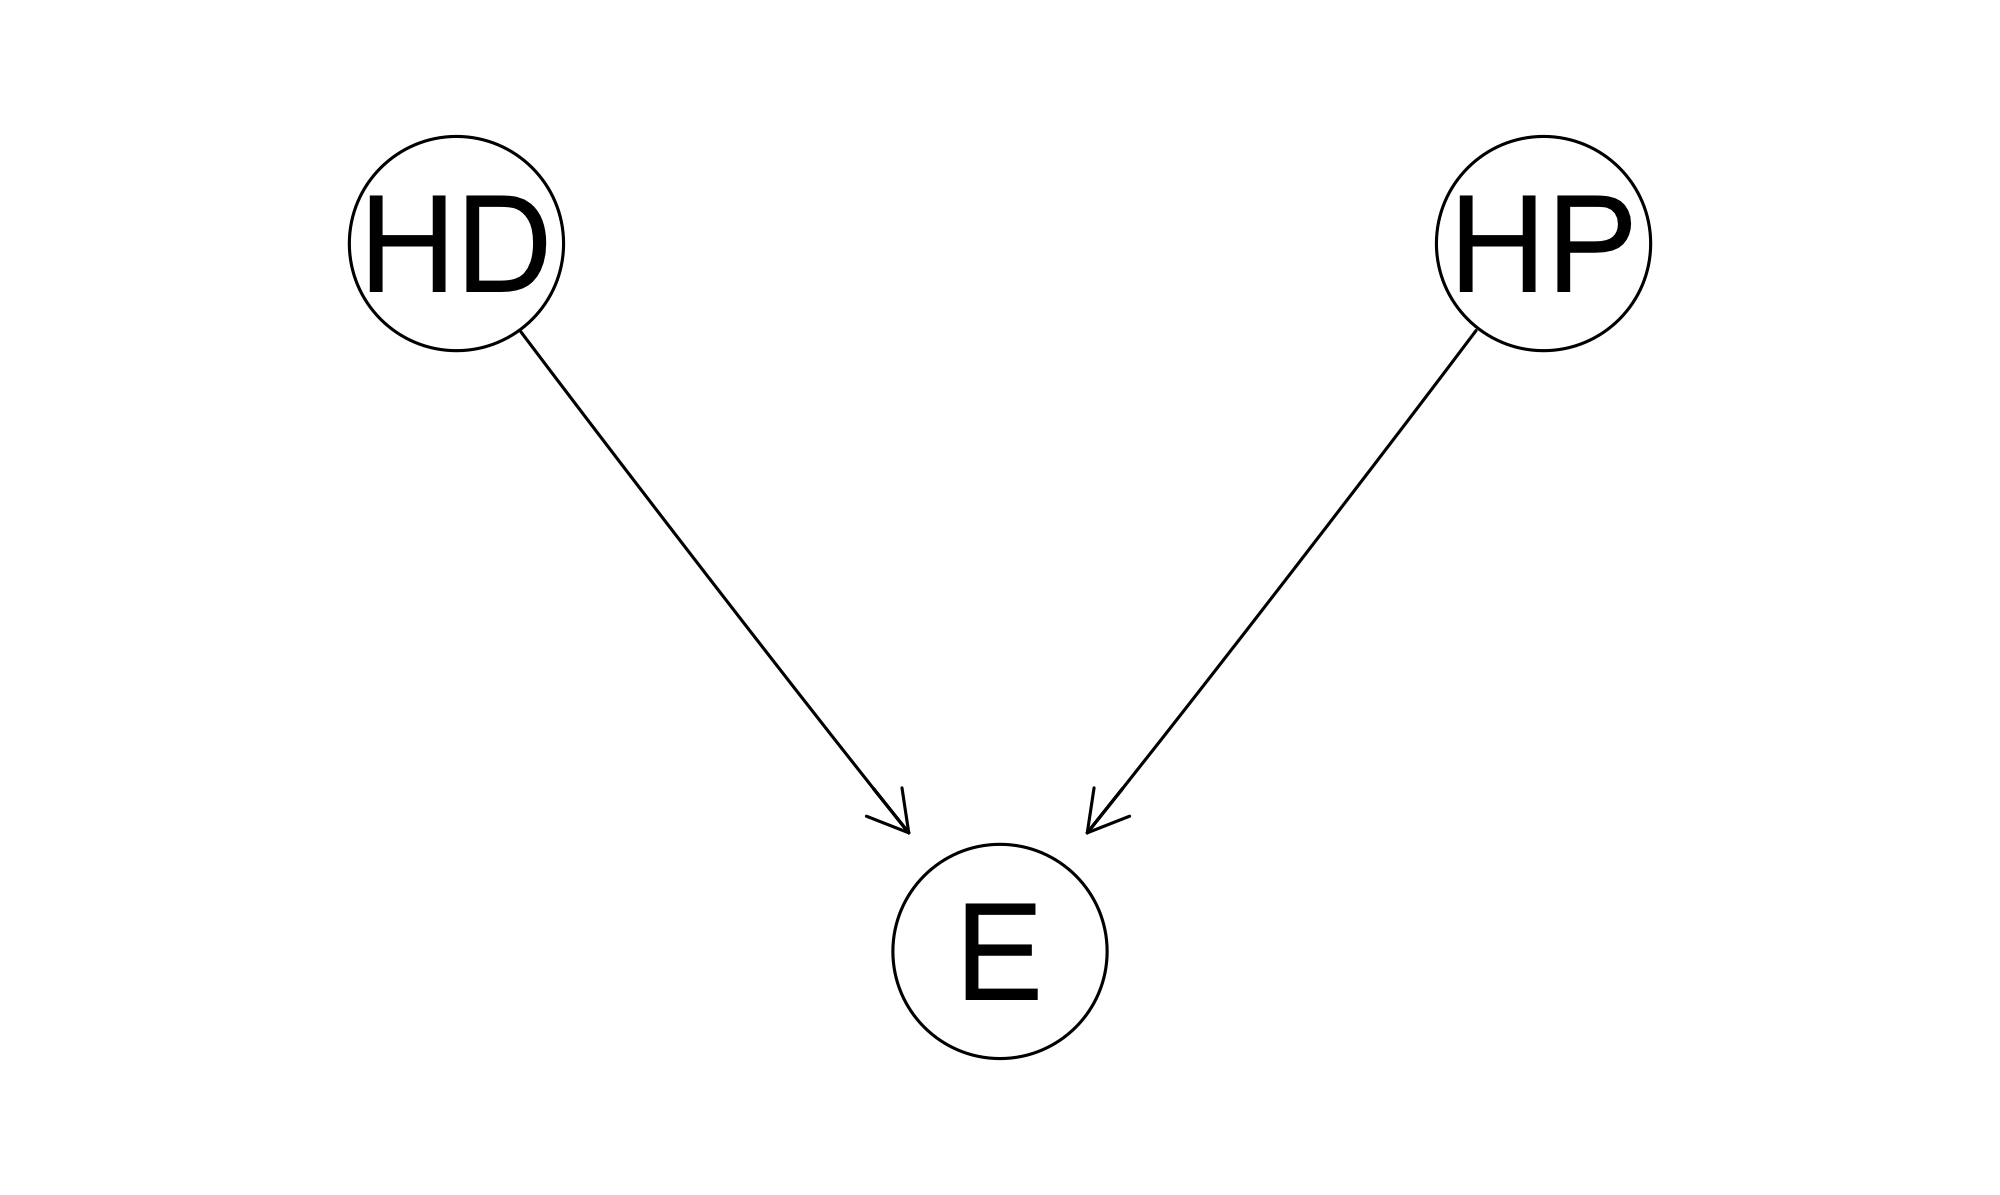
\includegraphics[scale = 0.08]{STMdag.png}}
        {\caption{\footnotesize Graphic model of Small Town Murder}\label{fig:bayes_test4}}
        \ffigbox{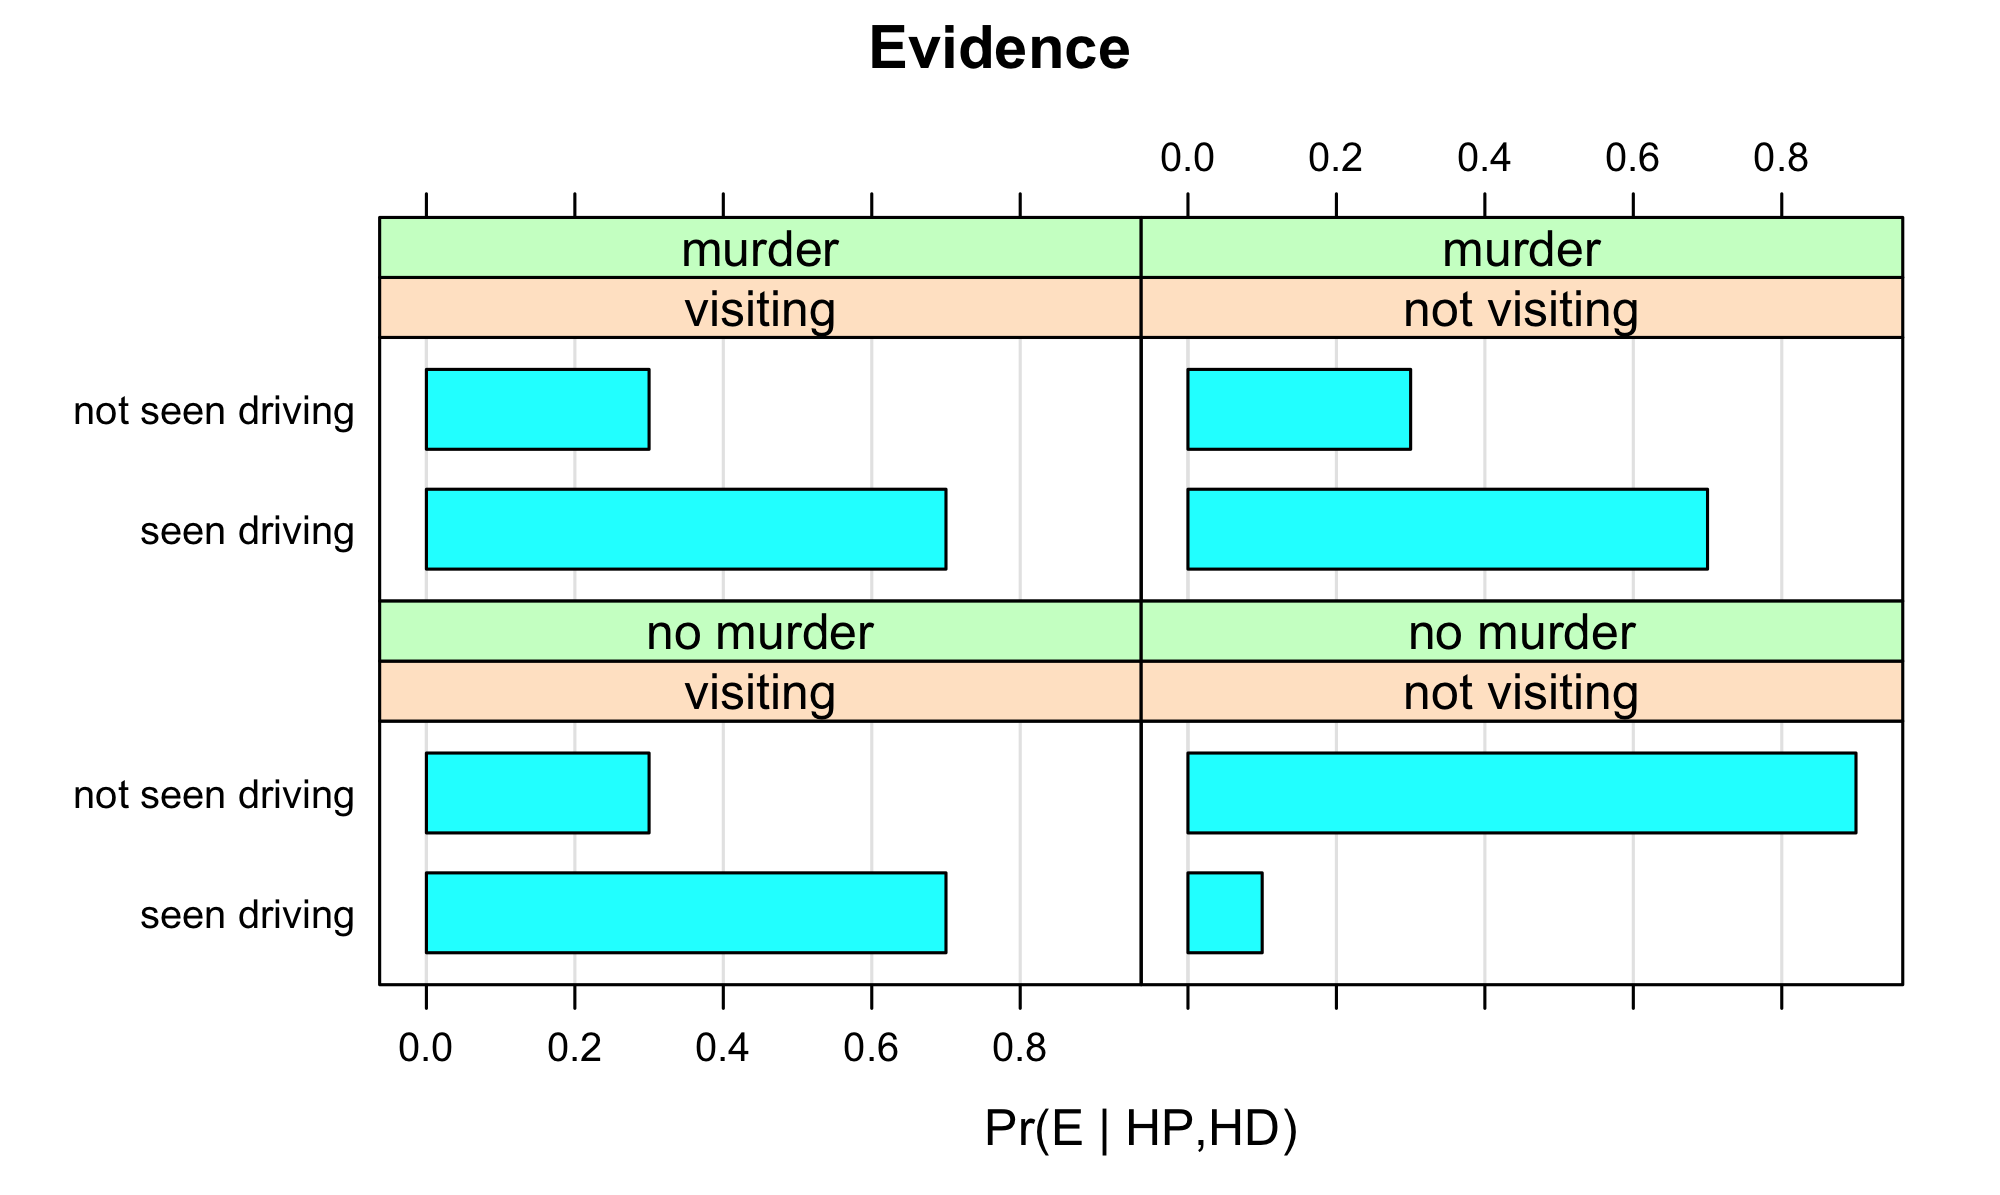
\includegraphics[scale = 0.08]{STMpt.png}}{
            \caption{\footnotesize Probability distribution of $E$}\label{fig:bayes_test6}}
    \end{floatrow}
\end{figure}

\%

\noindent
 Following the calculations in
\citep{dezoete2019ResolvingSocalledProbabilistic}, for exclusive and
exhaustive hypotheses, \(LR(E,H_d,\neg H_d)=1.75\), and similarly,
\(LR(E,H_p, \neg H_p)=1.75\), since \(P(E\vert H_d)=0.7\) and
\(P(E\vert \neg H_d)=0.4\). The likelihood ratio of the evidence, if it
is measured against exclusive and exhaustive hypotheses, is not equal to
one.\footnote{ \cite{dezoete2019ResolvingSocalledProbabilistic} offer a slightly different solution to the problem. They construct a Bayesian network with three hypotheses, also exhaustive and exclusive: in town to visit mother, in town to murder, out of town.}
Such considerations should also generalize to other paradoxes of
relevance.\\
\% \%For instance, in the twins problem, the LR is 1 if the hypotheses
are:
\texttt{the\ suspect\ committed\ the\ crime\textquotesingle{},\ and}the
suspect's twin brother committed the crime', but is not 1 f we consider
the fairly natural hypothesis that the defendant is innocent.
\%Similarly, \%In the food tray example, Bayesian network analysis shows
that the value of the evidence `prisoner withholds tray' for the
question who started the fight depends on a range of uncertain events
and other pieces of evidence (such as whether indeed a parcel he was
supposed to obtain was withheld; whether the prisoner inquired about
this; whether and how this inquiry was answered). Considered in this
context, the piece of evidence will not have a likelihood ratio of one
with respect to at least some choice of sensible hypotheses. \%

The general problem with the paradoxes of relevance is that in complex
situations there is no single likelihood ratio that corresponds to a
single piece of evidence. The problematic scenarios focus on a single
likelihood ratio based on non-exclusive or non-exhaustive hypotheses.
However, evidence can be relevant so long as it has a probabilistic
impact on a sub-hypothesis involved in the case, even without having a
recognizable probabilistic impact on the prosecutor's or defense's
ultimate hypotheses. When this happens, it is relevant, in agreement
with Rule 401 of the Federal Rules of Evidence. Bayesian networks help
to see how pieces of evidence can increase or decrease the probability
of different sub-hypotheses
\cite{dezoete2019ResolvingSocalledProbabilistic}.

\%recommend relying on a Bayesian network to investigate in an orderly
manner the way in which pieces of evidence and hypotheses
interact.\todo{no one said the interact in an orderly manner. ;) } \%in
an orderly manner.

\section{Conclusions}\label{conclusions}

Where are we, how did we get here, and where can we go from here? We
were looking for a probabilistically explicated condition \(\Psi\) such
that the trier of fact, at least ideally, should accept any relevant
claim (including \(G\)) just in case \(\Psi(A,E)\).

From the discussion that transpired it should be clear that we were
looking for a \(\Psi\) satisfying the following desiderata:

\begin{description}
\item[conjunction closure] If $\Psi(A,E)$ and $\Psi(B,E)$, then $\Psi(A\et B,E)$.
\item[naked statistics] The account should at least make it possible for convictions based on strong, but naked statistical evidence to be unjustified. 
\item[equal treatment] the condition should apply to any relevant claim whatsoever (and not just a selected claim, such as $G$).
\end{description}

Throughout the paper we focused on the first two conditions (formulated
in terms of the difficulty about conjunction (DAC), and the gatecrasher
paradox), going over various proposals of what \(\Psi\) should be like
and evaluating how they fare. The results can be summed up in the
following table:

\begin{center}
\footnotesize 
 \begin{tabular}{@{}p{3cm}p{2.5cm}p{4cm}p{3cm}@{}}
\toprule
\textbf{View} & \textbf{Convict iff} & \textbf{DAC} & \textbf{Gatecrasher} \\ \midrule
Threshold-based LP (TLP) & Probability of guilt given the evidence is above a certain threshold & fails & fails \\
Dawid's likelihood strategy & No condition given, focus on $\frac{\pr{H\vert E}}{\pr{H\vert \n E}}$ & - If evidence is fairly reliable, the posterior of $A\et B$ will be greater than the prior.

- The posterior of $A\et B$ can still be lower than the posterior of any of $A$ and $B$.

- Joint likelihood, contrary do Dawid's claim, can also be lower than any of the individual likelihoods. & fails  \\
Cheng's relative LP (RLP)
& Posterior of guilt higher than the posterior of any of the defending narrations & The solution assumes equal costs of errors and independence of $A$ and $B$ conditional on $E$. It also relies on there being multiple defending scenarios individualized in terms of  combinations of literals involving $A$ and $B$. & Assumes that the prior odds of guilt are 1, and that the statistics is not sensitive to guilt (which is dubious). If the latter fails, tells to convict as long as the prior of guilt $<0.991$. \\
Kaplow's decision-theoretic LP (DTLP) &
The likelihood of the evidence is higher than the odds of innocence multiplied by the cost of error ratio & fails & convict if cost ratio $<110.1111$
\end{tabular} 
 \end{center}

Thus, each account either simply fails to satisfy the desiderata, or
succeeds on rather unrealistic assumptions. Does this mean that a
probabilistic approach to legal evidence evaluation should be abandoned?
No. This only means that if we are to develop a general probabilistic
model of legal decision standards, we have to do better. One promising
direction is to go back to Cohen's pressure against
\textbf{Requirement 1} and push against it. A brief paper suggesting
this direction is (Di Bello, 2019b), where the idea is that the
probabilistic standard (be it a threshold or a comparative wrt.
defending narrations) should be applied to the whole claim put forward
by the plaintiff, and not to its elements. In such a context, DAC does
not arise, but \textbf{equal treatment} is violated. Perhaps, there are
independent reasons to abandon it, but the issue deserves further
discussion. Another strategy might be to go in the direction of
employing probabilistic methods to explicate the narration theory of
legal decision standards (Urbaniak, 2018), but a discussion of how this
approach relates to DAC and the gatecrasher paradox lies beyond the
scope of this paper.

\section{References}\label{references}

\hypertarget{refs}{}
\hypertarget{ref-arkesEtAl2012}{}
Arkes, H. R., Shoots-Reinhard, B. L., \& Mayes, R. S. (2012).
Disjunction between probability and verdict in juror decision making.
\emph{Journal of Behavioral Decision Making}, \emph{25}(3), 276--294.

\hypertarget{ref-Bernoulli1713Ars-conjectandi}{}
Bernoulli, J. (1713). \emph{Ars conjectandi}.

\hypertarget{ref-blome2015}{}
Blome-Tillmann, M. (2015). Sensitivity, causality, and statistical
evidence in courts of law. \emph{Thought: A Journal of Philosophy},
\emph{4}(2), 102--112.

\hypertarget{ref-buchak2014belief}{}
Buchak, L. (2014). Belief, credence, and norms. \emph{Philosophical
Studies}, \emph{169}(2), 285--311.

\hypertarget{ref-cheng2012reconceptualizing}{}
Cheng, E. (2012). Reconceptualizing the burden of proof. \emph{Yale LJ},
\emph{122}, 1254. HeinOnline.

\hypertarget{ref-cohen1988difficulty}{}
Cohen, L. J. (1988). The difficulty about conjunction in forensic proof.
\emph{The Statistician}, \emph{37}(4/5), 415. JSTOR. Retrieved from
\url{https://doi.org/10.2307/2348767}

\hypertarget{ref-dawid1987difficulty}{}
Dawid, A. P. (1987). The difficulty about conjunction. \emph{The
Statistician}, 91--97. JSTOR.

\hypertarget{ref-Dekay1996}{}
Dekay, M. L. (1996). The difference between Blackstone-like error ratios
and probabilistic standards of proof. \emph{Law and Social Inquiry},
\emph{21}, 95--132.

\hypertarget{ref-dhamiEtAl2015}{}
Dhami, M. K., Lundrigan, S., \& Mueller-Johnson, K. (2015). Instructions
on reasonable doubt: Defining the standard of proof and the jurors task.
\emph{Psychology, Public Policy, and Law, 21(2), 169178}, \emph{21}(2),
169--178.

\hypertarget{ref-diBello2019}{}
Di Bello, M. (2019a). Trial by statistics: Is a high probability of
guilt enough to convict? \emph{Mind}.

\hypertarget{ref-DiBello2019plausibility}{}
Di Bello, M. (2019b). Probability and plausibility in juridical proof.
\emph{International Journal of Evidence and Proof}.

\hypertarget{ref-diamond90}{}
Diamond, H. A. (1990). Reasonable doubt: To define, or not to define.
\emph{Columbia Law Review}, \emph{90}(6), 1716--1736.

\hypertarget{ref-ebert2018}{}
Ebert, P. A., Smith, M., \& Durbach, I. (2018). Lottery judgments: A
philosophical and experimental study. \emph{Philosophical Psychology},
\emph{31}(1), 110--138.

\hypertarget{ref-Enoch2012Statistical}{}
Enoch, D., Spectre, L., \& Fisher, T. (2012). Statistical evidence,
sensitivity, and the legal value of knowledge. \emph{Philosophy and
Public Affairs}, \emph{40}(3), 197--224.

\hypertarget{ref-friedman2015}{}
Friedman, O., \& Turri, J. (2015). Is probabilistic evidence a source of
knowledge? \emph{Cognitive Science}, \emph{39}(5), 1062--1080.

\hypertarget{ref-ho08}{}
Ho, H. L. (2008). \emph{Philosophy of evidence law}. Oxford University
Press.

\hypertarget{ref-Horowitz1996}{}
Horowitz, I. A., \& Kirkpatrick, L. C. (1996). A concept in search of a
definition: The effect of reasonable doubt instrcutions on certainty of
guilt standards and jury verdicts. \emph{Law and Human Behaviour},
\emph{20}(6), 655--670.

\hypertarget{ref-Kaplan1968decision}{}
Kaplan, J. (1968). Decision theory and the fact-finding process.
\emph{Stanford Law Review}, \emph{20}(6), 1065--1092.

\hypertarget{ref-kaplow2014likelihood}{}
Kaplow, L. (2014). Likelihood ratio tests and legal decision rules.
\emph{American Law and Economics Review}, \emph{16}(1), 1--39. Oxford
University Press.

\hypertarget{ref-kaye79}{}
Kaye, D. H. (1979a). The laws of probability and the law of the land.
\emph{The University of Chicago Law Review}, \emph{47}(1), 34--56.

\hypertarget{ref-Kaye79gate}{}
Kaye, D. H. (1979b). The paradox of the Gatecrasher and other stories.
\emph{The Arizona State Law Journal}, 101--110.

\hypertarget{ref-Laplace1814}{}
Laplace, P. (1814). \emph{Essai philosophique sur les probabilités}.

\hypertarget{ref-laudan2006truth}{}
Laudan, L. (2006). \emph{Truth, error, and criminal law: An essay in
legal epistemology}. Cambridge University Press.

\hypertarget{ref-Lempert1986}{}
Lempert, R. O. (1986). The new evidence scholarship: Analysing the
process of proof. \emph{Boston University Law Review}, \emph{66},
439--477.

\hypertarget{ref-moss2018}{}
Moss, S. (2018). \emph{Probabilistic knowledge}. Oxford University
Press.

\hypertarget{ref-newman1993}{}
Newman, J. O. (1993). Beyon ``reasonable doub''. \emph{New York
University Law Review}, \emph{68}(5), 979--1002.

\hypertarget{ref-niedermeierEtAl1999}{}
Niedermeier, K. E., Kerr, N. L., \& Messeé, L. A. (1999). Jurors' use of
naked statistical evidence: Exploring bases and implications of the
Wells effect. \emph{Journal of Personality and Social Psychology},
\emph{76}(4), 533--542.

\hypertarget{ref-nunn2015}{}
Nunn, A. G. (2015). The incompatibility of due process and naked
statistical evidence. \emph{Vanderbilt Law Review}, \emph{68}(5),
1407--1433.

\hypertarget{ref-pardo2018}{}
Pardo, M. S. (2018). Safety vs.~sensitivity: Possible worlds and the law
of evidence. \emph{Legal Theory}, \emph{24}(1), 50--75.

\hypertarget{ref-pritchard2015}{}
Pritchard, D. (2015). Risk. \emph{Metaphilosophy}, \emph{46}(3),
436--461.

\hypertarget{ref-pundik2017}{}
Pundik, A. (2017). Freedom and generalisation. \emph{Oxford Journal of
Legal Studies}, \emph{37}(1), 189--216.

\hypertarget{ref-Roth2010}{}
Roth, A. (2010). Safety in numbers? Deciding when DNA alone is enough to
convict. \emph{New York University Law Review}, \emph{85}(4),
1130--1185.

\hypertarget{ref-smith2017}{}
Smith, M. (2018). When does evidence suffice for conviction?
\emph{Mind}, \emph{127}(508), 1193--1218.

\hypertarget{ref-Stein05}{}
Stein, A. (2005). \emph{Foundations of evidence law}. Oxford University
Press.

\hypertarget{ref-sykes1999}{}
Sykes, D. L., \& Johnson, J. T. (1999). Probabilistic evidence versus
the representation of an event: The curious case of Mrs. Prob's dog.
\emph{Basic and Applied Social Psychology}, \emph{21}(3), 199--212.

\hypertarget{ref-Thomson86}{}
Thomson, J. J. (1986). Liability and individualized evidence. \emph{Law
and Contemporary Problems}, \emph{49}(3), 199--219.

\hypertarget{ref-urbaniak2018narration}{}
Urbaniak, R. (2018). Narration in judiciary fact-finding: A
probabilistic explication. \emph{Artificial Intelligence and Law},
1--32.

\hypertarget{ref-walen2015}{}
Walen, A. (2015). Proof beyond a reasonable doubt: A balanced
retributive account. \emph{Louisiana Law Review}, \emph{76}(2),
355--446.

\hypertarget{ref-Wasserman91}{}
Wasserman, D. T. (1991). The morality of statistical proof and the risk
of mistaken liability. \emph{Cardozo Law Review}, \emph{13}, 935--976.

\end{document}
